% ------------------------------------------------------------------------
% MS Thesis of Juan de la Cruz
% Date Defended: May 31, 2000
% ------------------------------------------------------------------------
\documentclass[letterpaper,12pt]{report}
\usepackage[centertags]{amsmath}
\usepackage{amsfonts}
\usepackage{amssymb}
\usepackage{amsthm}
\usepackage{newlfont}
\usepackage{epsfig}
\usepackage{UPCSTHESIS} %This loads the UP Computer Science Thesis Package
\usepackage{UPCSINC1}
\usepackage[active]{LTX}
\usepackage{subfigure}
\usepackage{listings}
\usepackage{array}
\usepackage{graphicx}
\usepackage[table]{xcolor}
\usepackage{url}
\usepackage{fancyhdr}
\usepackage{lscape}
\usepackage{float}
\usepackage{booktabs}
\usepackage{caption}
\usepackage{amsmath,amssymb}
\usepackage{siunitx}
\usepackage[hidelinks]{hyperref}
\usepackage{enumitem}
\usepackage{titlesec}
\usepackage[backend=biber,style=numeric,sorting=none]{biblatex}
\usepackage[table]{xcolor}
\usepackage{algorithm}
\usepackage{algpseudocode}
\addbibresource{references.bib} 

\fancyhf{} % clear all header and footer fields
\fancyfoot[C]{\thepage}
\renewcommand{\headrulewidth}{0pt}
\renewcommand{\footrulewidth}{0pt}

% Redefining plain style which is automatically applied to chapters (including Bibliography)

\fancypagestyle{plain}{%
\fancyhf{} % clear all header and footer fields
\fancyfoot[C]{\thepage}
\renewcommand{\headrulewidth}{0pt}
\renewcommand{\footrulewidth}{0pt}
}
\pagestyle{fancy} 

%% Define a new 'leo' style for the package that will use a smaller font.
\makeatletter
\def\url@leostyle{%
  \@ifundefined{selectfont}{\def\UrlFont{\sf}}{\def\UrlFont{\small\ttfamily}}}
\makeatother
%% Now actually use the newly defined style.
\urlstyle{leo}


\hfuzz2pt
\newlength{\defbaselineskip}
\setlength{\defbaselineskip}{\baselineskip}
\newcommand{\setlinespacing}[1]%
           {\setlength{\baselineskip}{#1 \defbaselineskip}}
\newcommand{\doublespacing}{\setlength{\baselineskip}%
                           {2.0 \defbaselineskip}}
\newcommand{\singlespacing}{\setlength{\baselineskip}{\defbaselineskip}}
% MATH -------------------------------------------------------------------
\newcommand{\A}{{\cal A}}
\newcommand{\h}{{\cal H}}
\newcommand{\s}{{\cal S}}
\newcommand{\W}{{\cal W}}
\newcommand{\BH}{\mathbf B(\cal H)}
\newcommand{\KH}{\cal  K(\cal H)}
\newcommand{\Real}{\mathbb R}
\newcommand{\Complex}{\mathbb C}
\newcommand{\Field}{\mathbb F}
\newcommand{\RPlus}{[0,\infty)}
\newcommand{\norm}[1]{\left\Vert#1\right\Vert}
\newcommand{\essnorm}[1]{\norm{#1}_{\text{\rm\normalshape ess}}}
\newcommand{\abs}[1]{\left\vert#1\right\vert}
\newcommand{\set}[1]{\left\{#1\right\}}
\newcommand{\seq}[1]{\left<#1\right>}
\newcommand{\eps}{\varepsilon}
\newcommand{\To}{\longrightarrow}
\newcommand{\RE}{\operatorname{Re}}
\newcommand{\IM}{\operatorname{Im}}
\newcommand{\Poly}{{\cal{P}}(E)}
\newcommand{\EssD}{{\cal{D}}}
% THEOREMS ---------------------------------------------------------------
\theoremstyle{plain}
\newtheorem{thm}{Theorem}[section]
\newtheorem{cor}[thm]{Corollary}
\newtheorem{lem}[thm]{Lemma}
\newtheorem{prop}[thm]{Proposition}
\theoremstyle{definition}
\newtheorem{defn}{Definition}[section]
\theoremstyle{remark}
\newtheorem{rem}{Remark}[section]
\numberwithin{equation}{section}
\renewcommand{\theequation}{\thesection.\arabic{equation}}
\setlength{\tclineskip}{1.05\baselineskip}

\begin{document}

%\nobib  			%toggles bibliography control
%\draft				%toggles draft printing
%\nofront			%toggles nofront printing

\permissionfalse

%\nolistoftables	%toggles table control
%\nolistoffigures	toggles figures

% ------------------------------------------------------------------------

\title{TradeLENS: CNN-Based Trading Strategy with Integrated Technical and Macroeconomic Representations}

\bs
\author{Vall James P. Luceres}
\degreeinitial{B.S.C.S.}
\major{Computer Science}
\adviser{ASST. PROF. Ryan Rey M. Daga}
\firstreader{Mr. Allan Fritzgerald N. Amistoso}
\secondreader{Mr. Samson Jr. D. Rollo}
\dean{Dr. Patricia B. Arinto}
\submityear{May 2026}
\studentid{2021-07318}

% ------------------------------------------------------------------------
{
%\WinEdt{?0000} % Don't bother with over/under-full boxes
%\beforepreface
%\WinEdt{?1111} % Process All Errors from Here on
\forgeterr{?0000} % Don't bother with over/under-full boxes
\beforepreface
\forgeterr{?1111} % Process All Errors from Here on
}

{
\typeout{Acknowledgements}
\prefacesection{Acknowledgements}

This research was completed through the guidance and support of many people who became part of this journey.

I express my deepest gratitude to my research adviser, Ryan Rey M. Daga, for his guidance, patience, and support throughout this study. His comments and suggestions helped me understand the direction of the work more clearly. His advice also helped me improve both the technical and written parts of this research, especially during the stages where the study needed refinement.

I would also like to thank the panel members for their valuable comments and recommendations. Their feedback helped me see the study from a better perspective and guided me in strengthening the important parts of this research.

To my coursemates, Julius and Matthew, thank you for being part of this journey. The shared discussions, struggles, and small moments of encouragement made the process easier to carry. Having people who understood the pressure of thesis work helped me continue during the moments when progress felt difficult. To my friends, Gabriel and Josh, for making me laugh and the encouragement throughout this journey. Your presence helped make the difficult parts lighter. 

To Merielle, thank you for always being there for me when I needed a source of comfort and patience. Your support helped me stay grounded during the most stressful parts of this research. I am grateful for the understanding, care, and quiet strength you gave me when I needed it most.

To my family, thank you for your love, patience, and support. Thank you for understanding the time and effort that this work required. Your encouragement gave me strength throughout my studies, and this thesis is also a reflection of the support you have given me.

I would also like to acknowledge the researchers, developers, and open-source communities whose works helped make this study possible. Their contributions served as important references in building and evaluating the system developed in this research.

Finally, I am thankful to everyone who supported me in any way throughout this thesis. Every piece of advice, encouragement, and help became part of the reason this work was completed.

}
% ------------------------------------------------------------------------
{
\typeout{Abstract}
\prefacesection{Abstract}

Market behavior is shaped not only by price movements but also by macroeconomic forces that influence price stability. Current quantitative trading systems built on convolutional neural networks (CNNs) typically represent market dynamics using technical indicator-derived images. However, these models often ignore macroeconomic indicators that significantly influence financial returns. This study introduces TradeLENS (Trade Learning with Economic and Numeric Signals), a CNN-based trading framework that integrates 15 technical indicators and 5 selected macroeconomic indicators into a unified grayscale image representation to determine the appropriate trading action (Buy, Hold, or Sell). For each trading day, a 20$\times$20 pixel image was constructed from a 20-period lookback window of technical and macroeconomic indicators, and labeled as BUY, SELL, or HOLD using a fixed-window turning-point labeling method. Although the proposed model yielded lower classification accuracy (64.76\%) than the technical-only model (69.24\%), it demonstrated superior trading outcomes. Starting from an initial equity of PHP 10,000, it achieved a final equity of PHP 21,715.91 and a mean annual return of 16.55\%, compared to PHP 17,384.65 and 11.32\% for the baseline. SHAP analysis further supported these empirical results by showing that selected macroeconomic indicators received higher feature importance in profitable CNN--MIC predictions. These findings suggest that incorporating macroeconomic indicators, despite not improving classification accuracy, enhances the profitability of the generated trading signals and underscores the practical value of macroeconomic context in CNN-based trading systems.


	%\textit{Keywords}: Deep-learning; image classification; trading indicators; macroeconomic-informed representations; quantitative trading strategies

}
\tableofcontentspage
% ------------------------------------------------------------------------
%\setcounter{page}{1}
%\tableofcontents
% ------------------------------------------------------------------------

% ------------------------------------------------------------------------
\afterpreface
\def\baselinestretch{1}
\setlinespacing{1.66}
% ------------------------------------------------------------------------
{
%\typeout{Introduction}
%\include{introd}
}
% ------------------------------------------------------------------------
\setlinespacing{1.66}
% ------------------------------------------------------------------------

%!TEX root = thesis.tex
\chapter{Introduction}\label{chap:intro} 

\section{Background of the Study}

Market behavior is shaped not only by price movements but also by the broader economic context that affects risk, liquidity, and investor behavior. Over the past decade, computer vision-based models have become a popular tool that convert price data into images and train Convolutional Neural Networks (CNN) to generate \textit{Buy/Hold/Sell} decisions \cite{cohen2020trading,sezer2018algorithmic,gudelek2017deep}. These are effective in capturing local patterns of time and price. However they usually treat the macroeconomic context separately, which has a clear contribution to changing market prices \cite{wang2019aggregating,ma2022macroeconomic,chauhan2025exploring}.

This study aims to improve existing image-based representations by merging technical and macroeconomic indicators into a unified image representation so that it can be processed by our proposed CNN model. 
The model takes into account strict time adaptation, uniform normalization, and careful encoding to preserve the relationship between local patterns and market context \cite{sezer2018algorithmic,maratkhan2021deep}. 
The framework is applied to selected Philippine blue-chip, penny stocks, and cryptocurrency, where the impact of incorporating macroeconomic indicators on prediction accuracy and performance metrics is measured.


\section{Basic Definitions and Notations}\label{sec:BasicDefns}
\subsubsection*{Quantitative Trading using Image Classification}
Quantitative trading is a system that automates trades that are conducted using models and technical indicators as tools \cite{ta2018prediction}. It can be represented in images that are in a grid of indicators and time windows, to allow spatial filters to uncover patterns that match price movement \cite{cohen2020trading,sezer2018algorithmic}. Representations such as candlesticks, bar charts, and technical indicators as images can improve trend classification and transaction signals \cite{gudelek2017deep,chen2020encoding,liu2023automated}. Transforming financial time series into visual representations enables machine learning algorithms to efficiently recover complex trading signals \cite{cohen2020trading}, with candlestick image data consistently outperforming traditional numeric approaches \cite{liu2023automated}. 


\subsubsection*{CNN-based Technical Indicator Clustering (CNN--TIC)}

Convolutional neural networks are structured to learn spatial patterns from grid-formatted data, which makes them well suited for technical indicators arranged as two-dimensional images \cite{al2017understanding,lecun1995learning}. Early image-based trading studies demonstrated that converting technical indicators into fixed-size grayscale images allows a CNN to detect local price and momentum patterns more effectively than traditional numeric inputs \cite{sezer2018algorithmic}. This established image representation as a practical way to capture short-term market patterns.

Later work organized technical indicators into clustered channels, forming what is now known as the CNN--TIC model \cite{maratkhan2021deep}. In that model, fifteen technical indicators were used to represent market behavior: Relative Strength Index (RSI), Williams~\%R, Simple Moving Average (SMA), Exponential Moving Average (EMA), Weighted Moving Average (WMA), Hull Moving Average (HMA), Triple Exponential Moving Average (TEMA), Commodity Channel Index (CCI), Chande Momentum Oscillator (CMO), Moving Average Convergence Divergence (MACD), Percentage Price Oscillator (PPO), Rate of Change (ROC), Chaikin Money Flow Indicator (CMFI), Directional Movement Indicator (DMI), and Parabolic Stop and Reverse Indicator (PSI) \cite{maratkhan2021deep}.

These indicators describe different aspects of price behavior. RSI, Williams~\%R, CCI, CMO, MACD, PPO, ROC, DMI, and PSI measure momentum, trend direction, or possible reversal behavior. SMA, EMA, WMA, HMA, and TEMA describe smoothed price trends using different weighting schemes. CMFI adds volume information by estimating whether buying or selling pressure is supported by trading volume. In general, these indicators are derived from OHLCV data through moving averages, price differences, high--low ranges, momentum ratios, or volume-weighted price relationships over a defined lookback window \cite{wilder1978new,murphy1999technical,achelis2001technical}.

In CNN--TIC, these indicators were grouped into separate channels based on similarity in behavior, allowing the model to process related technical indicators within the same representation \cite{maratkhan2021deep}. This makes CNN--TIC an appropriate baseline for this study, since it uses image-based technical indicator representations for Buy, Hold, and Sell classification.

\subsubsection*{Multimodal Approach}
In deep learning, multimodal processing refers to the integration of data from different types to increase the learning efficiency and performance of algorithms on a specific task \cite{dimitri2022short}. This approach is advantageous because each modality responds to different characteristics and provides complementary information that is not fully captured by a single form of data. For example, visual data can support and validate the content of spoken language, while textual data can explain the content of visual cues. In the context of the financial market, the technical picture from OHLCV (Open, High, Low, Close, Volume) data depicts local patterns over time and price, while textual policy statements, earnings reports, and sentiment measures on social media provide a more slowly evolving context of market environment and risk \cite{farimani2024adaptive,karadacs2025multimodal}.

These representations provide a broader range of signals that can help to understand the change and risk of the market environment \cite{zhang2020multimodal}. Fusion can be viewed as the combination of different modalities into a single meaning space, so that the learned patterns are richer, more robust to noise, and more appropriate to different market conditions. Additionally, it can also be presented in a form that is well-suited for learning that can improve classification and prediction compared to relying on a single approach \cite{gallo2018image}. 

\subsubsection*{Macroeconomic Representation}
Macroeconomic representations are economic signals such as interest rates, inflation, exchange rates, market volatility, and foreign investment, that reflect the state of the market environment at a given time \cite{artantacs2020selected}. These indicators represent the broader economic conditions that influence market behavior, investor sentiments, liquidity, and overall financial returns \cite{Naik02012024,mazumder2025impact}. This is relevant because literature shows that macroeconomic attention and policy uncertainty are significantly linked to expected short- and long-term earnings and sector dynamics \cite{ma2022macroeconomic}. In this view, the macro series becomes the “context” that moves slowly and shapes the course of the market and liquidity, while technical indicators from OHLCV represent the faster, more localized patterns. It is important to describe these signals in a consistent form and scale that can be related to the technical representation \cite{wang2019aggregating}.

For this study, five macroeconomic indicators were selected: Reverse Repurchase Rate (RRP), gold price, crude oil price, purchasing power of the peso (PPP), and inflation rate. The RRP represents the monetary policy stance of the Bangko Sentral ng Pilipinas and reflects the rate used in its reverse repurchase operations \cite{bsp2025rrp}. Gold price was included as an indicator of uncertainty and store-of-value demand, while crude oil price was included because energy prices affect production costs, inflation pressure, and broader economic activity \cite{worldbank2025commoditymarkets,mazumder2025impact}. PPP refers to the purchasing power of the peso which represents the real value of the peso relative to a reference period using the Consumer Price Index \cite{psa2020ppp}. Inflation rate was included because it measures changes in consumer prices and reflects the price stability of the economy \cite{psa2025cpi}.

Together, these indicators provide a compact representation of the macroeconomic setting surrounding each trading day. RRP captures monetary policy conditions, gold captures uncertainty-related conditions, crude oil captures energy-related cost pressure, PPP captures the real value of the peso, and inflation captures general price movement. These variables are aligned with the trading calendar and normalized into a common grayscale range so that CNN--MIC can process macroeconomic context together with technical patterns in a single image representation.

\section{Problem Statement}\label{sec:ResearchQ}
\begin{figure}[H]
	\centering
	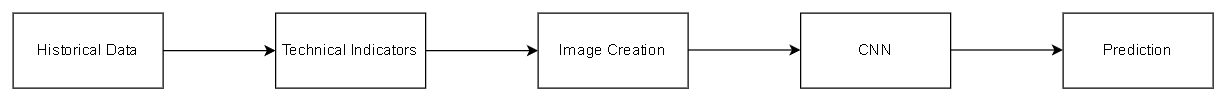
\includegraphics[width=0.8\textwidth]{../figures/CNN-TIC.png}
	\caption{Computer-vision trading using technical indicators}
	\label{Figure 1: Computer-vision trading using technical indicators}
\end{figure}


Figure~\ref{Figure 1: Computer-vision trading using technical indicators}  illustrates a typical single-mode workflow where historical price data are transformed into technical indicators, arranged as two-dimensional images, and passed through a CNN to generate trading signals \cite{sezer2018algorithmic,gudelek2017deep}. This setup is effective in capturing local price-time patterns because convolutional filters can highlight short-term structures on the image \cite{cohen2020trading}. However, the representation is restricted to indicators derived from OHLCV and does not explicitly incorporate macroeconomic information that shapes market risk, liquidity, and trend formation.

As a result, current CNN-based image models provide an incomplete view of the market environment. Broader conditions such as changes in interest rates, inflation, or policy-related uncertainty are not encoded in the same space as the technical picture, even if they have a documented effect on asset returns \cite{wang2019aggregating,ma2022macroeconomic,chauhan2025exploring}. In simple terms, existing CNN trading systems operate only on technical indicator images, and there is no unified image representation where technical signals and macroeconomic indicators are jointly organized, aligned, and scaled. This gap is the main problem that the study aims to address.

\section{Aim of the Work}
\subsection{General Objective}

\noindent Develop and evaluate an enhanced CNN-based trading model that integrates both technical and macroeconomic indicators to assess their effect on financial market trend prediction and trading performance.

\subsection{Specific Objectives}
\begin{enumerate}
	\item To enhance the CNN--TIC framework by expanding its technical indicator image matrix to include macroeconomic variables, forming a unified visual representation.
	\item To compare model performance using metrics such as accuracy, F1-score, and annualized return, to determine whether the inclusion of macroeconomic indicators leads to significant improvements.
	\item To evaluate performance on different stock categories in the PSE market and cryptocurrency.
	\item To evaluate feature importance and model behavior, interpret how macroeconomic information contributes to CNN decision-making in the context of financial trend prediction.
\end{enumerate}


\subsection{Scope and Limitation}
Previous studies on quantitative trading involve only CNNs that are solely trained on technical indicators as image representations. In such settings, the absence of macroeconomic information may limit the robustness and accuracy of the resulting models. Thus, this study aims to develop and evaluate a CNN-based trading framework that integrates both technical and macroeconomic indicators into a single image representation for market trend prediction.

The model will be tested on different stocks of the Philippine Stock Exchange (PSE) market, and will further include cryptocurrency data. The dataset will include historical daily price data, trading volumes, and selected macroeconomic indicators such as reverse repurchase (RRP), purchasing power of peso, inflation rate, gold, and crude oil. Meanwhile, the technical indicators that will be used are  Relative Strength Index (RSI), Williams~\%R, Simple Moving Average (SMA), Exponential Moving Average (EMA), Weighted Moving Average (WMA), Hull Moving Average (HMA), Triple Exponential Moving Average (TEMA), Commodity Channel Index (CCI), Chande Momentum Oscillator (CMO), Moving Average Convergence Divergence (MACD), Percentage Price Oscillator (PPO), Rate of Change (ROC), Chaikin Money Flow Indicator (CMFI), Directional Movement Indicator (DMI), and Parabolic Stop and Reverse Indicator (PSI).

Although quantitative trading is focused on financial market prediction, this study will only focus on stock data from the Philippine market, which may limit its applicability to other stock markets with different economic conditions. Additionally, trading simulations used a fixed commision of 50 pesos per trade and ignores market slippage. Nonetheless, this study aims to develop a structured framework to identify how macroeconomic integrated visual representations can enhance CNN-based trading performance across various market conditions.

\subsection{Significance of the Study}
With the growing interest in applying computer vision for market trend prediction, the need to show how we can incorporate both technical and macroeconomic indicators into a single image representation becomes even more important. Unlike traditional CNN models that solely rely on technical indicators, the proposed CNN framework aims to improve predictive accuracy and financial returns across different market conditions that are driven by macroeconomic factors.

The research will contribute to developing more adaptive quantitative trading systems that supports data-driven decision-making for traders and financial institutions. Academically, it extends computer vision applications in finance and provides a reproducible foundation for future studies on financial forecasting.




 %iintroduction


\chapter{Review of Related Literature}\label{sec:RRL}
The evolution of financial market prediction using computer vision is slowly becoming a popular tool used in trading. Previous studies surrounding market prediction can be categorized into three categories. To start, we have numerical models that are solely trained on technical indicators. Another approach is by using computer vision, which analyzes chart-based or image representations of price series. Lastly, multimodal fusion models that cover signals such as prices, technical indicators, and macroeconomic variables to improve prediction performance.

Chakole et al.\ \cite{chakole2021convolutional} introduced a Deep Trend Following (DTF) strategy that uses CNN prediction with market trend signals. The approach focuses on generating trading decisions based on the current and predicted future price of stocks. Results showed that their model provided a much better performance than traditional buy-and-hold models. Similar to this method, Saud et al.\ \cite{saud2024technical} used technical indicators such as MACD, DMI, and KST with LSTM models and GRU networks that can be used to develop intelligent strategies to predict stock trading signals. Their study showed that the MACD-based approach was the safest and most effective approach among other models. These results reinforce the role of technical indicators as a strong foundation for quantitative trading models.

Computer vision offers another effective approach for financial market prediction. 
Unlike traditional numerical models, image-based methods convert temporal market information into structured visual representations such as candlestick images, bar-chart images, Gramian Angular Fields, recurrence plots, or technical indicator grids. 
This transformation is useful because it allows convolutional filters to process local spatial patterns that correspond to temporal relationships in the original series. 
Wang and Oates showed that time-series data can be encoded as images using Gramian Angular Fields and Markov Transition Fields, allowing CNN-based models to learn discriminative patterns from visualized temporal structures \cite{wang2015encoding}. 
Hatami et al. also showed that recurrence plots can transform time-series data into two-dimensional texture-like images, making time-series classification suitable for CNN-based image recognition \cite{hatami2018classification}. 

In financial applications, this idea is consistent with the way traders visually interpret chart patterns before making decisions. 
Cohen et al. \cite{cohen2020trading} treated trading as an image classification task by transforming financial time-series data into visual forms. 
Sezer and Ozbayoglu \cite{sezer2018algorithmic} further demonstrated that financial indicators can be converted into two-dimensional image-like representations for CNN-based algorithmic trading. 
Chen and Tsai \cite{chen2020encoding} used Gramian Angular Fields to encode candlestick data as images and showed that CNNs can recognize candlestick patterns from these transformed representations. 
Liu and Kang \cite{liu2023automated} further supported this direction by showing that candlestick-based representations can be used in cryptocurrency trading models and can outperform purely numeric representations in their experimental setting.
These studies support the use of image-based encoding because temporal signals become organized into spatial patterns that CNN filters can analyze.

The effectiveness of translating financial data into images is strongly demonstrated by a progression of studies from Sezer \cite{sezer2018algorithmic}. Building on earlier work that converted indicators into images (CNN-TA) and used bar-chart images (CNN-BI), Maratkhan et al.\ \cite{maratkhan2021deep} presented a highly optimized pipeline. Their architectures (CNN--TIC, EO--CNN--TIC, ResNet--TA) clustered technical indicators into multi-channel images and used an optimized trading layer to achieve remarkable results: ``Buy/Sell'' recall scores up to $0.94/0.96$ and average annual returns on DOW-30 up to $36.70\%$, substantially outperforming buy-and-hold and their own reproduced baselines. In addition, Wu \cite{wu2021empowering} specifically highlighted that computer vision techniques can address technical analysis objectives like predicting bullish/bearish trends. Then in 2019, Chen et al.\ \cite{chen2020encoding} developed approaches to automatically recognize candlestick patterns with over $80\%$ accuracy using convolutional neural networks, providing strong evidence for the effectiveness of visual representation in trading.

Studies on financial market forecasting also utilized multimodal fusion frameworks to enhance prediction accuracy by integrating different data sources. Wang et al.\ \cite{wang2019aggregating} pioneered a model-independent framework that successfully incorporated trading volume, intraday return series, and investors’ social media emotions to forecast market trends. This study demonstrates that combining multiple information sources significantly outperforms single-method approaches in financial market prediction. Ma et al.\ \cite{ma2022macroeconomic} proved that macroeconomic attention indices (MAI) can predict stock market returns by components that are extracted using partial least squares (PLS) and the LASSO method. Chauhan et al.\ \cite{chauhan2025exploring} had a similar study that used an ARDL model to reveal how macroeconomic indicators like Foreign Institutional Investment (FII) and Economic Policy Uncertainty (EPU) influence stock returns over both short- and long-term market behavior.

Finally, researchers have fused textual and numerical data. Mo et al.\ \cite{mo2024mof} proposed a system that addresses key limitations in traditional stock prediction models by integrating policy and stock review texts with price data. The mechanism uses MacBERT to generate feature vectors and combine them with stock price data to be processed on a neural network. Similarly, Rahul Modak et al.\ \cite{Modak2023MarketSA} developed a multimodal transformer architecture that integrates earnings call transcripts, social media content, and technical market indicators, achieving $87.2\%$ sentiment classification accuracy compared to $78.4\%$ for unimodal baselines.

 %RRL
\chapter{Methodology}

\begin{figure}[H]
	\centering
	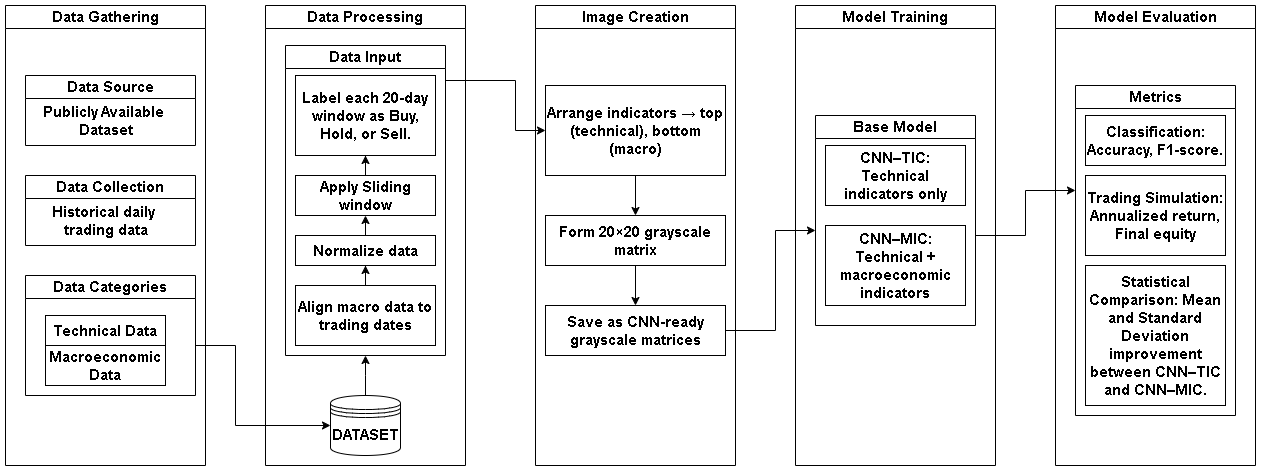
\includegraphics[width=1\textwidth]{../figures/Proposed Framework.png}
	\caption{Proposed Approach}
	\label{Figure 3: Proposed Framework}
\end{figure}


Figure~\ref{Figure 3: Proposed Framework} outlines the five stages of our methodology: (1)Data Gathering, (2)Data Processing, (3)Image Creation, (4)Model Training, and (5)Model Evaluation. The flow is centered on building an image representation of the combined technical and macroeconomic indicators using 20 lookback windows $L \in \{6,\ldots,25\}$ for each trading day.


\subsection{Data Gathering}
\label{subsec:data-gathering}

Open, High, Low, Close, and Volume (OHLCV) data from 2012 to August 2025 were collected for the selected PSE stocks and cryptocurrency assets. These values served as the basis for computing the technical indicators used in the image creation stage. In addition, five macroeconomic series were collected to represent the broader market environment: Reverse Repurchase (RRP), purchasing power of the peso (PPP), inflation rate, gold, and crude oil.

\subsection{Data Processing} \label{subsec:data-processing}
This stage ensures proper \emph{time alignment}, \emph{normalization}, and \emph{labeling} before creating images. We process two groups of variables in parallel, the technical indicators and the macroeconomic indicators, and merge them in \emph{Image Creation}.

\subsubsection*{(A) Processing of the technical indicators}

Following the technical indicator set used in CNN--TIC, the following 15 technical indicators are computed using the \texttt{ta} Python library~\cite{ta-bukosabino}: RSI, Williams~\%R, SMA, EMA, WMA, HMA, TEMA, CCI, CMO, MACD, PPO, ROC, CMFI, DMI, and PSI. These indicators are derived from OHLCV values and represent four main types of market information. First, trend indicators such as SMA, EMA, WMA, HMA, and TEMA summarize the direction of price movement by smoothing closing prices across a lookback window. Second, momentum indicators such as RSI, Williams~\%R, CMO, MACD, PPO, and ROC measure the speed, strength, or direction of price changes. Third, range-based indicators such as CCI, DMI, and PSI use high, low, and close values to describe trend strength, reversal behavior, or deviation from a typical price level. Finally, CMFI incorporates volume by measuring whether buying or selling pressure is supported by traded volume. These definitions follow common technical analysis formulations, while the actual computation in this study follows the implementation provided by the \texttt{ta} library~\cite{wilder1978new,murphy1999technical,achelis2001technical,ta-bukosabino}.

For each indicator $i$ and each lookback length $L \in \{6,7,\ldots,25\}$, we obtain the daily value
\[
x_{i,L,t} \;\; \text{for trading day } t.
\]
Here, $x_{i,L,t}$ denotes the value of technical indicator $i$ computed using lookback length $L$ for trading day $t$. Each lookback length produces one column in the technical image representation. Thus, one indicator generates 20 values per trading day, corresponding to window lengths from 6 to 25 days. Since there are 15 technical indicators, the technical-only representation contains $15 \times 20$ values before normalization and quantization.

For single-window indicators, $L$ sets the main computation window. For multi-parameter indicators such as MACD and PPO, $L$ controls the primary window according to the standard parameterization used by the library unless otherwise specified in the implementation. This step produces a structured technical feature matrix where rows correspond to indicators and columns correspond to lookback windows.
\subsubsection*{(B) Processing of the macroeconomic indicators}
Five macroeconomic indicators are aligned to the trading calendar with forward‑fill for non‑trading days: \textbf{RRP}, \textbf{PPP}, \textbf{inflation rate}, \textbf{gold}, and \textbf{crude oil}. To mirror the technical indicator format, we compute simple moving averages at the same set of lookbacks:
\[
\mathrm{SMA}_{m,L,t} = \frac{1}{L} \sum_{k=0}^{L-1} s_{m,t-k}, \qquad L \in \{6,\ldots,25\},
\]
where $s_{m,t}$ is the level of the macro series $m$ on day $t$.
\paragraph{Normalization and 8‑bit quantization.}
Each feature–lookback pair is first normalized with training‑only statistics, then quantized to unsigned 8‑bit:
\[
\tilde{v}_{r,L,t} = \operatorname{clip}\!\left(\frac{v_{r,L,t} - a_{r,L}}{b_{r,L} - a_{r,L} + \epsilon}, 0, 1\right),
\]
\[
\widehat{v}_{r,L,t} = \operatorname{round}\!\big(255 \cdot \tilde{v}_{r,L,t}\big) \in \{0,\ldots,255\},
\]
where $v_{r,L,t}$ is $x_{i,L,t}$ (technical) or $\mathrm{SMA}_{m,L,t}$ (macro); and $a_{r,L}, b_{r,L}$ are the minimum/maximum estimated \emph{on the training split only}. For training, images are loaded as float and rescaled by $1/255$ so inputs lie in $[0,1]$. Min–max scaling is used to preserve relative intensity patterns in the grayscale image, since CNN filters operate on spatial contrast, making consistent 0–255 scaling important.


\subsubsection*{(C) Label generation (\textit{Buy/Hold/Sell})}
The label for each trading day is generated using a fixed turning-point rule derived from previous CNN-based trading studies \cite{maratkhan2021deep}. 
A symmetric 11-day window consisting of five days before the current day, the current day, and five days after it is used. 
The purpose of this window is to determine whether the current price is a local minimum, local maximum, or not a turning point. 
It is important to clarify that the five future days in the 11-day window are used only for generating ground-truth labels during supervised training and evaluation. 
Future prices are not included as input features in CNN--TIC or CNN--MIC. 
In actual image creation and model prediction, the input image for trading day $t$ consists only of technical and macroeconomic indicators available up to day $t$. 
Therefore, the future window is only part of the supervised labeling process and is not part of the information received by the model during prediction.
Let $P_t$ be the adjusted close price on day $t$. 
Let $W_t = \{t-5,\ldots,t,\ldots,t+5\}$ be the 11-day labeling window centered on day $t$. 
The labeling rule is defined as
\begin{equation}
	y_t =
	\begin{cases}
		\textbf{Sell}, & \text{if } P_t = \max\limits_{\tau \in \mathcal{W}_t} P_\tau,\\[4pt]
		\textbf{Buy},  & \text{if } P_t = \min\limits_{\tau \in \mathcal{W}_t} P_\tau,\\[4pt]
		\textbf{Hold}, & \text{otherwise.}
	\end{cases}
	\label{eq:label}
\end{equation}
Algorithm 1 gives the exact implementation used in this study, including the handling of edge dates and ties, where non-unique extrema default to the Hold class. 
The generated labels were then used as the target classes during training, validation, and testing. 
The future portion of the 11-day window was not used to construct the CNN input images and was not available to the model during inference.

\begin{algorithm}[H]
	\caption{Turning point label generation (Buy, Hold, Sell)}
	\label{alg:labelgen-turningpoint}
	\begin{algorithmic}[1]
		\Procedure{LABELGEN\_TURNINGPOINT}{}
		\State $N = \text{length}(\text{close\_prices})$  \Comment{close\_prices\ = Daily close price series}
		\State $R \gets 5$ \Comment{11-day window, 5 days before and after}
		\For{$t = 0$ to $N - 1$}
		\State $start \gets \max(0, t - R)$
		\State $end \gets \min(N - 1, t + R)$
		\State \texttt{window} $\gets$ \texttt{close\_prices[start..end]}
		\State \texttt{center\_price} $\gets$ \texttt{close\_prices[t]}
		\State \texttt{max\_price} $\gets \max(\texttt{window})$
		\State \texttt{min\_price} $\gets \min(\texttt{window})$
		\State \texttt{max\_count} $\gets$ number of positions in \texttt{window} equal to \texttt{max\_price}
		\State \texttt{min\_count} $\gets$ number of positions in \texttt{window} equal to \texttt{min\_price}
		\If{\texttt{center\_price} = \texttt{max\_price} and \texttt{max\_count} = 1}
		\State \texttt{label\_text[t]} $\gets$ ``Sell''
		\State \texttt{label\_code[t]} $\gets -1$
		\ElsIf{\texttt{center\_price} = \texttt{min\_price} and \texttt{min\_count} = 1}
		\State \texttt{label\_text[t]} $\gets$ ``Buy''
		\State \texttt{label\_code[t]} $\gets 1$
		\Else
		\State \texttt{label\_text[t]} $\gets$ ``Hold''
		\State \texttt{label\_code[t]} $\gets 0$
		\EndIf
		\EndFor
		\State save table with columns: dates, close\_prices, label\_text, label\_code
		\State \Return \texttt{label\_code}
		\EndProcedure
	\end{algorithmic}
\end{algorithm}


\subsection{Image Creation} \label{subsec:image-creation}
We generate two types of grayscale images for each trading day: a $15 \times 20$ technical-only image and a $20 \times 20$ combined technical and macroeconomic image. Both follow the same lookback length, using 20 window lengths from $L = 6$ to $L = 25$.

The first representation is used by CNN--TIC. 
It has a size of $15 \times 20$ because it consists of 15 technical indicator rows and 20 lookback columns. 
The second representation is used by CNN--MIC. 
It keeps the same 15 technical rows and the same 20 lookback columns, but adds five macroeconomic rows. 
As a result, the image matrix expands from $15 \times 20$ to $20 \times 20$. 
The change is in the number of rows, not in the number of lookback windows.

\paragraph{Combined image construction.}
For the full representation, we construct a matrix $I \in \mathbb{Z}^{20 \times 20}_{[0,255]}$ with the following layout:
\begin{enumerate}
	\item \textbf{Rows.} Rows $1\text{–}15$ correspond to the technical indicators in a fixed order. Rows $16\text{–}20$ correspond to the macroeconomic series in the order \{RRP, Gold, Crude Oil, PPP, Inflation\}.
	\item \textbf{Columns.} Column $c \in \{1,\ldots,20\}$ corresponds to lookback $L = 5 + c$, spanning $L = 6,\ldots,25$.
	\item \textbf{Pixel assignment.} For technical row $i$ and column $c$, set $I_{i,c} = \widehat{x}_{i,L,t}$. For macro row $k$, set $I_{15+k,c} = \widehat{\mathrm{SMA}}_{k,L,t}$.
\end{enumerate}
In earlier studies such as CNN--TIC, the technical indicators are grouped into clusters based on their similarity, and these clusters are placed into predefined regions of the image \cite{maratkhan2021deep}. Clustering is used to reveal relationships among indicators and to guide the spatial arrangement of the image. In this study, we do not apply any clustering procedure. Instead, a fixed and consistent layout is used across all images. The fifteen technical rows correspond directly to fifteen indicators (RSI, WilliamsR, SMA, EMA, WMA, HMA, TripleEMA, CCI, CMO, MACD, PPO, ROC, CMFI, DMI, and PSI), and the twenty columns correspond to window sizes from $6$ to $25$. For CNN--MIC, five macroeconomic series are appended as additional rows to form a $20 \times 20$ combined image.

It is important to clarify that the move from $15 \times 20$ to $20 \times 20$ does not add new time windows. The same representation still uses 20 lookback windows from $L=6$ to $L=25$. The only addition to CNN--MIC is five macroeconomic rows that serve as additional economic context. In this way, the same temporal structure is maintained while incorporating broader market information into a single image representation.

The placement of the macroeconomic rows is also important because CNN filters operate on local neighborhoods within the image. 
A convolutional filter reads nearby cells together, so the spatial arrangement of rows can affect which local relationships are learned by the model \cite{ghosh2019spatial}. 
For this reason, the five macroeconomic indicators were placed as a contiguous block after the technical indicators instead of being randomly inserted between technical rows. 
This design keeps the technical representation intact while adding macroeconomic context in a separate and consistent region of the image.

The implication of this placement is that early convolutional layers can first process local technical relationships within rows $1$ to $15$ and then learn boundary interactions between the lower technical rows and the macroeconomic rows. 
This does not mean that the macroeconomic variables dominate the image. 
Rather, their placement allows the model to treat them as contextual rows that may support the technical pattern when the market condition makes them useful. 
The same row order is used for all assets, validation schemes, and experiments, so any placement effect is controlled consistently across model comparisons.

This fixed placement follows the idea that CNN-based image representations depend not only on the values of the features but also on how those features are spatially organized. 
Prior work on CNN spatial order shows that convolutional models are sensitive to spatial structure and neighborhood organization in the input representation \cite{ghosh2019spatial}. 
In financial trading, CNN--TIC also used indicator clustering to arrange related technical indicators into structured image regions, showing that feature placement is a meaningful design choice for technical indicator images \cite{maratkhan2021deep}. 
In this study, clustering is not applied because the goal is to compare a stable technical-only image with a stable macroeconomic-integrated image. 
Thus, the macroeconomic rows are appended in a fixed block to preserve interpretability and to make row-level SHAP analysis directly traceable to specific indicators.

\paragraph{Technical-only image.}
The technical-only image uses the same 20 lookback windows but includes only the 15 technical rows, forming a $15 \times 20$ matrix.

Figure~\ref{fig:tech_only_image} shows an example of a technical–only grayscale image. The first fifteen rows represent RSI, Williams \%R, SMA, EMA, WMA, HMA, TripleEMA, CCI, CMO, MACD, PPO, ROC, CMFI, DMI, and PSI.

\begin{figure}[H]
	\centering
	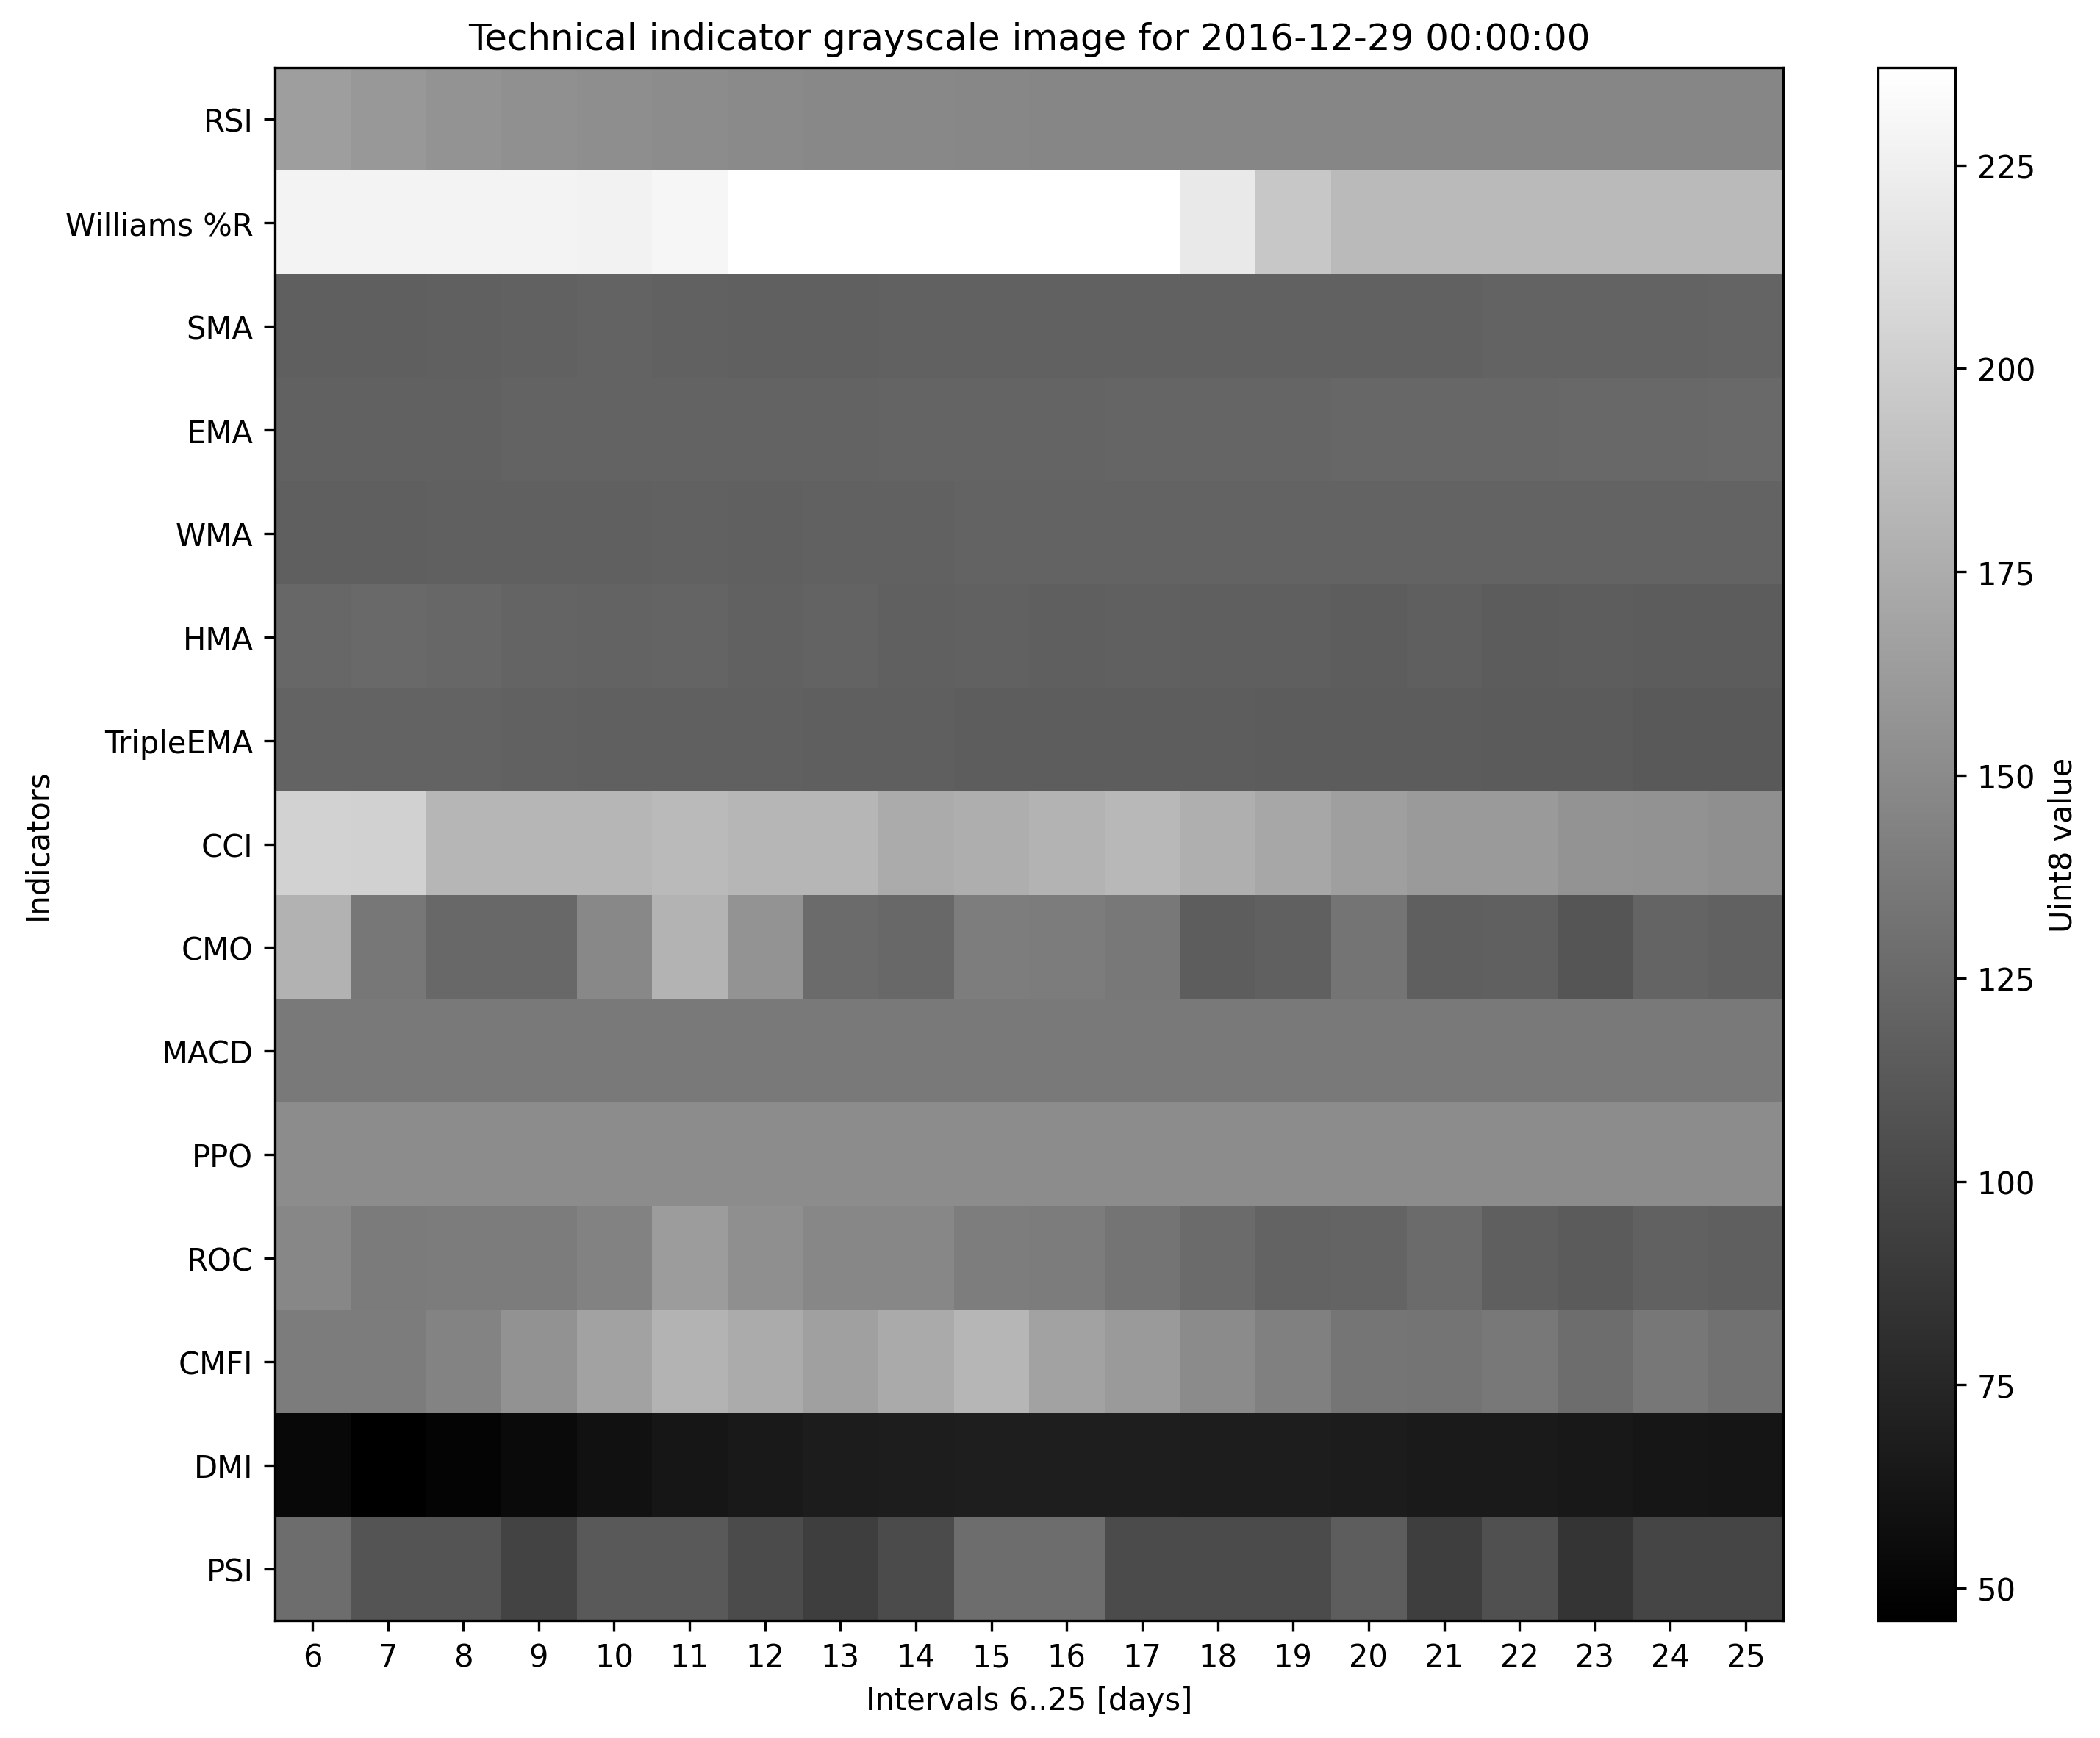
\includegraphics[width=0.85\textwidth]{../figures/Technical_Indicator.png}
	\caption{Example of a technical–only grayscale image ($15 \times 20$). The vertical axis shows the fifteen technical indicators, and the horizontal axis lists lookback windows from six to twenty–five days.}
	\label{fig:tech_only_image}
\end{figure}

Figure~\ref{fig:tech_macro_image} illustrates the combined representation, where the five macroeconomic rows are appended beneath the technical indicators to form a $20 \times 20$ image.


\begin{figure}[H]
	\centering
	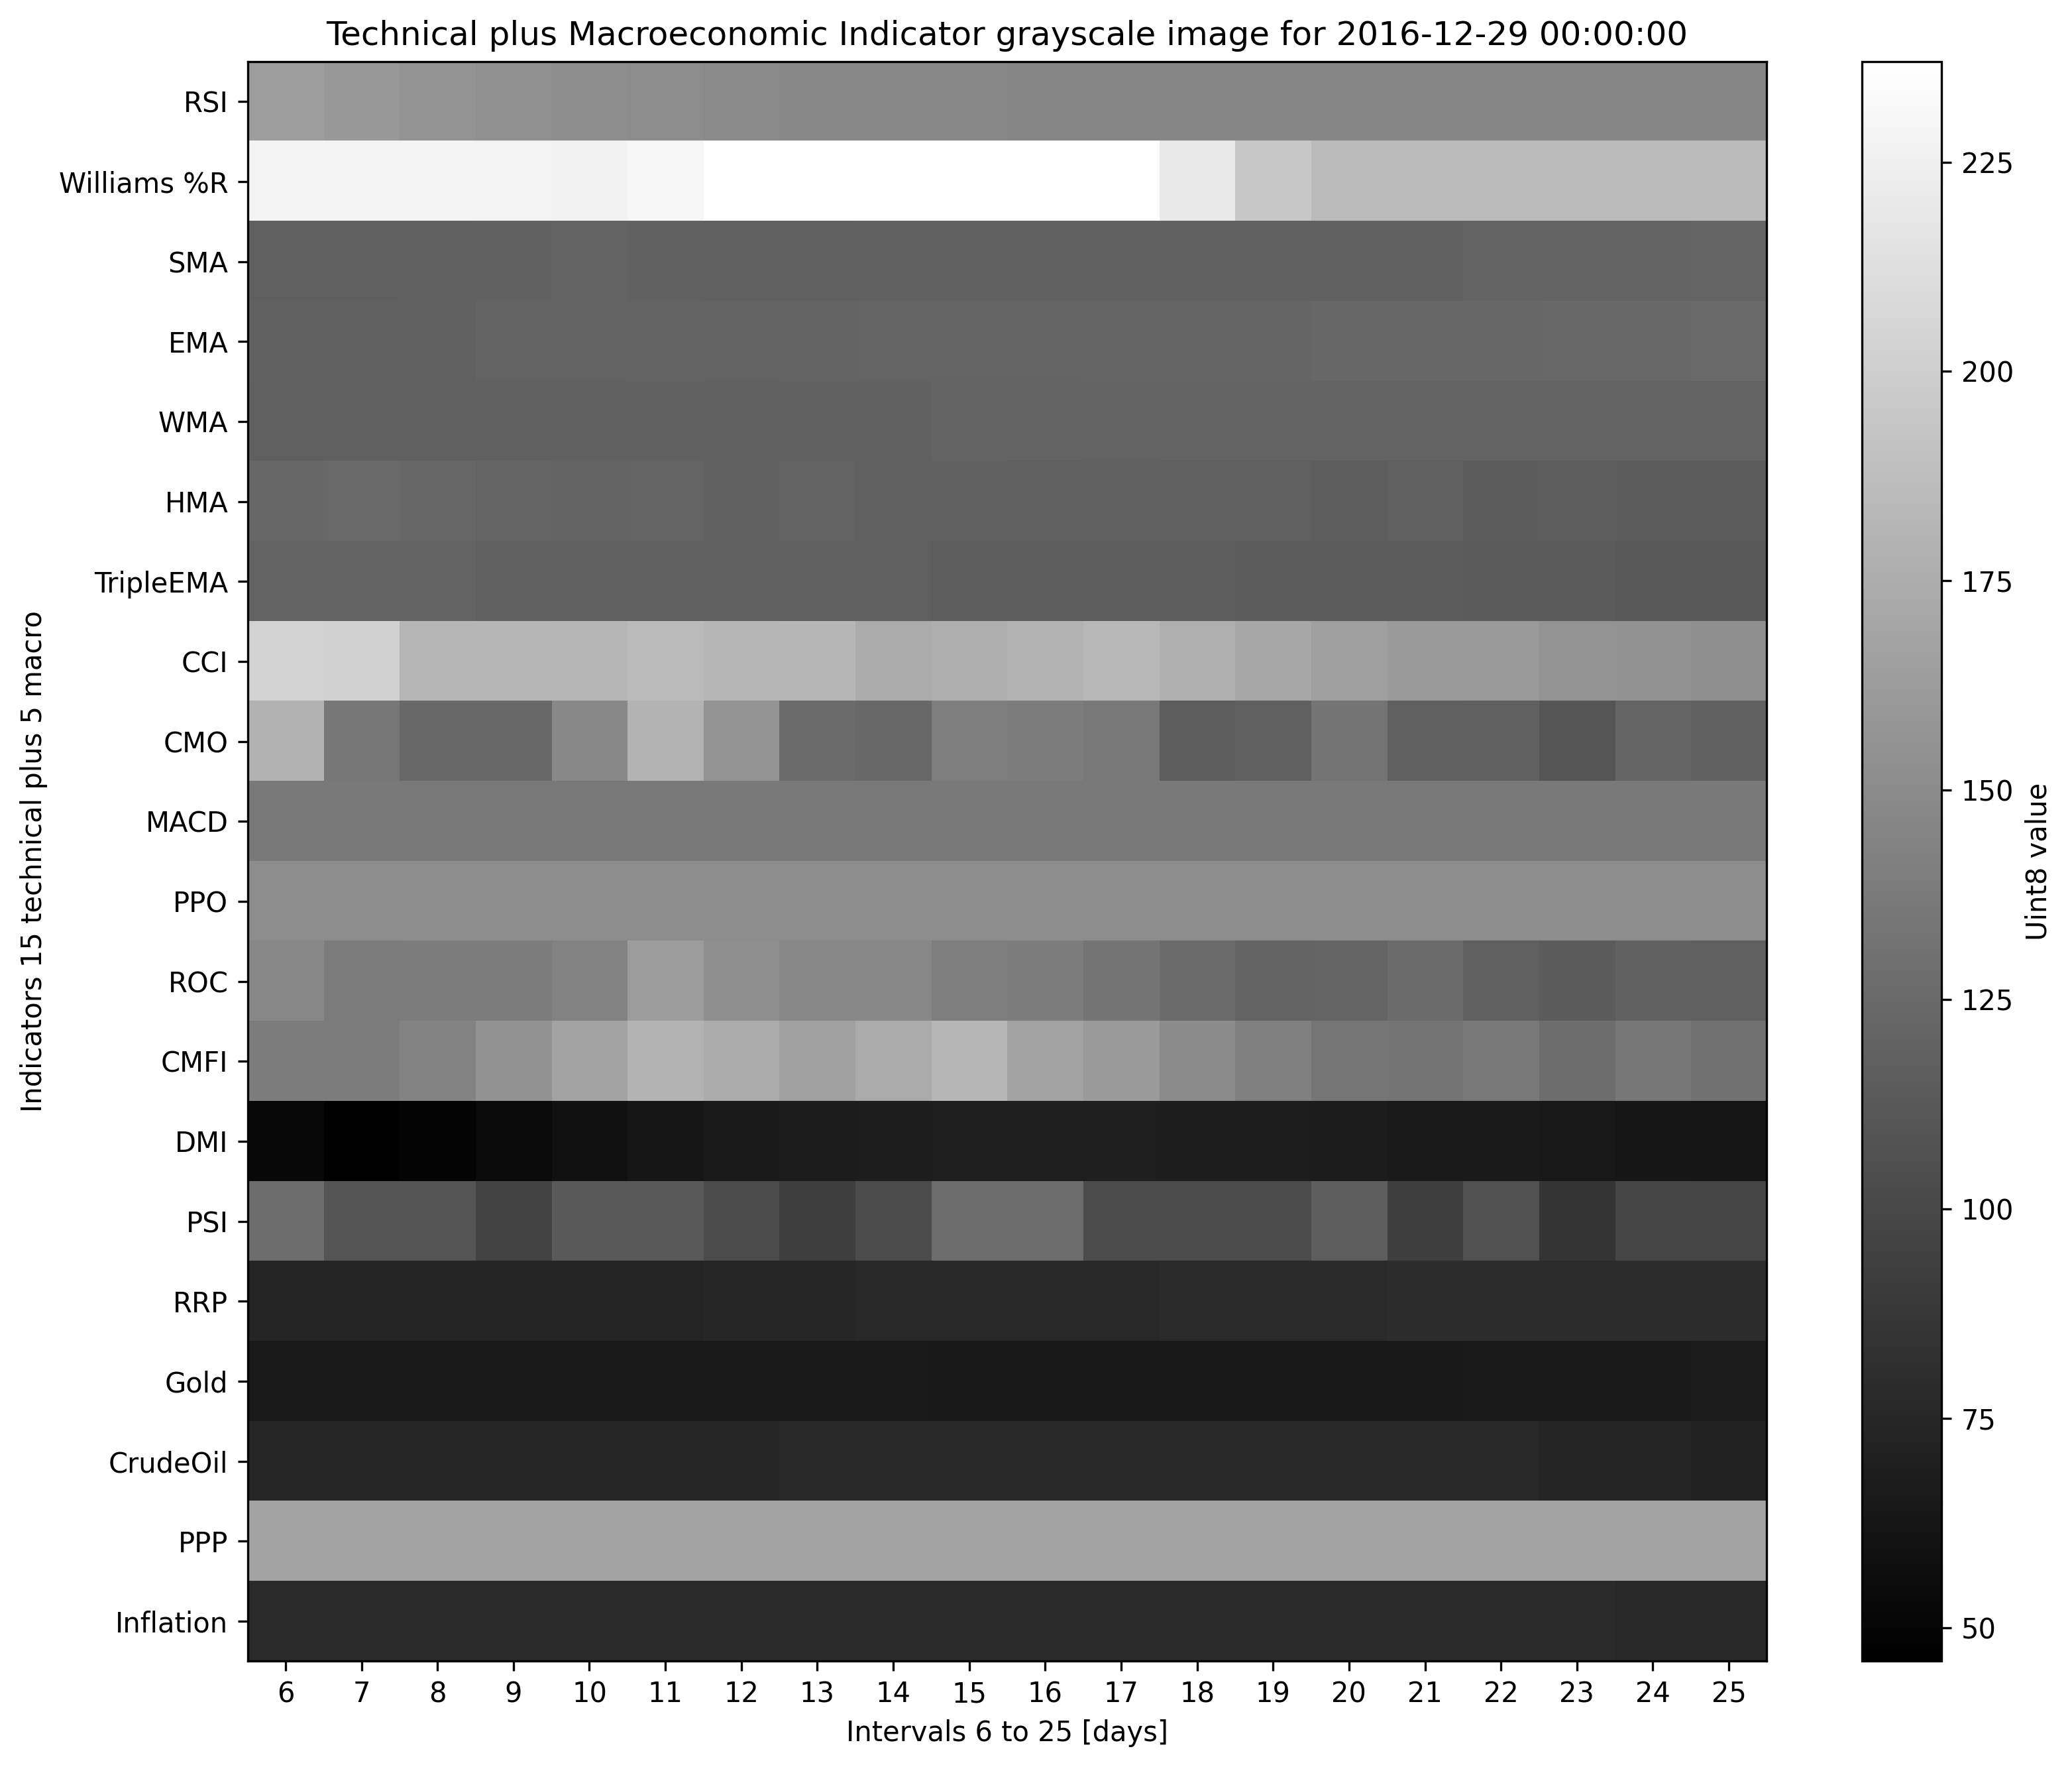
\includegraphics[width=0.85\textwidth]{../figures/CombinedTechandMacro.png}
	\caption{Combined technical and macroeconomic grayscale image ($20 \times 20$). Rows 16–20 contain RRP, Gold, CrudeOil, PPP, and Inflation, aligned to the same set of lookback windows.}
	\label{fig:tech_macro_image}
\end{figure}

In summary, the two representations show how normalized and quantized indicator values are translated into grayscale images. CNN--TIC uses a $15 \times 20$ technical-only image, while CNN--MIC uses a $20 \times 20$ image with additional macroeconomic context. These two image forms serve as input representations for the comparison of the baseline and proposed CNN models.

\subsection{Model Training}
\label{subsec:model-training}

This stage trains two convolutional models under identical settings to allow a fair comparison between the technical-only baseline and the combined technical–macroeconomic approach. The baseline model, CNN--TIC, receives a $15 \times 20$ grayscale image that encodes only the technical indicators. The proposed model, CNN--MIC, refers to a Convolutional Neural Network with Macroeconomic-Integrated Channels. It receives a $20 \times 20$ image where the technical indicators and the macroeconomic series are integrated into a single representation.


\begin{figure}[H]
	\centering
	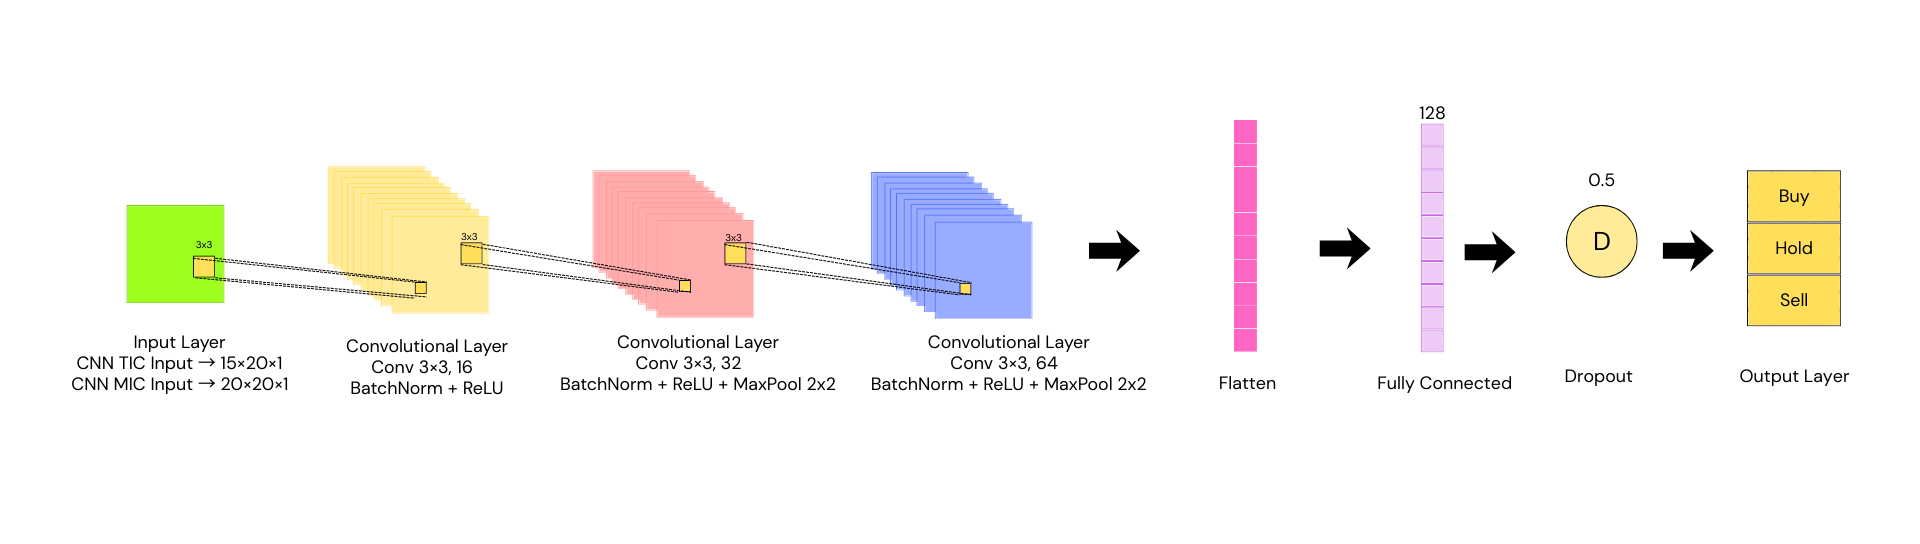
\includegraphics[width=1\textwidth]{../figures/CNN_Architecture.png}
	\caption{SmallCNN\_BN architecture used for both CNN--TIC and CNN--MIC. The network applies three convolutional blocks with batch normalization and ReLU, followed by flattening, a fully connected layer with 128 units, dropout, and a three-unit softmax output.}
	\label{fig:smallcnn-architecture}
\end{figure}

\paragraph{Architecture}

The architecture follows the design principles of earlier image-based trading systems such as CNN--TIC, which showed that shallow convolutional structures are effective for indicator-based images. In this study, the input images are much smaller than those used in standard vision applications. The technical-only images measure $15 \times 20$, and the combined images measure $20 \times 20$. Because of these constraints, deeper architectures and standard vision backbones are unsuitable.

To address this, a compact model called \textbf{SmallCNN\_BN} was constructed. The model adapts the general ideas demonstrated in prior CNN trading literature but is redesigned to match the spatial layout of the technical and macroeconomic representations. The objective is to provide enough capacity to detect local spatial patterns while controlling the risk of overfitting.

The feature extractor consists of three sequential convolutional blocks:

\begin{itemize}
	\item Block 1: Conv($3 \times 3$, 16 filters), BatchNorm, ReLU.
	\item Block 2: Conv($3 \times 3$, 32 filters), BatchNorm, ReLU, MaxPool($2 \times 2$).
	\item Block 3: Conv($3 \times 3$, 64 filters), BatchNorm, ReLU, MaxPool($2 \times 2$).
\end{itemize}

The output of the convolutional blocks is flattened and passed into a fully connected layer with 128 units and ReLU activation. A dropout layer (probability $0.5$) reduces overfitting. The final linear layer outputs three logits corresponding to the Buy, Hold, and Sell classes, followed by a softmax to produce class probabilities.

\paragraph{Training procedure}

Both models use the same training configuration to isolate the effect of the input representation. Weighted cross entropy is used as the loss function with a label smoothing factor of $0.05$. Class weights are computed from the training split using inverse class frequency to reduce the effect of strong class imbalance in the Buy and Sell categories.

Training uses the AdamW optimizer with a learning rate of $10^{-3}$, weight decay of $10^{-4}$, batch size of $128$, and a cosine annealing learning rate schedule. Each model is trained for $50$ epochs. For every cross-validation fold, the checkpoint with the highest validation macro F1 is retained.

\paragraph{Decision rule}

During inference, the predicted class for day $t$ is obtained by an argmax over the softmax probabilities:

\[
\hat{y}_t = \arg\max_{c \in \{\text{Buy, Hold, Sell}\}} \hat{p}_{t,c}.
\]

The class labels are then mapped into the trading actions used by the financial evaluation procedure described in Algorithm~\ref{alg:financial-evaluation}. This produces a sequence of actionable signals that are passed into the backtesting stage of the framework.

\begin{algorithm}[H]
	\footnotesize
	\caption{FinancialEvaluation}
	\label{alg:financial-evaluation}
	\begin{algorithmic}[1]
		\Procedure{FINANCIALEVALUATION}{}
		\State $balance = 10000$ PHP
		\State $bought\_amount = 0$
		\State $commission = 50$ PHP
		\State $take\_profit = 10\%$
		\State $stop\_loss = 1\%$
		\ForAll{$(price, predicted\_action)$ in $testDataset$}
		\If{$bought\_amount \neq 0$}
		\If{$price > take\_profit\_price$}
		\State $balance = bought\_amount * take\_profit\_price - commission$
		\State $bought\_amount = 0$
		\EndIf
		\If{$price < stop\_loss\_price$}
		\State $balance = bought\_amount * stop\_loss\_price - commission$
		\State $bought\_amount = 0$
		\EndIf
		\EndIf
		\If{$predicted\_action == BUY$ and $balance \neq 0$}
		\State $bought\_amount = (balance - commission) / price$
		\State $balance = 0$
		\State $take\_profit\_price = price * (1.0 + take\_profit / 100)$
		\State $stop\_loss\_price = price * (1.0 - stop\_loss / 100)$
		\EndIf
		\If{$predicted\_action == SELL$ and $bought\_amount \neq 0$}
		\State $balance = bought\_amount * price - commission$
		\State $bought\_amount = 0$
		\EndIf
		\EndFor
		\State \Return $balance$
		\EndProcedure
	\end{algorithmic}
\end{algorithm}


\subsection{Model Evaluation}
\label{subsec:model-eval}

This stage evaluates the models along two dimensions: classification accuracy and trading performance. The first set of metrics measures how well the models predict the Buy, Hold, and Sell classes. The second set measures how these predictions translate into financial outcomes when executed under a fixed trading strategy.

\paragraph{Classification metrics}

Accuracy and macro F1 are used to assess classification performance. These metrics are computed for every fold during cross-validation and averaged to obtain a stable estimate of model behavior. After training on the full training pool, the same metrics are computed on the test period to evaluate generalization.


\paragraph{Trading metrics}

To assess economic relevance, the predicted labels are converted into trading actions using the rules defined in Algorithm~\ref{alg:financial-evaluation}. The evaluation uses fixed parameters for both models to ensure a fair comparison. A Buy signal opens a long position on the next market open. A Sell signal closes any existing position. A Hold signal maintains the current position. Each transaction includes a 50-peso commission. The strategy applies a take-profit threshold of 10 percent and a stop-loss threshold of 1 percent relative to the entry price.

\paragraph{Output}

The procedure produces yearly returns, mean annual return, and final equity for the test period. These metrics allow the framework to determine whether improvements in representation lead to measurable gains in trading performance under identical simulation settings.

 %methodology
\chapter{Results and Discussion}
\label{chap:results}

\section{Performance Evaluation Metrics}

To measure the performance of each model, the study used the same metrics used from previous works of CNN--TIC studies for both classification and financial evaluation \cite{maratkhan2021deep}. For classification performance, validation accuracy, test accuracy, and macro F1-score were used. These metrics are important to measure not only the total number of correct predictions, but also the balance of the model's performance in the Buy, Hold, and Sell classes.

For financial evaluation, final equity, mean annual return, and standard deviation of annual return were used. Final equity shows the total amount obtained after applying the trading strategy in the test period. The mean annual return measures the typical annual return of the strategy, while the standard deviation refers to the degree of variability of returns across years. In this way, the models are evaluated not only as classifiers but also as systems used in actual trading simulations.

\section{Implementation Details and Training Protocol}
All experiments in this study were performed on a workstation running Ubuntu 24.04.3 LTS. The system has an Intel Core i7-14700 processor, running at up to 5.4~GHz, 62~GB of system memory, and an NVIDIA GeForce RTX 4070 Ti GPU with 12~GB VRAM. 


All experiments in this chapter were conducted using the same preprocessing pipeline, labeling strategy, image construction procedure, and trading simulation rules presented in Chapter 3. The baseline model is CNN--TIC, which uses only technical indicators as input representation, while the proposed model CNN--MIC extends this representation by including macroeconomic indicators.

The two models were evaluated under five validation schemes, namely, Chronological Holdout Validation with Stratified K-Fold, Expanding-Window Walk-Forward Validation, Nested Walk-Forward Validation, Blocked Cross-Validation, and Blocked Cross-Validation with Partial Undersampling. Using multiple validation schemes is important to measure whether the performance of each model remains robust across different evaluation settings.

\section{Experimental Setups}
The experiments were organized into three major asset groups, blue-chip stocks, penny stocks, and cryptocurrency. For blue-chip stocks, Ayala Corporation (AC), Jollibee Foods Corporation (JFC), and SM Investments Corporation (SMI) were examined. For penny stocks, these included PH Resorts Group (PHR), United Paragon Mining Corporation (UPM), and Araneta Properties (ARA). Lastly for cryptocurrency, Bitcoin (BTC), Litecoin (LTC), and XRP were examined.

\subsection{Experiment 1: Comparing CNN--TIC and CNN--MIC with Different Validation Schemes}

The first experiment was conducted to examine how the performance of CNN--TIC and CNN--MIC differed across the five validation schemes used in the study. This experiment examined how the inclusion of macroeconomic indicators affected validation performance across different evaluation setups.

\subsection{Experiment 2: Benchmarking Test Classification and Financial Performance}

The second experiment was conducted to compare the performance of two models on out-of-sample data using accuracy, Macro F1-score, and financial metrics such as annualized return. This experiment aimed to determine how the inclusion of macroeconomic indicators affected both predictive performance and trading performance.

\subsection{Experiment 3: SHAP-Based Interpretation of CNN--MIC Across Validation Schemes}

The third experiment was conducted to interpret the behavior of CNN--MIC using SHAP analysis. The main discussion focuses on Ayala Corporation (AC) across the validation schemes, while additional predicted-class SHAP row importance plots for selected assets under BCV-PU are presented in Appendix A.4. Unlike the first two experiments, which compared the numerical performance of CNN--TIC and CNN--MIC across multiple assets and asset groups, this experiment focused on one representative stock in order to examine how feature contribution changes under different validation schemes. The analysis aimed to determine whether the model remained primarily driven by technical indicators across all evaluation settings and to identify which macroeconomic variables provided supporting information in each scheme.


\section{Results and Discussion}
The results in this chapter are organized according to the three experiments presented in the previous section. For the presentation of tables, the validation schemes are abbreviated as CHV-SKF for Chronological Holdout Validation with Stratified K-Fold, EW-WFV for Expanding-Window Walk-Forward Validation, NWFV for Nested Walk-Forward Validation, BCV for Blocked Cross-Validation, and BCV-PU for Blocked Cross-Validation with Partial Undersampling.

\subsection{Experiment 1: Comparison of Validation Performance Across Validation Schemes}

Table~\ref{tab:val_bluechip} to Table~\ref{tab:val_crypto} in Appendix~\ref{app:experiment1_tables} show the validation performance of CNN--TIC and CNN--MIC on the three asset groups. The numerical results show that the effect of adding macroeconomic indicators is not uniform across all assets and validation schemes. Instead, the observed gains vary depending on both the characteristics of the asset and the structure of the validation procedure. This suggests that the contribution of macroeconomic information is conditional rather than universal. To better compare the validation behavior of the two models, the validation accuracy scores were summarized using box plots for each asset.


\begin{center}
	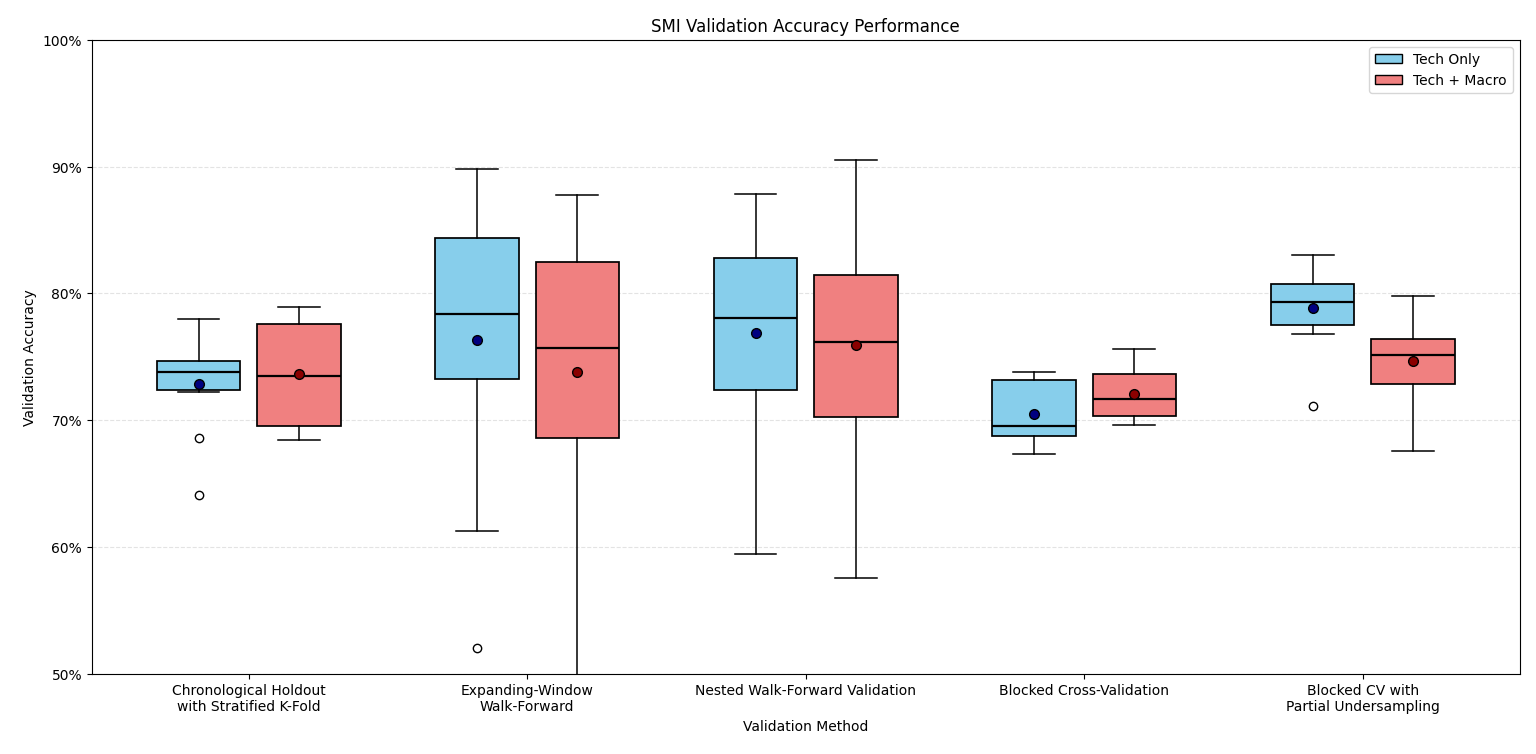
\includegraphics[width=0.8\textwidth]{../figures/SMI_Val.png}\\
	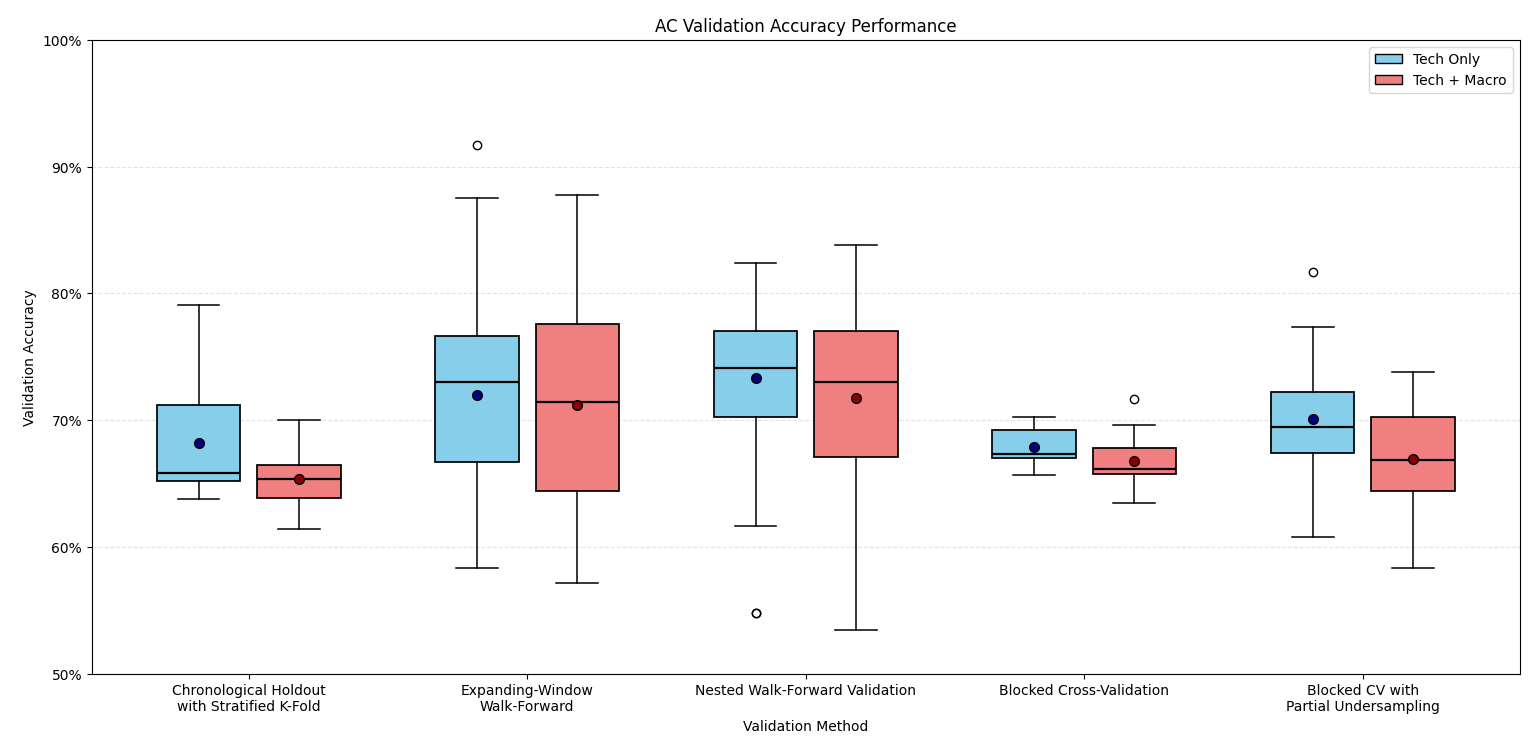
\includegraphics[width=0.8\textwidth]{../figures/AC_Val.png}\\
	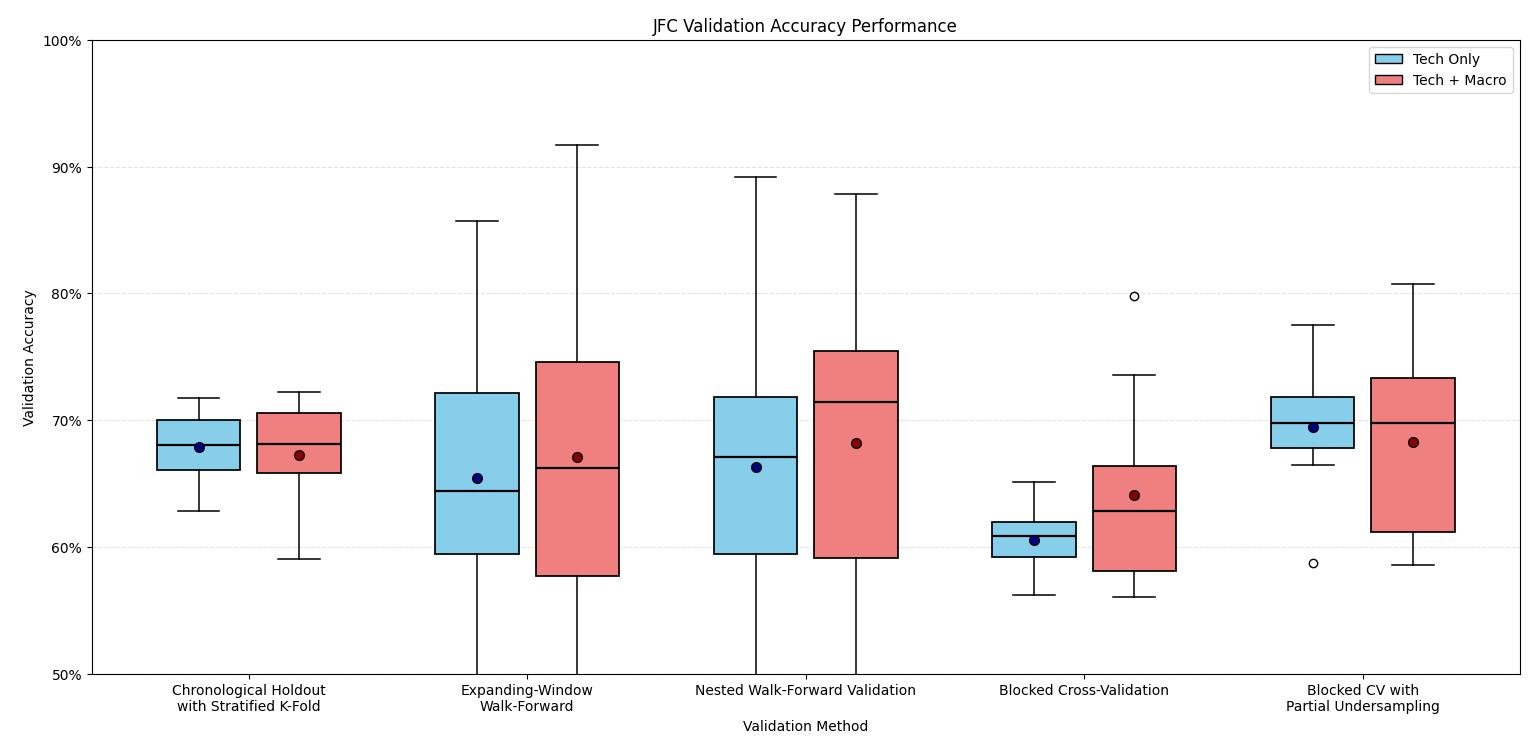
\includegraphics[width=0.8\textwidth]{../figures/JFC_Val.png}
	
	\captionof{figure}{Validation accuracy performance of CNN--TIC and CNN--MIC across selected blue-chip stocks}
	\label{fig:val_bluechip_boxplots}
\end{center}

Figure~\ref{fig:val_bluechip_boxplots} shows the validation accuracy performance of CNN--TIC and CNN--MIC across SMI, AC, and JFC. For the blue-chip group, the results were mixed. CNN--MIC was more competitive in selected settings for AC and JFC, particularly in Expanding-Window Walk-Forward and some Blocked Cross-Validation-based schemes. However, CNN--TIC remained stronger in several Nested Walk-Forward Validation and Blocked Cross-Validation with Partial Undersampling results, especially for SMI. This indicates that macroeconomic integration does not consistently improve validation performance for large-cap assets.

\begin{center}
	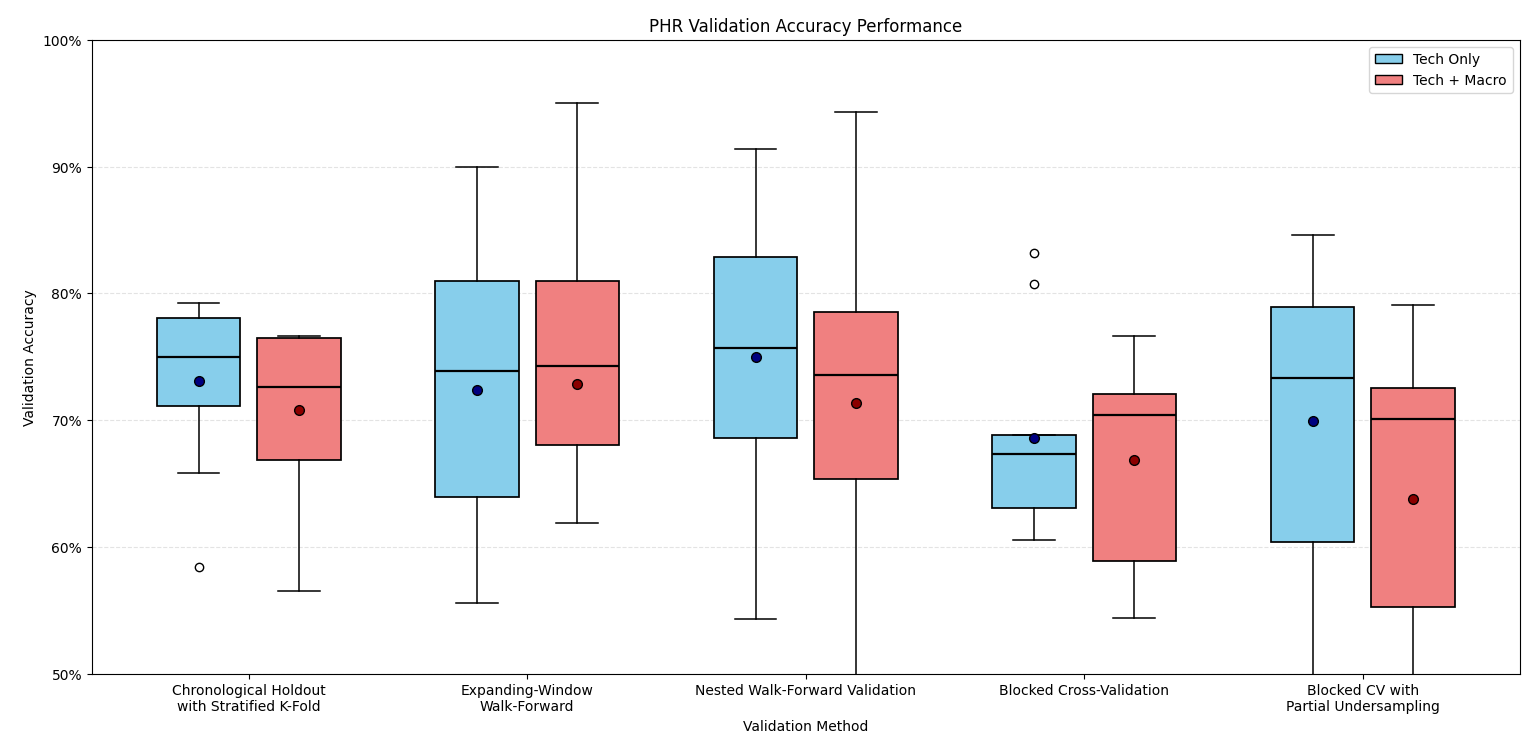
\includegraphics[width=0.8\textwidth]{../figures/PHR_Val.png}
	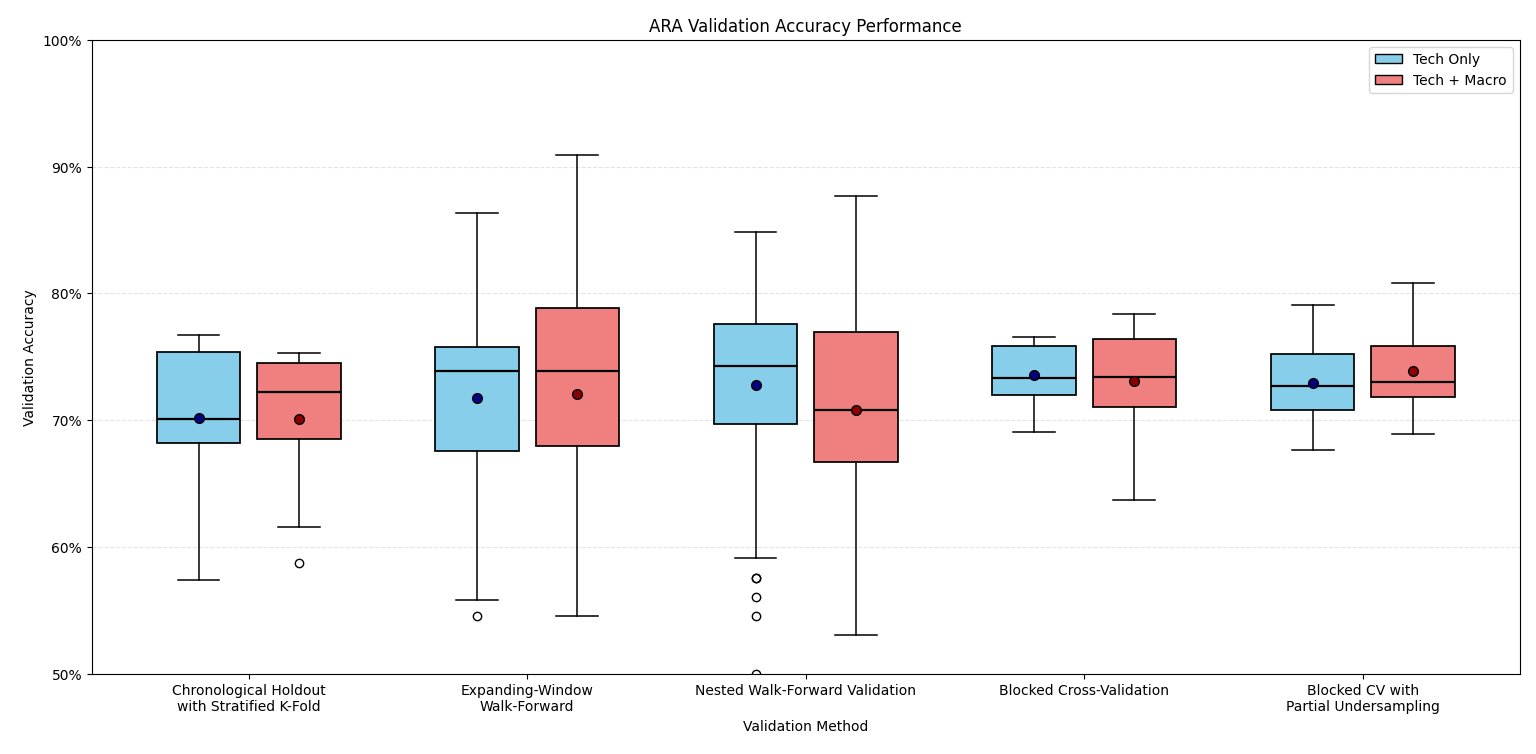
\includegraphics[width=0.8\textwidth]{../figures/ARA_Val.png}
	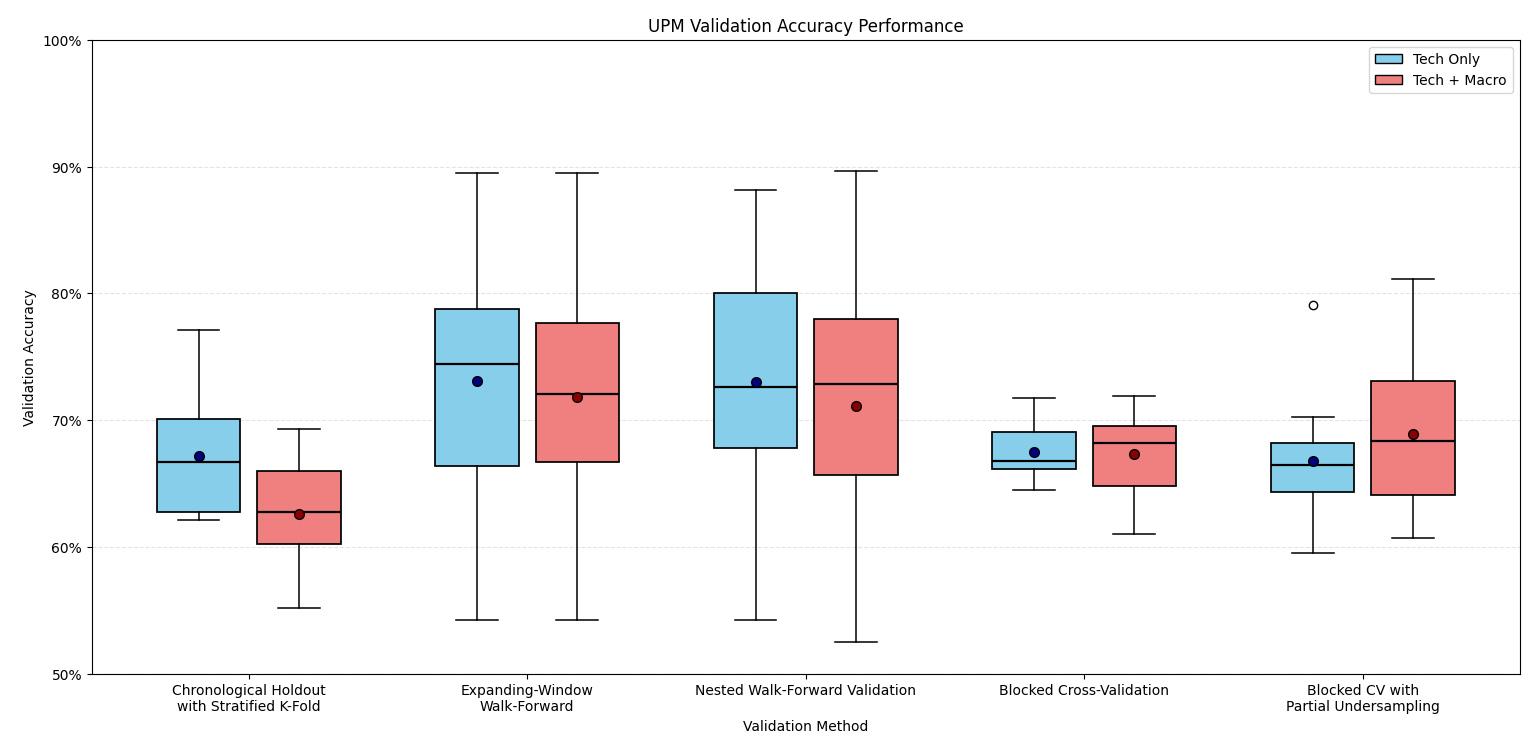
\includegraphics[width=0.8\textwidth]{../figures/UPM_Val.png}
	
	\captionof{figure}{Validation accuracy performance of CNN--TIC and CNN--MIC across selected penny stocks}
	\label{fig:val_penny_boxplots}
\end{center}

Figure~\ref{fig:val_penny_boxplots} shows the validation accuracy performance of CNN--TIC and CNN--MIC across PHR, ARA, and UPM. For penny stocks, CNN--TIC remained more competitive in UPM and PHR across most schemes. In contrast, CNN--MIC showed its clearest advantage in ARA, particularly in selected validation settings. These results suggest that the effect of macroeconomic indicators in low-priced equities is also selective rather than uniform.

\begin{center}
	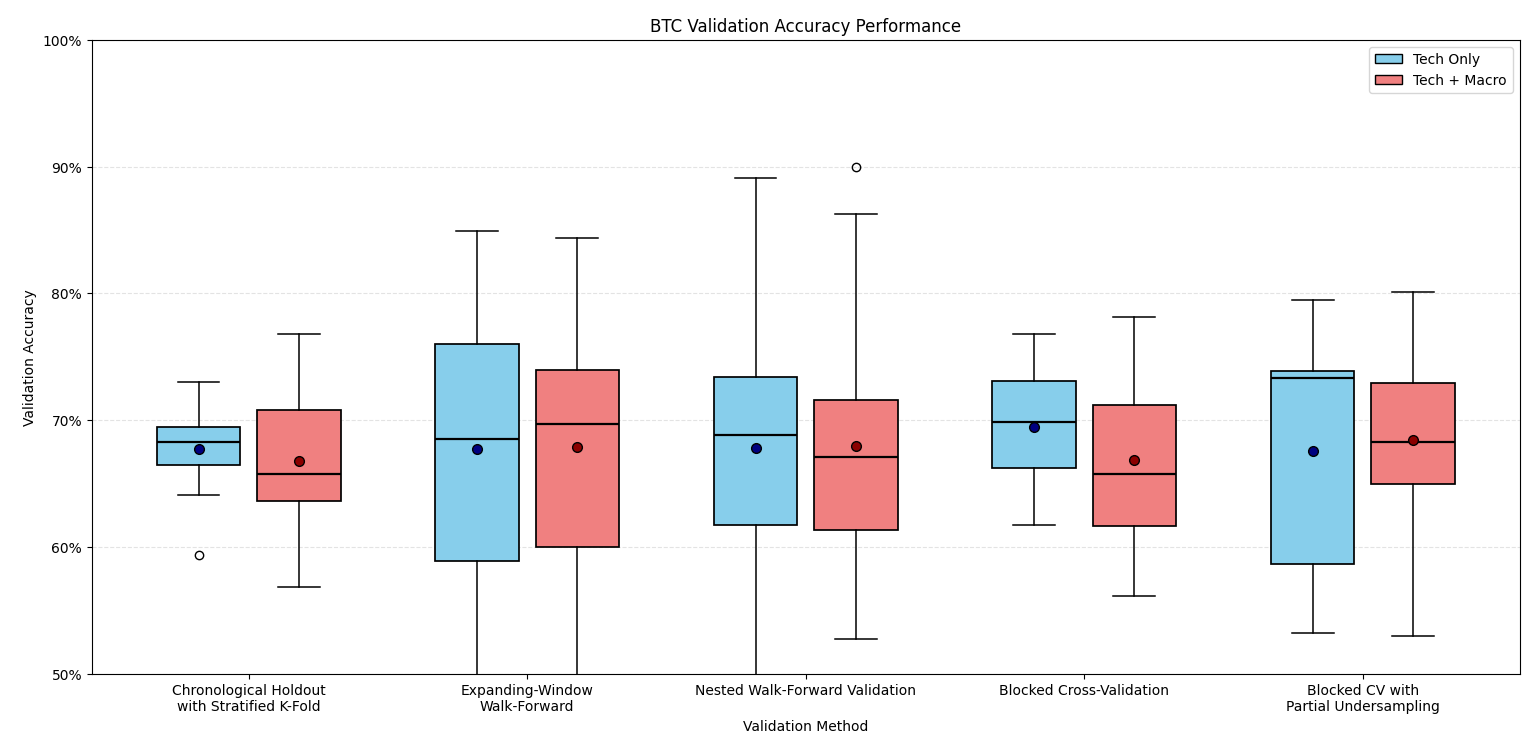
\includegraphics[width=0.8\textwidth]{../figures/BTC_Val.png}
	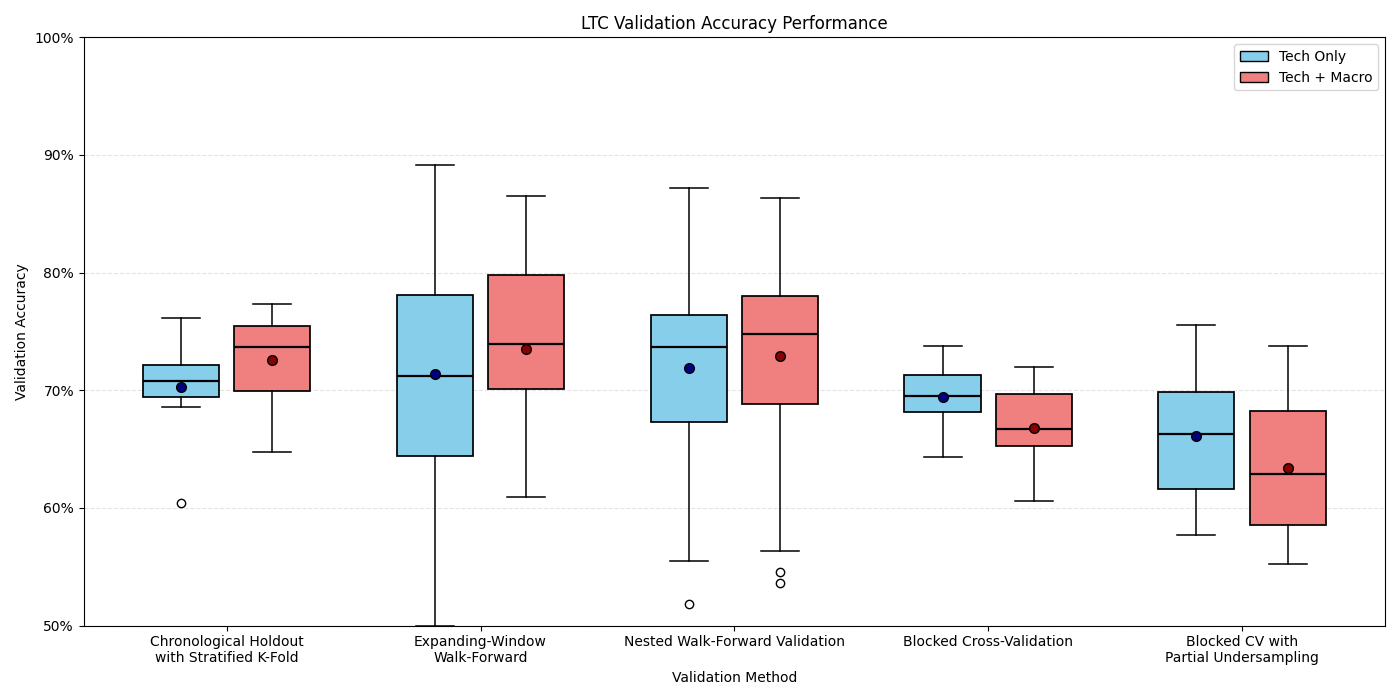
\includegraphics[width=0.8\textwidth]{../figures/LTC_Val.png}
	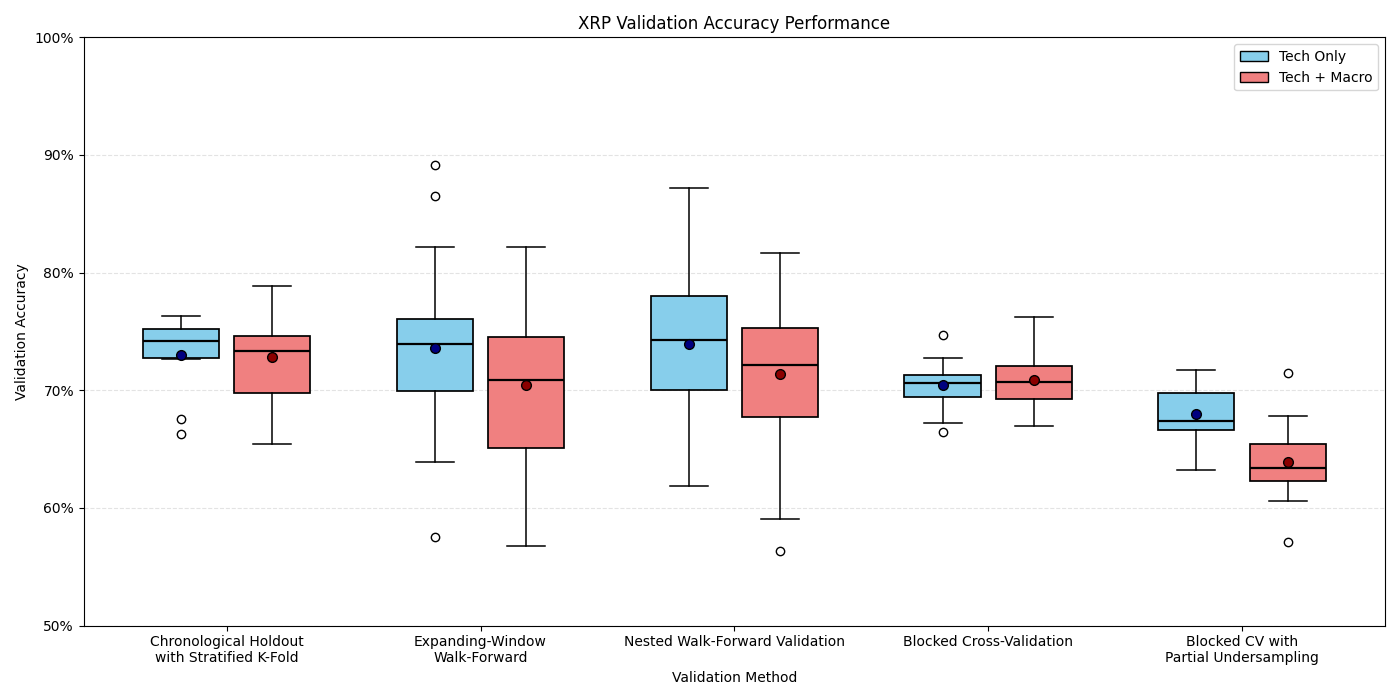
\includegraphics[width=0.8\textwidth]{../figures/XRP_Val.png}
	
	\captionof{figure}{Validation accuracy performance of CNN--TIC and CNN--MIC across selected cryptocurrency assets}
	\label{fig:val_crypto_boxplots}
\end{center}

Figure~\ref{fig:val_crypto_boxplots} shows the validation accuracy performance of CNN--TIC and CNN--MIC across BTC, LTC, and XRP. For cryptocurrencies, CNN--MIC showed clearer gains in BTC and LTC under selected validation schemes, particularly in Expanding-Window Walk-Forward and Nested Walk-Forward Validation. However, CNN--TIC remained stronger for XRP across most settings. Among the three asset groups, the cryptocurrency group shows the most visible but still asset-specific benefit from macroeconomic integration.



\subsection{Experiment 2: Comparison of Test Classification and Financial Performance}
This experiment compares CNN--TIC and CNN--MIC not only as classifiers, but also as Buy, Hold, and Sell trading systems. In the financial evaluation, each predicted class is treated as a trading signal and executed using the same backtesting rules described in Algorithm~\ref{alg:financial-evaluation}. The comparison therefore measures whether the Buy, Hold, and Sell decisions produced by the technical-only model or the macroeconomic-integrated model lead to stronger portfolio outcomes.

It is important to distinguish classification performance from financial performance. Accuracy measures how often the predicted class matches the ground-truth label. However, profitability depends on the timing, direction, and economic consequence of each predicted action. A model may obtain higher accuracy by correctly predicting many Hold instances, but still miss fewer Buy or Sell signals that have larger effects on portfolio value. 
Similarly, a model with lower accuracy may still generate better financial results if its correct predictions occur near more profitable entry and exit points. This distinction is important in trading systems because economic value is affected not only by predictive correctness, but also by transaction costs, class imbalance, return magnitude, and the sequence of executed trades \cite{moosa2015directional,fischer2021feature,ozbayoglu2020deep}. Therefore, this study evaluates the models using both classification metrics and trading metrics.

Tables~\ref{tab:test_bluechip} to~\ref{tab:fin_crypto} in Appendix~\ref{app:experiment2_tables} present the complete out-of-sample classification and financial performance values of CNN--TIC and CNN--MIC. 
The classification results show how well the models predicted the Buy, Hold, and Sell labels on unseen data. The financial results show whether these predicted actions translated into higher final equity under the fixed trading simulation. This distinction is necessary because a higher test accuracy does not automatically imply a more profitable strategy. 

In trading, the value of a prediction depends on when the signal occurs and how much price movement follows after the executed action \cite{moosa2015directional,fischer2021feature}. To make the comparison clearer, the test accuracy and final equity results were summarized using grouped bar charts for each asset group.

The financial comparison is based on the Buy, Hold, and Sell predictions generated by each model. CNN--TIC produces these actions from the technical-only image representation, while CNN--MIC produces the same action classes from the combined technical and macroeconomic image representation. Both models are evaluated with identical starting capital, commission, take-profit, and stop-loss rules.

\begin{center}
	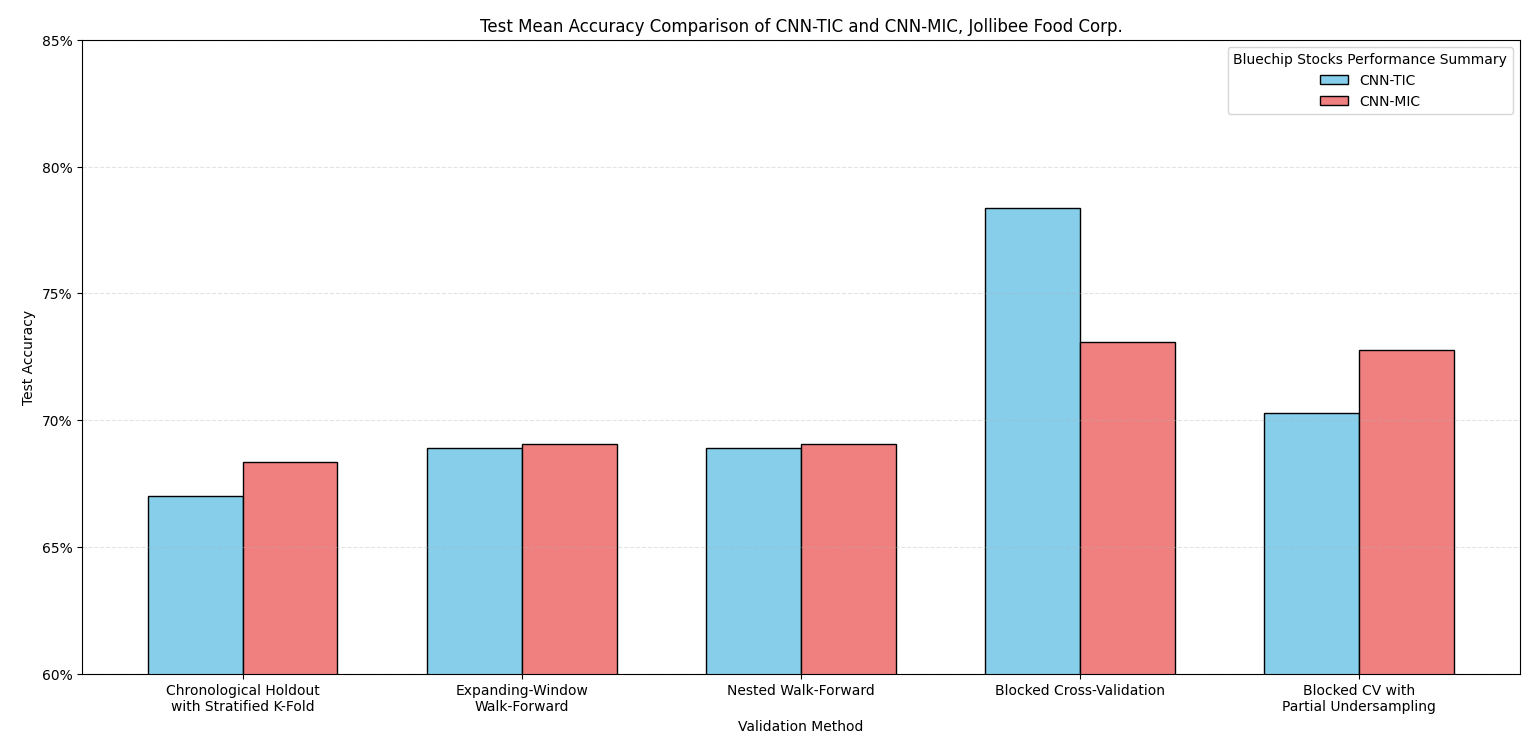
\includegraphics[width=0.8\textwidth]{../figures/JFC_TestAccuracy.png}
	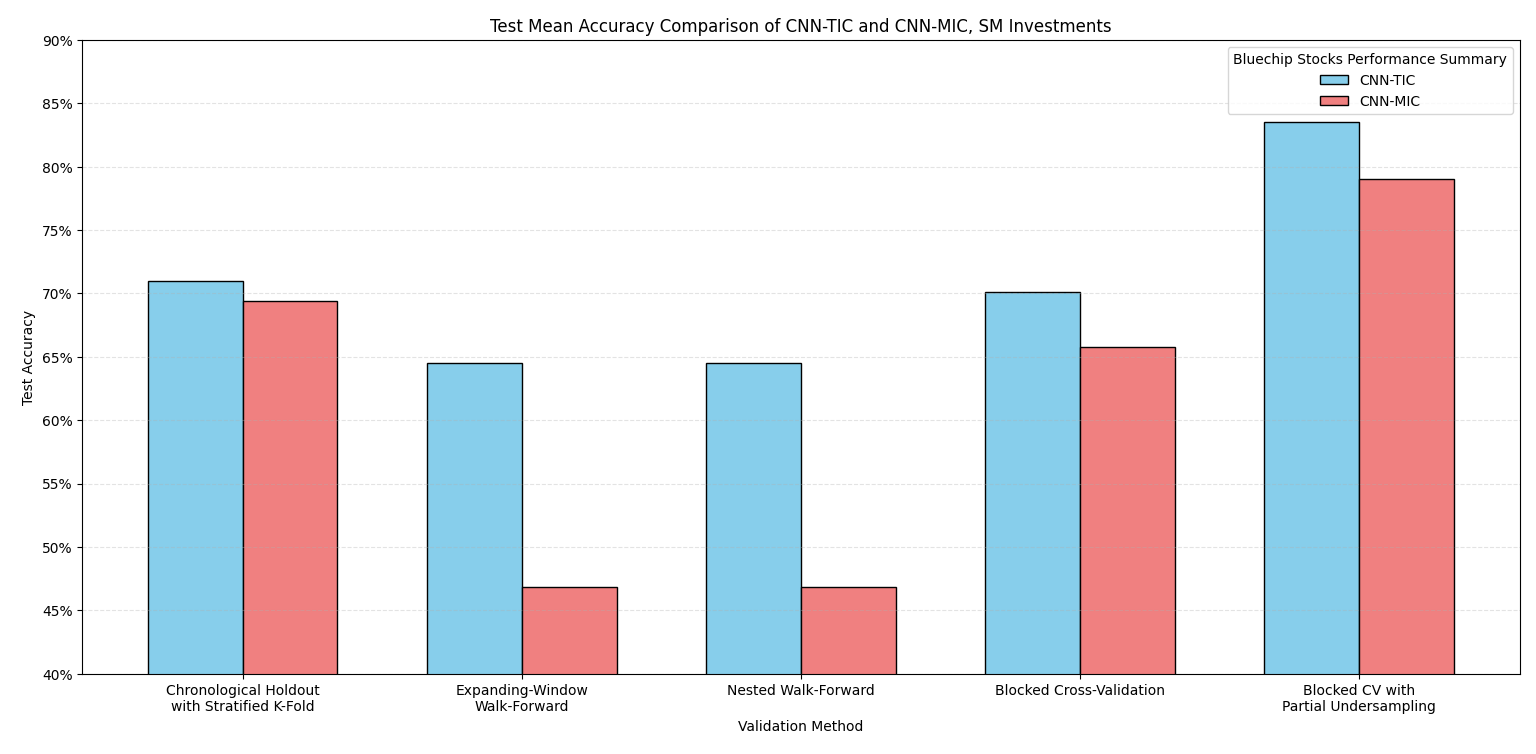
\includegraphics[width=0.8\textwidth]{../figures/SMI_TestAccuracy.png}
	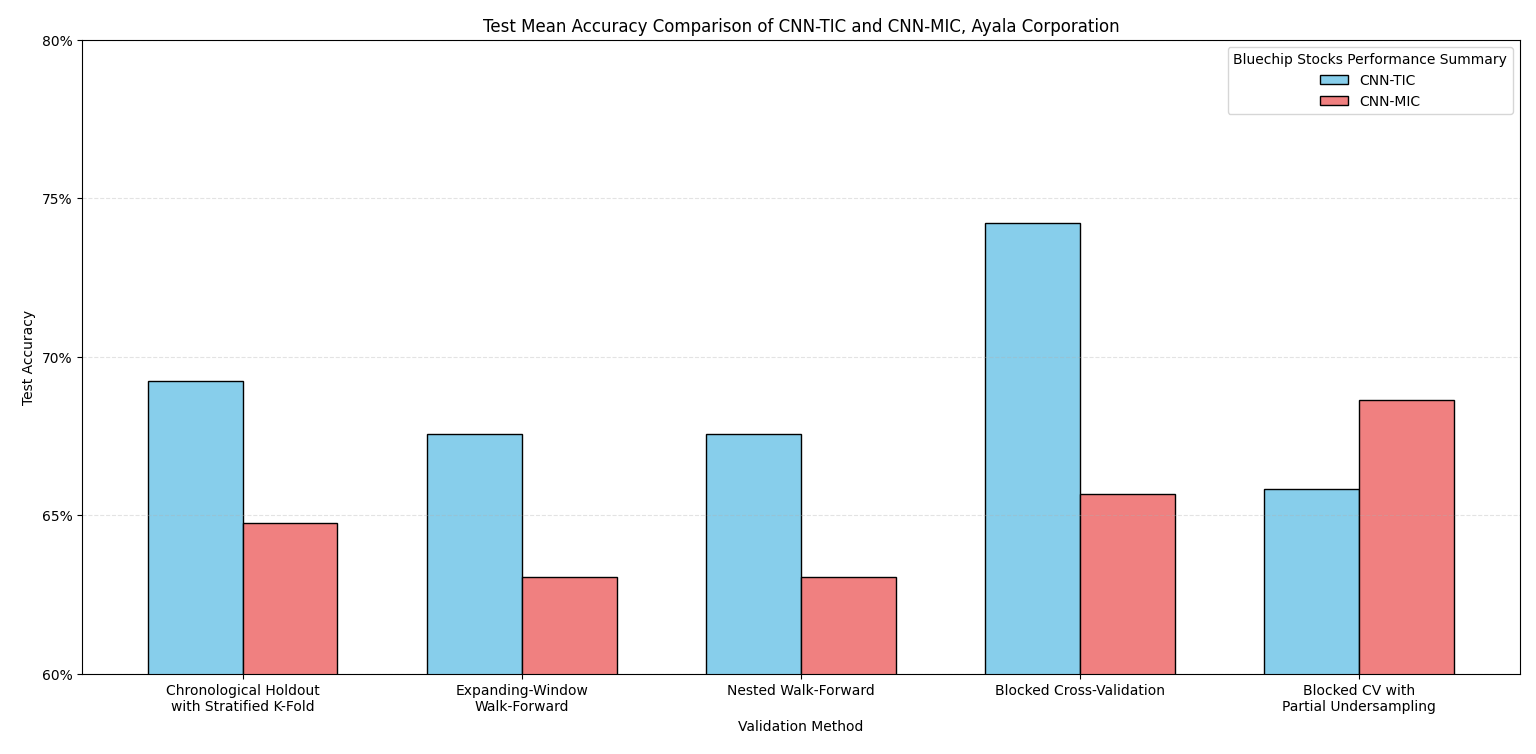
\includegraphics[width=0.8\textwidth]{../figures/AC_TestAccuracy.png}
	
	\captionof{figure}{Test accuracy performance of CNN--TIC and CNN--MIC across selected blue-chip stocks}
	\label{fig:test_bluechip_barplots}
\end{center}

\begin{center}
	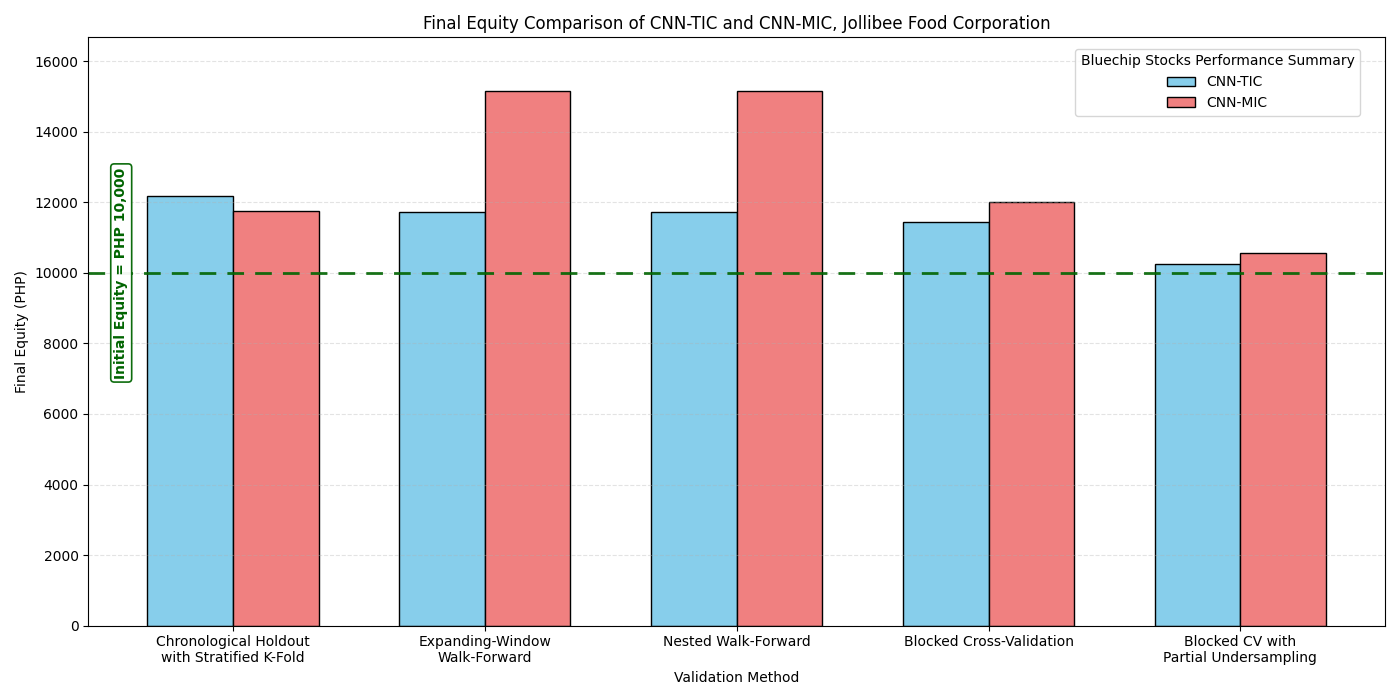
\includegraphics[width=0.8\textwidth]{../figures/JFC_FinancialAccuracy.png}
	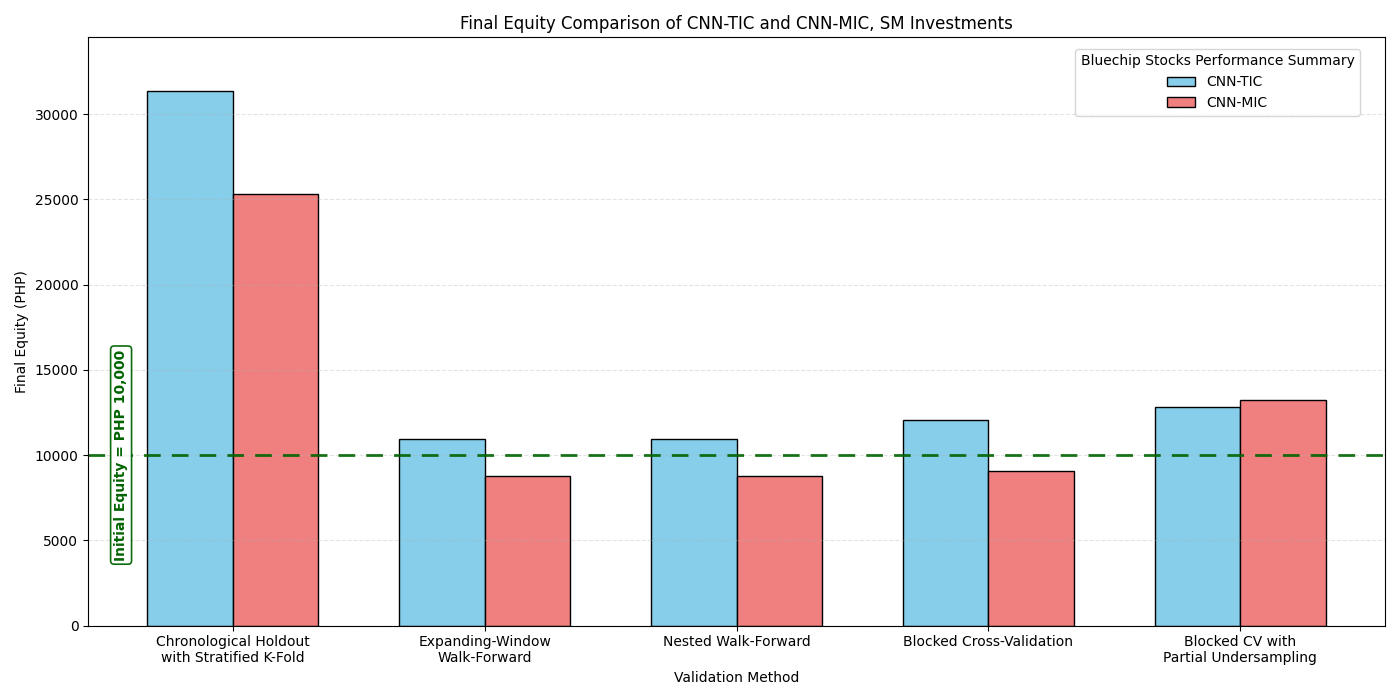
\includegraphics[width=0.8\textwidth]{../figures/SMI_FinancialAccuracy.png}
	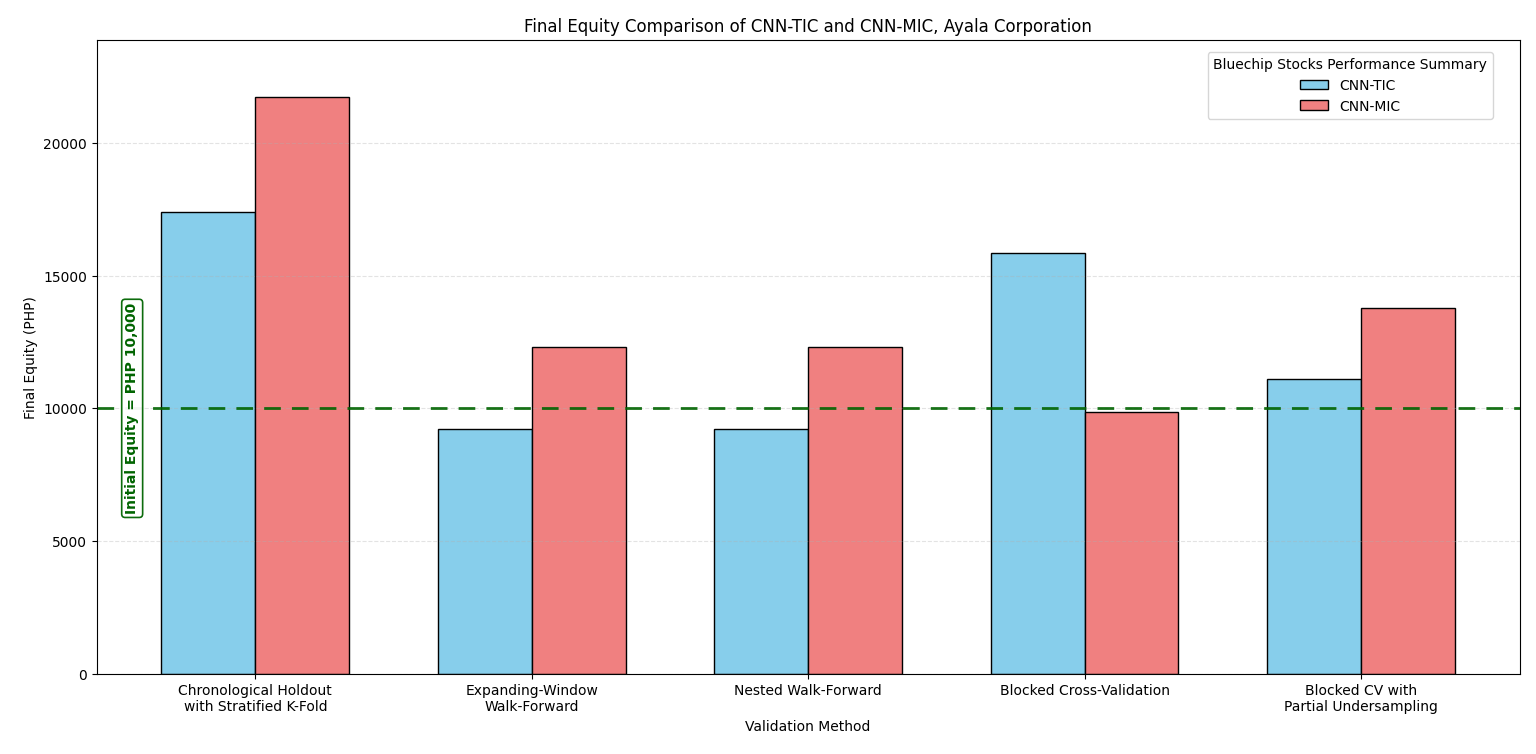
\includegraphics[width=0.8\textwidth]{../figures/AC_FinancialAccuracy.png}
	
	\captionof{figure}{Final equity performance of CNN--TIC and CNN--MIC across selected blue-chip stocks}
	\label{fig:fin_bluechip_barplots}
\end{center}

Figures~\ref{fig:test_bluechip_barplots} and~\ref{fig:fin_bluechip_barplots} show the test accuracy and final equity performance of CNN--TIC and CNN--MIC across the selected blue-chip stocks. Across this group, the out-of-sample classification results remained mixed. CNN--MIC was more competitive for JFC and selected AC settings, while CNN--TIC remained stronger for SMI and several BCV-based results. The financial results followed a similar asset-specific pattern. CNN--MIC produced stronger final equity for AC and selected JFC settings, whereas CNN--TIC remained stronger for SMI in most configurations. This suggests that macroeconomic information can help in selected large-cap cases, but the gains do not transfer consistently across all blue-chip assets.

\begin{center}
	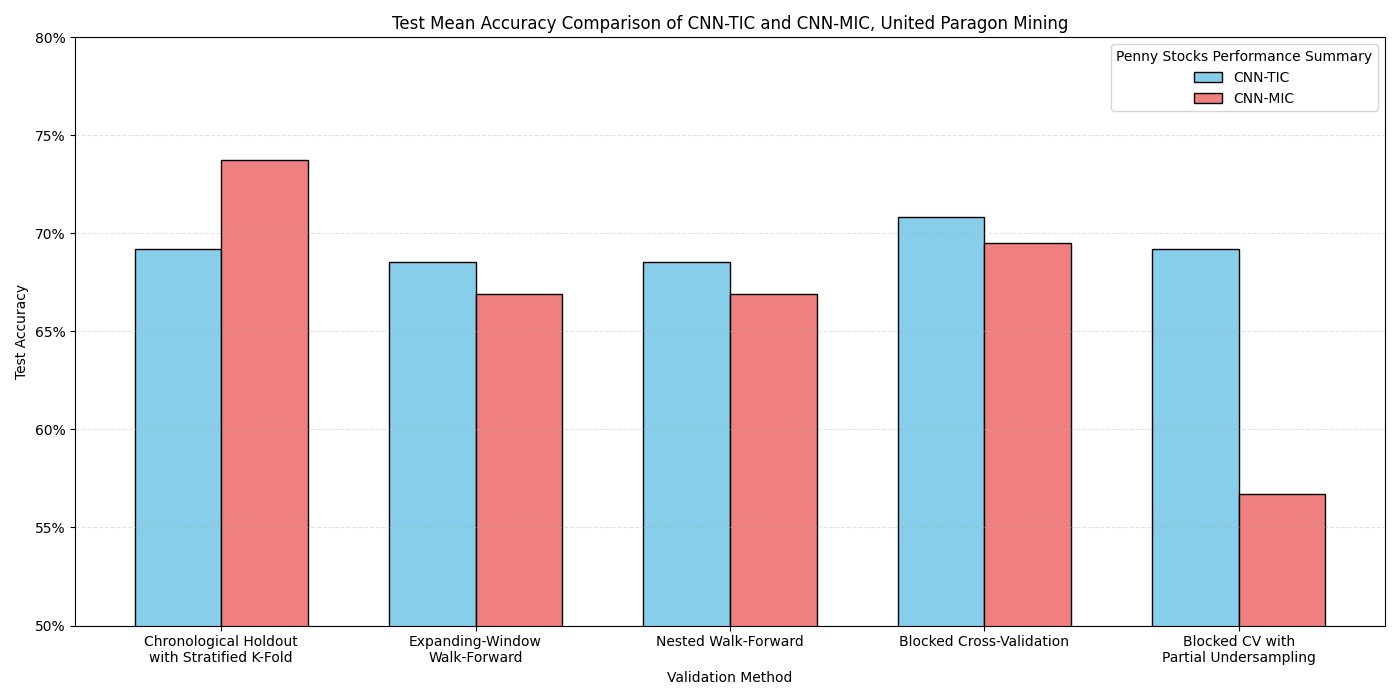
\includegraphics[width=0.8\textwidth]{../figures/UPM_TestAccuracy.png}
	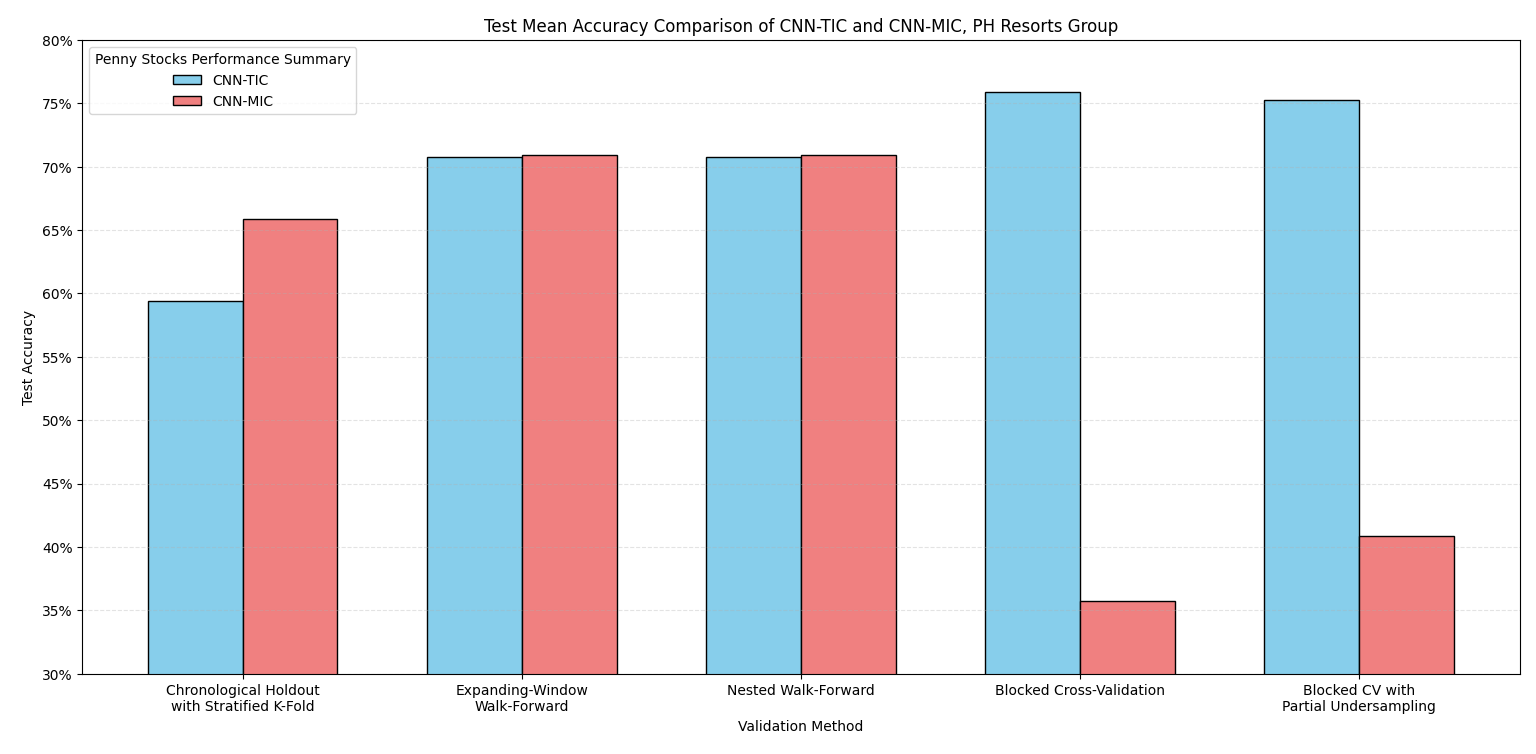
\includegraphics[width=0.8\textwidth]{../figures/PHR_TestAccuracy.png}
	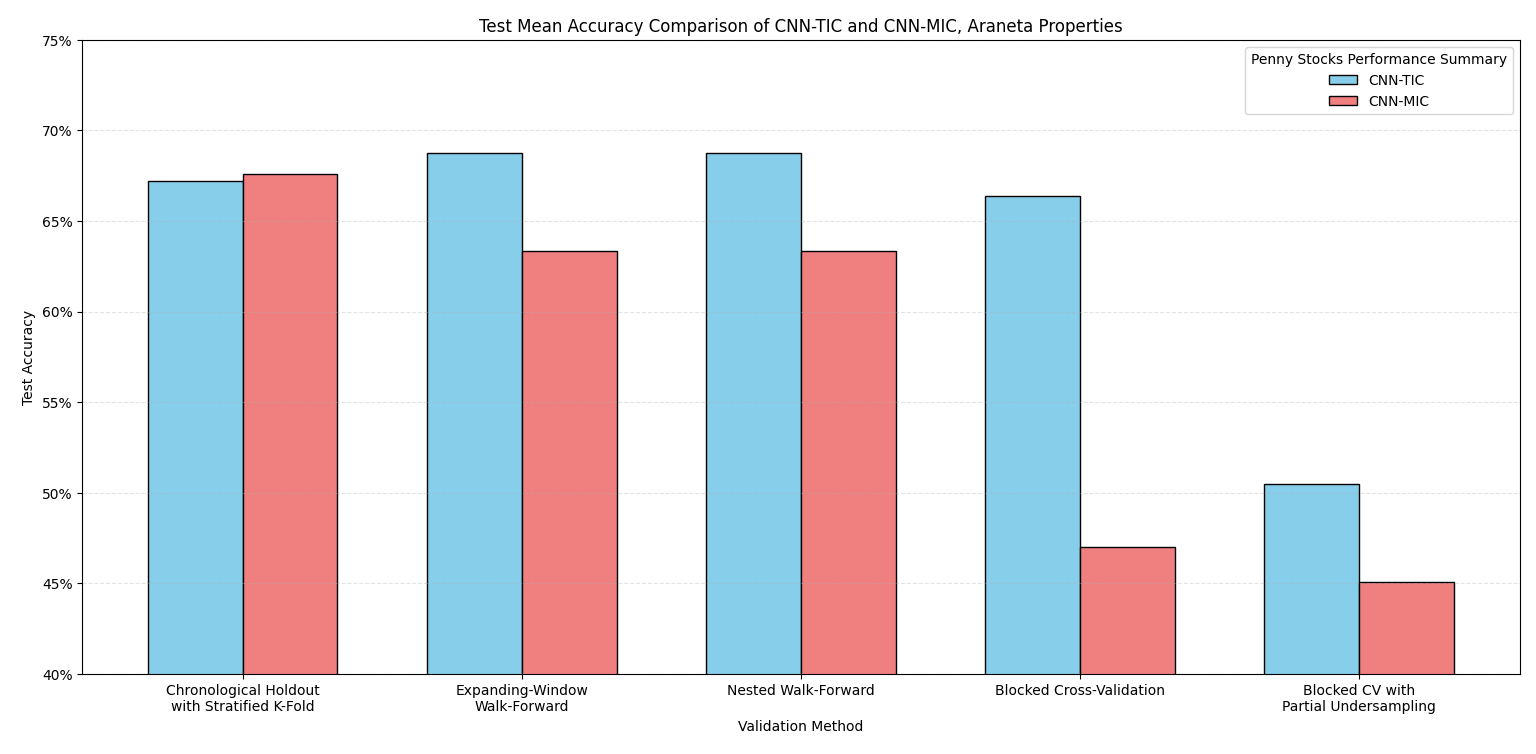
\includegraphics[width=0.8\textwidth]{../figures/ARA_TestAccuracy.png}
	
	\captionof{figure}{Test accuracy performance of CNN--TIC and CNN--MIC across selected penny stocks}
	\label{fig:test_penny_barplots}
\end{center}

\begin{center}
	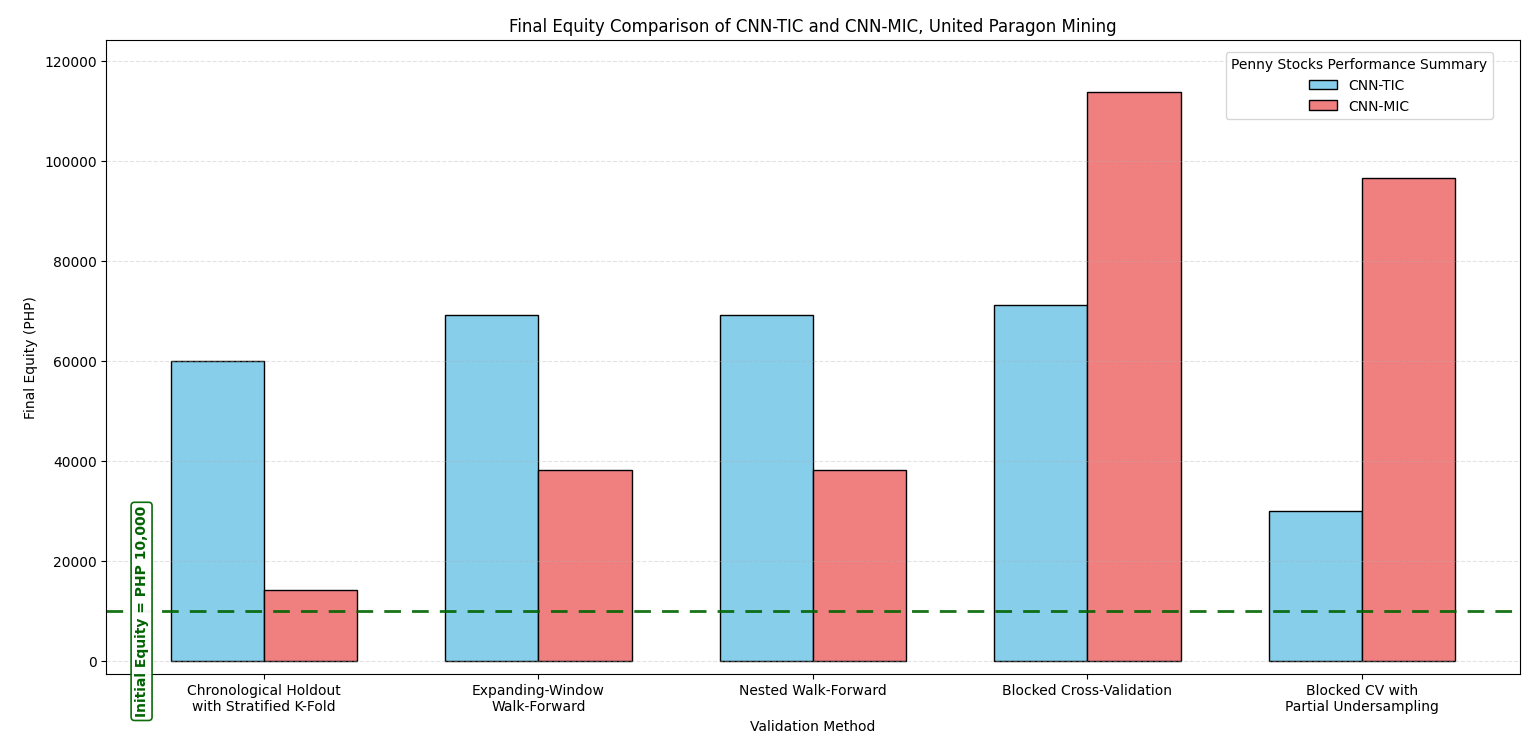
\includegraphics[width=0.8\textwidth]{../figures/UPM_FinancialAccuracy.png}
	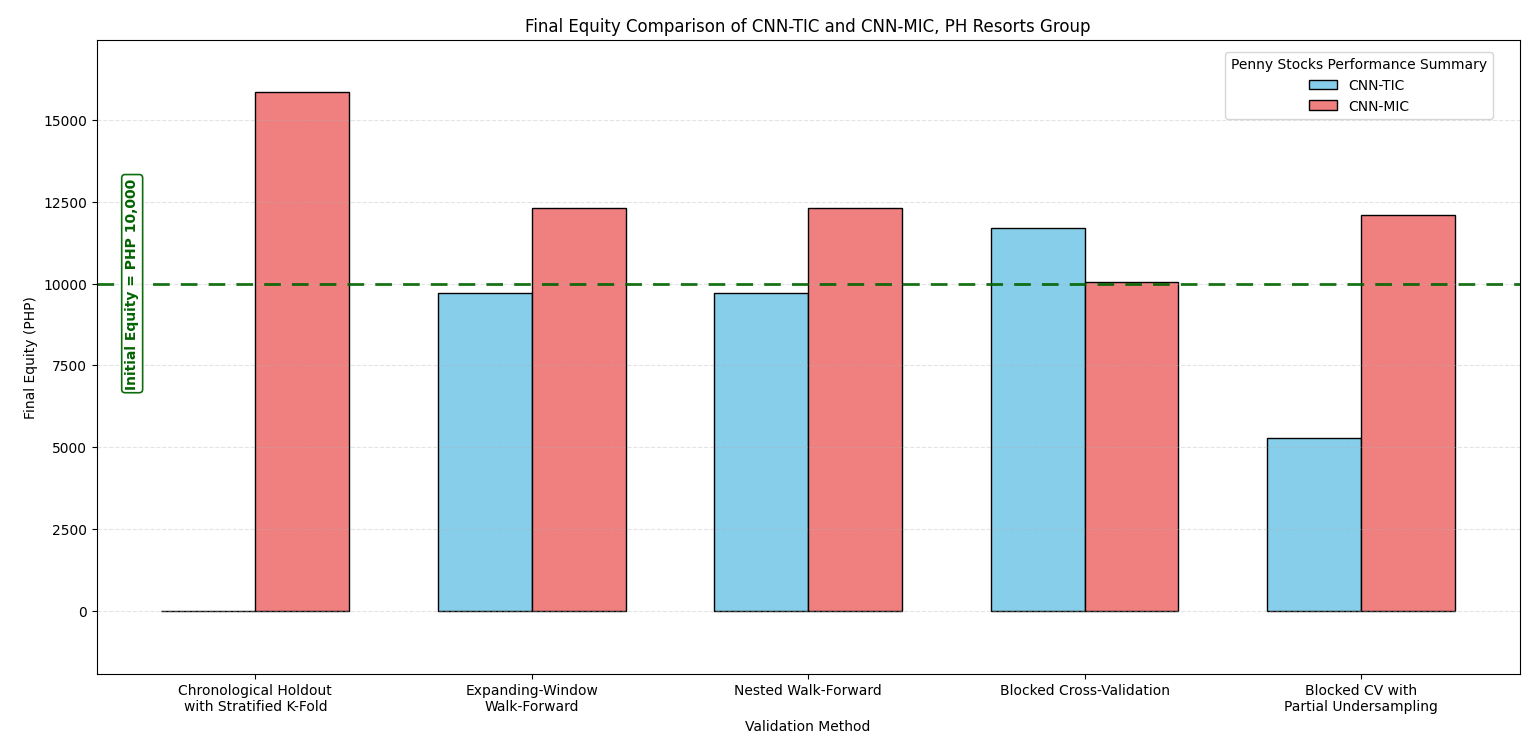
\includegraphics[width=0.8\textwidth]{../figures/PHR_FinancialAccuracy.png}
	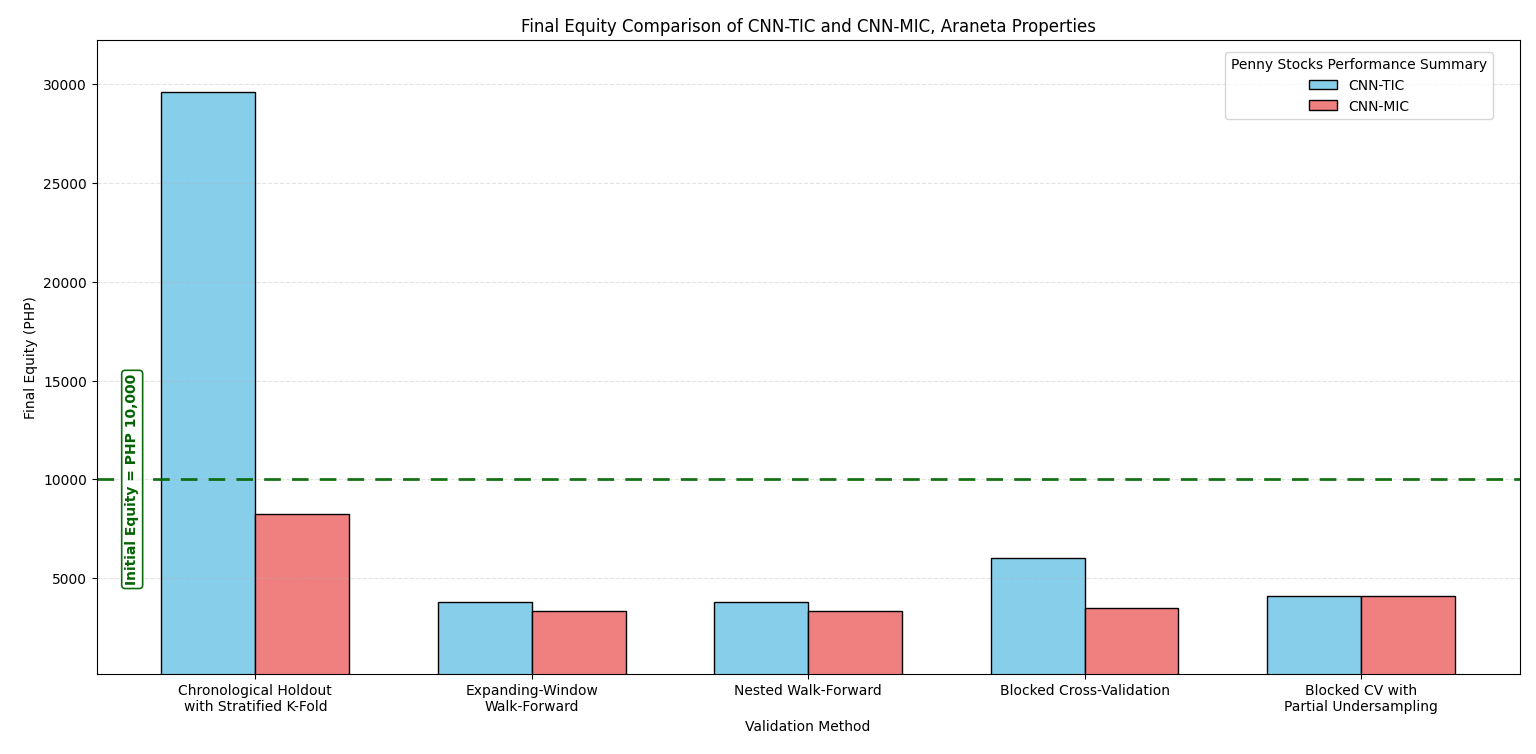
\includegraphics[width=0.8\textwidth]{../figures/ARA_FinancialAccuracy.png}
	
	\captionof{figure}{Final equity performance of CNN--TIC and CNN--MIC across selected penny stocks}
	\label{fig:fin_penny_barplots}
\end{center}

Figures~\ref{fig:test_penny_barplots} and~\ref{fig:fin_penny_barplots} show the test accuracy and final equity performance of CNN--TIC and CNN--MIC across the selected penny stocks. For this group, CNN--TIC generally remained more stable in classification, particularly for PHR and ARA. CNN--MIC showed isolated gains, such as CHV-SKF in UPM and PHR. In financial terms, however, the difference between the two models widened in some cases. CNN--MIC produced markedly higher final equity for UPM under BCV and BCV-PU and also outperformed for PHR in several settings, while CNN--TIC remained stronger for ARA. These results indicate that even when classification gains are limited, macroeconomic integration can still alter trading outcomes substantially in highly volatile equities.

\begin{center}
	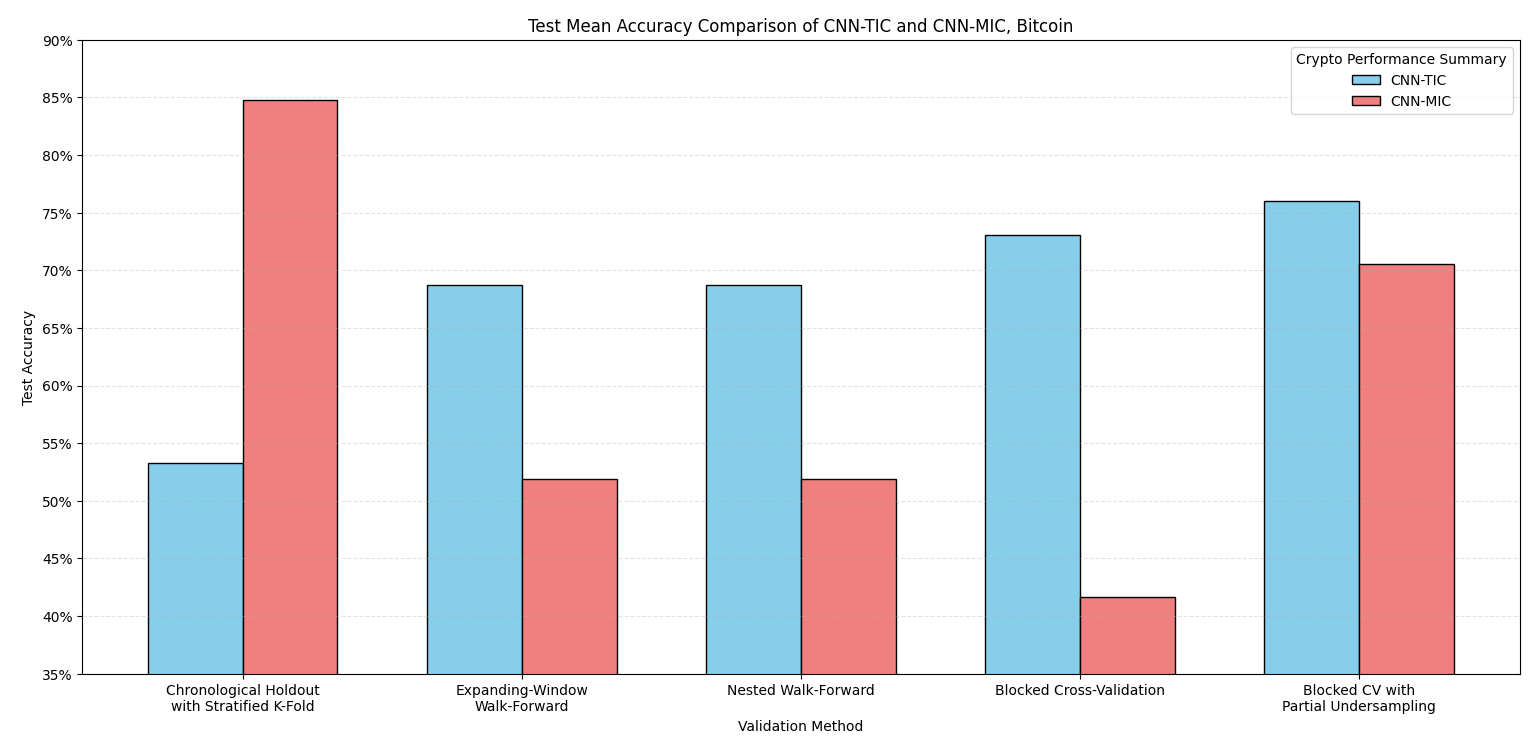
\includegraphics[width=0.8\textwidth]{../figures/BTC_TestAccuracy.png}
	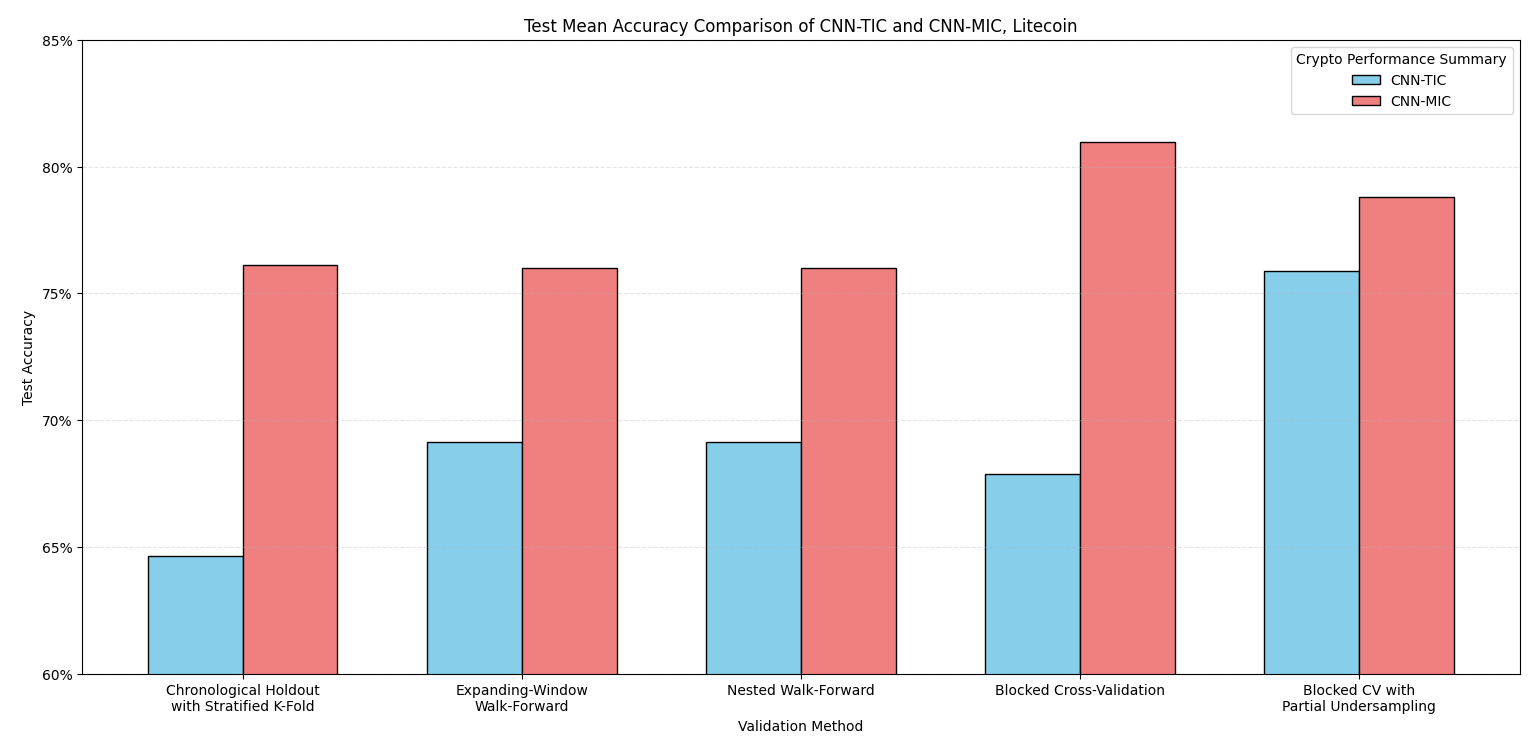
\includegraphics[width=0.8\textwidth]{../figures/LTC_TestAccuracy.png}
	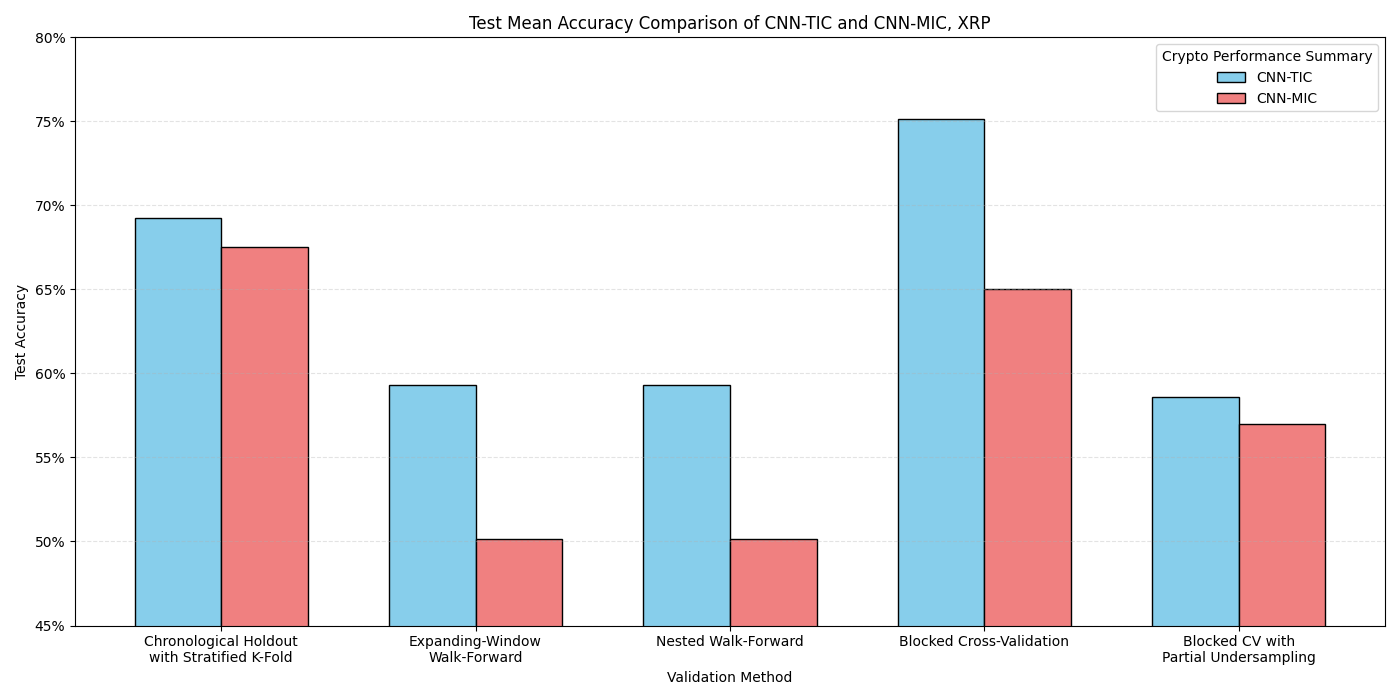
\includegraphics[width=0.8\textwidth]{../figures/XRP_TestAccuracy.png}
	
	\captionof{figure}{Test accuracy performance of CNN--TIC and CNN--MIC across selected cryptocurrency assets}
	\label{fig:test_crypto_barplots}
\end{center}

\begin{center}
	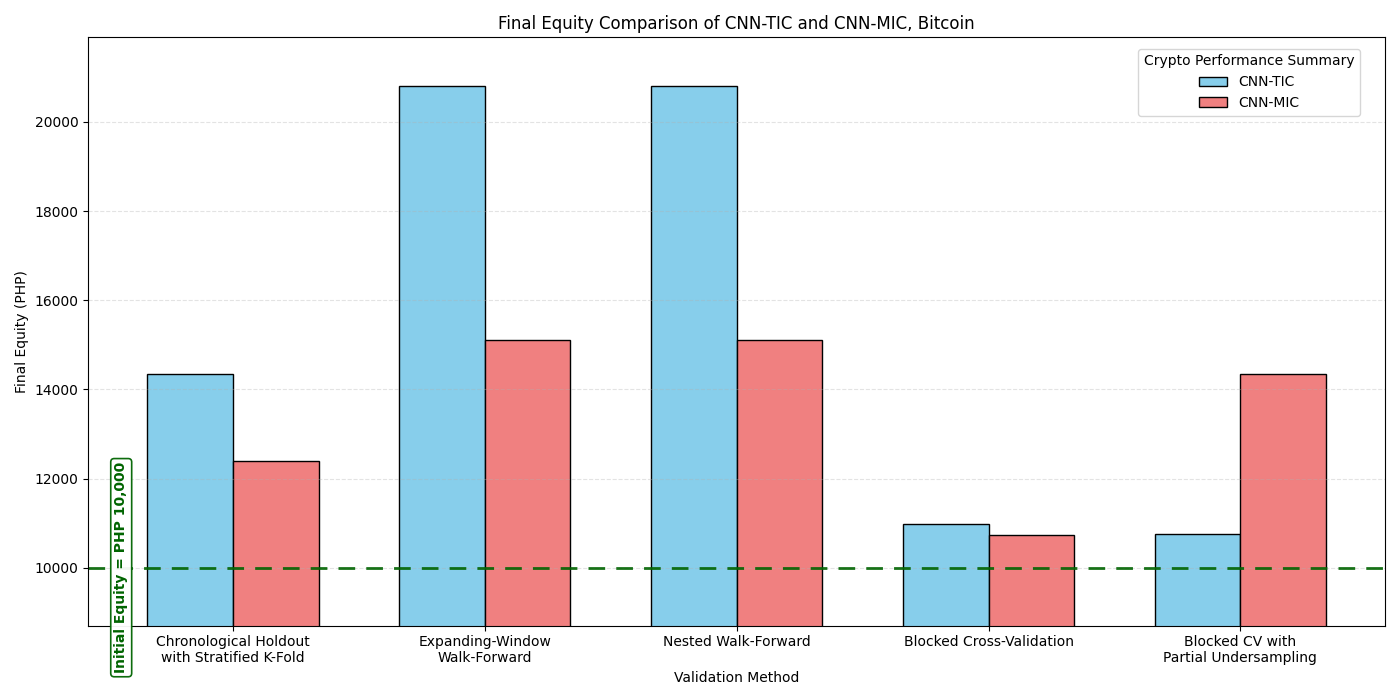
\includegraphics[width=0.8\textwidth]{../figures/BTC_FinancialAccuracy.png}
	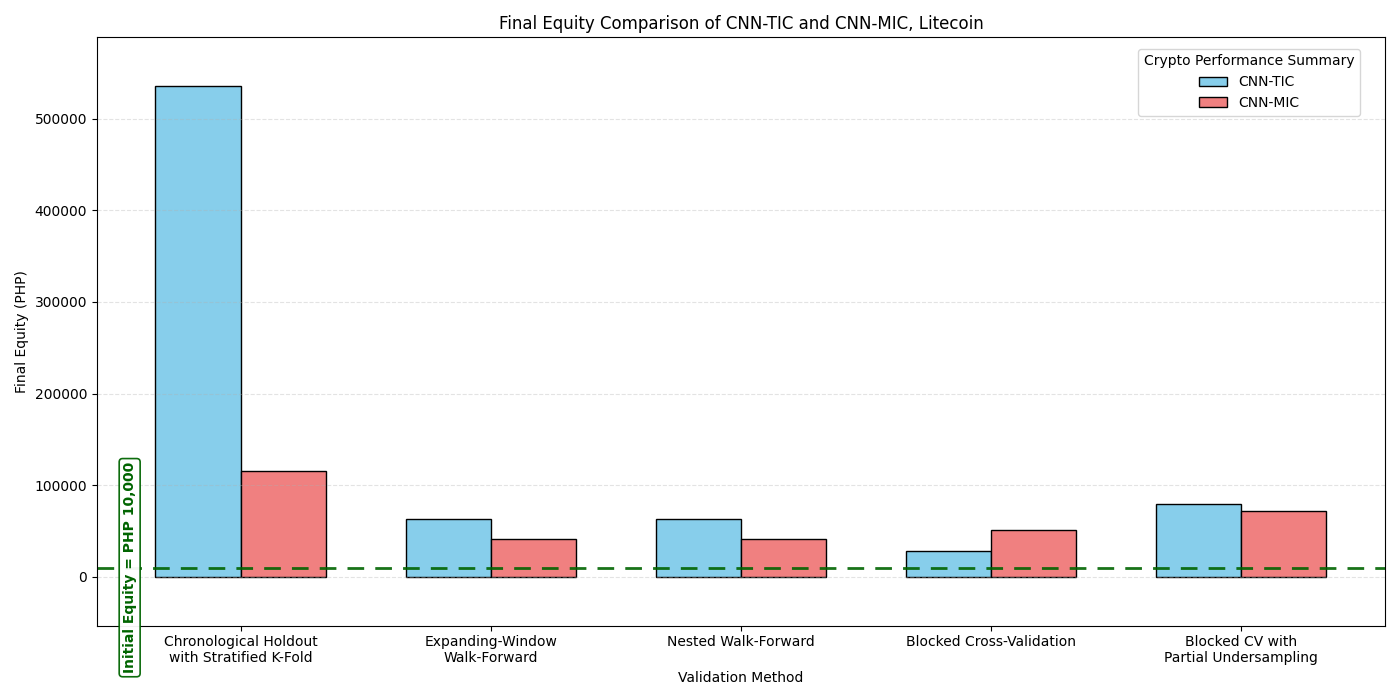
\includegraphics[width=0.8\textwidth]{../figures/LTC_FinancialAccuracy.png}
	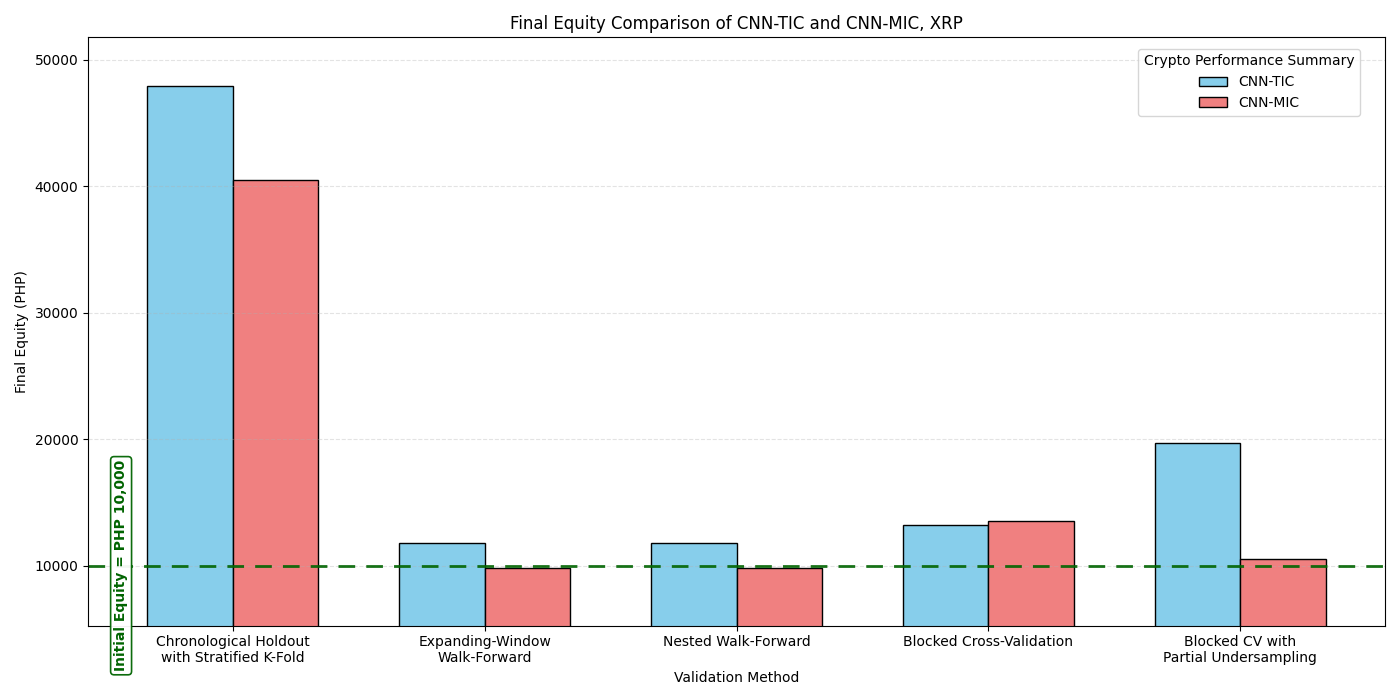
\includegraphics[width=0.8\textwidth]{../figures/XRP_FinancialAccuracy.png}
	
	\captionof{figure}{Final equity performance of CNN--TIC and CNN--MIC across selected cryptocurrency assets}
	\label{fig:fin_crypto_barplots}
\end{center}

Figures~\ref{fig:test_crypto_barplots} and~\ref{fig:fin_crypto_barplots} show the test accuracy and final equity performance of CNN--TIC and CNN--MIC across the selected cryptocurrency assets. For cryptocurrencies, the clearest classification advantage of CNN--MIC appeared in Litecoin, where it outperformed CNN--TIC across all test settings derived from the validation schemes. BTC showed a split pattern, with CNN--MIC performing strongly in CHV-SKF but lagging in several other schemes. XRP remained more favorable to CNN--TIC. The financial results were more conservative. Despite CNN--MIC's classification gains in Litecoin, CNN--TIC still achieved higher final equity in all five configurations. It also remained stronger in most BTC and XRP settings. This result shows that higher classification accuracy does not always translate directly into stronger financial performance. 
In Litecoin, CNN--MIC achieved stronger classification accuracy across the validation-derived test settings, but CNN--TIC still produced higher final equity in all five configurations. 
This means that CNN--TIC may have produced fewer correct predictions overall, but its correct signals were more financially valuable under the trading rules used in this study. 
The result supports the need to evaluate trading models using both predictive and economic metrics, since classification accuracy alone does not capture transaction timing, return magnitude, and portfolio-level outcome \cite{moosa2015directional,fischer2021feature,ozbayoglu2020deep}.

\paragraph{True-label trading performance.}

To further contextualize the financial results of CNN--TIC and CNN--MIC, the true labels were also evaluated as direct trading actions. In this evaluation, the saved Buy, Hold, and Sell labels of each asset were used as the input trading signals. The same financial evaluation procedure was applied, including the initial balance, commission, take-profit, stop-loss, yearly return computation, and final equity calculation used for the CNN-based models.

This evaluation shows the financial performance that can be obtained when the generated labels are used directly as trading signals. The results provide a reference point for comparing the financial outcomes of CNN--TIC and CNN--MIC, since both models attempt to predict the same Buy, Hold, and Sell actions.

The table below presents the financial performance obtained when the true labels were used as trading signals. Among the blue-chip stocks, SMI produced the highest final equity with PHP~71,287.24, while AC and JFC reached PHP~48,134.44 and PHP~39,998.07, respectively. The cryptocurrency assets produced the largest final equities, with LTC reaching PHP~423,881.11, XRP reaching PHP~315,861.28, and BTC reaching PHP~296,652.86. Among the penny stocks, UPM obtained the highest final equity at PHP~77,362.25, followed by ARA and PHR.

\begin{table}[H]
	\centering
	\caption{Financial performance using true labels as trading actions}
	\resizebox{\textwidth}{!}{
		\begin{tabular}{llrrr}
			\toprule
			Asset & Category & Final Equity & Mean Annual Return & Std. Annual Return \\
			\midrule
			AC  & Blue-chip Stocks & 48,134.44  & 121.03\% & 37.96\% \\
			JFC & Blue-chip Stocks & 39,998.07  & 102.31\% & 39.87\% \\
			SMI & Blue-chip Stocks & 71,287.24  & 172.90\% & 79.23\% \\
			ARA & Penny Stocks     & 68,571.52  & 168.64\% & 80.65\% \\
			PHR & Penny Stocks     & 67,070.60  & 163.55\% & 69.10\% \\
			UPM & Penny Stocks     & 77,362.25  & 179.34\% & 36.53\% \\
			BTC & Cryptocurrency   & 296,652.86 & 450.30\% & 110.72\% \\
			LTC & Cryptocurrency   & 423,881.11 & 541.45\% & 21.41\% \\
			XRP & Cryptocurrency   & 315,861.28 & 464.15\% & 140.53\% \\
			\bottomrule
		\end{tabular}
	}
\end{table}

The true-label results are substantially higher than the CNN--TIC and CNN--MIC financial results reported in Appendix~\ref{app:experiment2_tables}. This gap is expected because the true labels are generated from the actual turning points of the price series, while CNN--TIC and CNN--MIC only estimate those labels from technical and macroeconomic image representations. The comparison therefore shows that the labeling method itself can produce strong financial outcomes when used directly, but the CNN models still lose performance when approximating those actions from input features. This supports the need to evaluate the models not only by classification accuracy, but also by how closely their predicted trading actions approach the financial behavior of the true-label reference.

\paragraph{Volatile-period evaluation from 2021 to 2022.}

To further examine the relationship between classification accuracy and profitability, an additional volatile-period evaluation was conducted using 2021 to 2022 as the evaluation window. This period was selected to represent a more unstable market condition following the pandemic-driven disruption in financial markets. The evaluation followed the Chronological Holdout Validation with Stratified K-Fold (CHV-SKF) setup. In this setup, the models were trained using data up to 2020 and evaluated on the period after 2020. 

The volatile-period evaluation used only the prediction rows dated from 2021-01-01 to 2022-12-31. For PSE assets, the first available trading date was 2021-01-04. For cryptocurrency assets, the first available date was 2021-01-01. Classification accuracy and macro F1 were computed from the saved prediction files. Financial performance was computed using the corresponding backtest outputs under the same take-profit, stop-loss, and commission rules used in Algorithm~2.

Table~\ref{tab:volatile-period-performance} summarizes the model performance during the 2021--2022 volatile period. The results show that higher accuracy did not always correspond to higher final equity. CNN--MIC produced higher accuracy in JFC, SMI, PHR, UPM, BTC, LTC, and XRP. However, the higher-accuracy model was not always the more profitable model. For SMI, UPM, BTC, and LTC, CNN--MIC achieved higher classification accuracy, but CNN--TIC produced higher final equity. For AC, the opposite pattern appeared, where CNN--TIC achieved higher accuracy, but CNN--MIC produced higher final equity.

\begin{table}[H]
	\centering
	\caption{Volatile-period performance of CNN--TIC and CNN--MIC using 2021--2022 as evaluation window}
	\label{tab:volatile-period-performance}
	\resizebox{\textwidth}{!}{
		\begin{tabular}{lrrrrrr}
			\toprule
			Asset & TIC Accuracy & MIC Accuracy & TIC Final Equity & MIC Final Equity \\
			\midrule
			AC  & 71.66\% & 61.54\% & 11,993.69 & 14,818.66 \\
			JFC & 65.59\% & 70.85\% & 9,075.38  & 9,251.30  \\
			SMI & 75.10\% & 75.91\% & 18,992.57 & 16,250.71 \\
			ARA & 73.50\% & 73.04\% & 25,221.47 & 15,491.72 \\
			PHR & 58.30\% & 61.94\% & 6,955.87  & 10,722.70 \\
			UPM & 67.49\% & 72.70\% & 11,968.99 & 8,914.22  \\
			BTC & 69.59\% & 83.01\% & 12,660.80 & 12,403.82 \\
			LTC & 62.33\% & 72.60\% & 59,063.82 & 58,106.17 \\
			XRP & 70.41\% & 74.25\% & 36,131.72 & 36,957.03 \\
			\bottomrule
			\end{tabular}
		}
	\end{table}

These results strengthen the main finding of Experiment~2. During the 2021--2022 volatile period, CNN--MIC had the higher accuracy in seven of the nine assets. However, CNN--MIC had the higher final equity in only four assets. This shows that accuracy and profitability can diverge more clearly during unstable market conditions. A model may correctly classify more days overall, but its profitable signals may occur at weaker entry or exit points. 
Likewise, a model with lower accuracy may still produce higher equity if its correct Buy and Sell signals occur near larger price movements. Thus, the volatile-period evaluation supports the use of both predictive metrics and financial metrics when assessing CNN-based trading models.

\subsection{Experiment 3: SHAP-Based Interpretation of CNN--MIC Across Validation Schemes}

 The analysis was applied to the predicted-class outputs of the model and was restricted to correctly predicted test samples in order to focus on feature contributions associated with valid model decisions. This experiment was intended to complement the numerical findings of Experiments 1 and 2 by showing how the model combined technical and macroeconomic information under different evaluation settings.

Across the analyzed SHAP results, technical indicators generally remained the dominant source of information in CNN--MIC. However, macroeconomic variables still showed visible contributions, and their relative importance varied depending on the validation scheme. This indicates that the inclusion of macroeconomic indicators did not replace the technical representation of the model. Instead, it enriched the input space by providing additional context that became more or less useful depending on the evaluation setting.

Figure~\ref{fig:shap_ac_bcvpu_rows} shows the predicted-class SHAP row importance for Ayala Corporation under BCV-PU, which is used here as a representative example. In this scheme, Williams \%R appeared as the most influential technical contributor, followed by CMO and CCI. Among the macroeconomic variables, Reverse Repurchase Rate (RRP) and Purchasing Power of Peso (PPP) showed the strongest contributions, while Oil, Gold, and Inflation Rate had smaller but still visible influence. The figure shows that although macroeconomic variables were meaningfully involved in the prediction process, the dominant contributions still came from technical rows.

\begin{figure}[H]
	\centering
	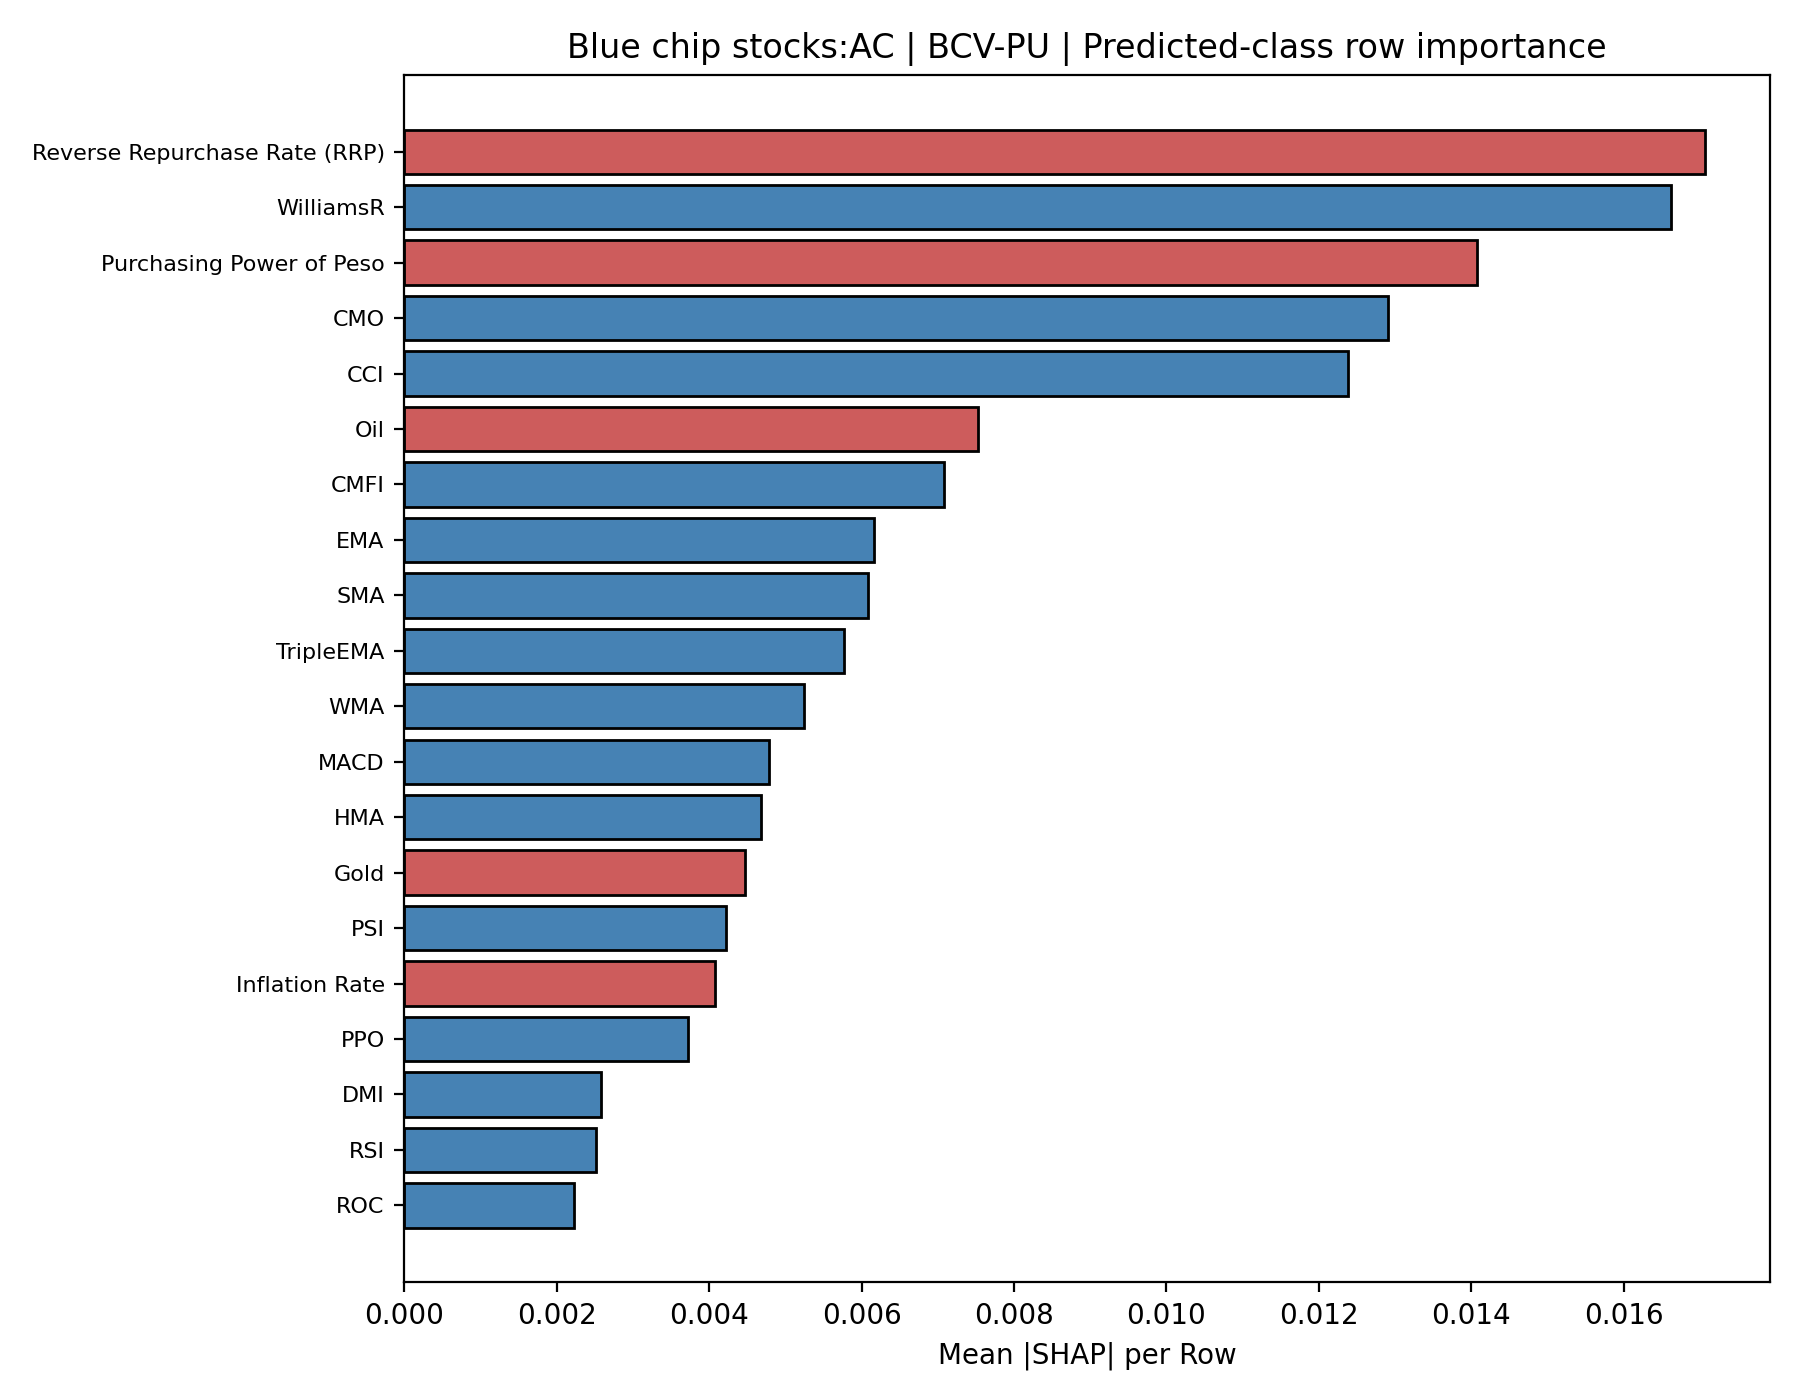
\includegraphics[width=1\textwidth]{../figures/AC_PredictedClassRowImportance.png}
	\caption{Predicted-class SHAP row importance for Ayala Corporation under BCV-PU. }
	\label{fig:shap_ac_bcvpu_rows}
\end{figure}

The remaining validation schemes followed the same general pattern, where technical indicators accounted for the larger share of feature contribution and macroeconomic variables acted as supplementary inputs. What changed across schemes was not the overall dominance of technical information, but the relative strength of the macroeconomic variables and the ranking of the most influential rows. This suggests that the contribution of macroeconomic information in CNN--MIC is sensitive to the structure of the evaluation procedure. In the case of AC, these variables functioned as supporting contextual signals rather than as the primary basis of prediction, which reinforces the broader result of this chapter that macroeconomic integration is condition-dependent and works best as a complement to technical information rather than as a replacement for it. The predicted-class SHAP row importance plots for the remaining assets are presented in Appendix~\ref{app:experiment3_shap}.



 %results and discussion
\chapter{Conclusions and Recommendations}

This study developed and evaluated two CNN-based image representations for financial trend prediction, namely the baseline CNN--TIC model and the proposed CNN--MIC model. CNN--TIC used technical indicators only, while CNN--MIC extended the image representation by integrating macroeconomic indicators with technical indicators. Both models were evaluated under the same preprocessing pipeline, labeling strategy, validation procedures, and trading simulation rules across selected blue-chip stocks and penny stocks from the PSE market, as well as selected cryptocurrency assets.

The results showed that the inclusion of macroeconomic indicators can improve prediction performance in selected cases, but the advantage was not consistent across all assets and validation settings. CNN--MIC produced higher results in some stocks and cryptocurrencies, which suggests that macroeconomic indicators can contribute in terms of financial trend prediction. However, CNN--TIC remained more stable in many cases, such as when the technical structure of the asset appeared sufficient for prediction.The financial evaluation also showed that stronger classification results did not always lead to better trading returns. This indicates that predictive accuracy alone is not enough to produce stronger financial performance.

Overall, the study shows that adding macroeconomic indicators is a viable extension of the CNN--TIC framework, even if it was not consistent across all assets and evaluation settings. The main contribution of this work is the demonstration that macroeconomic indicators can be incorporated into an image-based CNN trading representation and may provide measurable benefits under specific market conditions.

Future work should address the dataset limitations by testing more assets, longer time frame for historical data, and adding more macroeconomic indicators that may contribute to its performance. Other image-based strategies and CNN architectures may also be explored to better capture the interaction between technical and macroeconomic signals. Lastly, future work may further analyze the model’s behavior when macroeconomic indicators are contributing most in improving prediction performance. %conclusions and recommendations
\appendix
\chapter{Appendix}

\section{Dataset}

\begin{center}
	\scriptsize
	\captionof{table}{Number of dataset rows per asset}
	\label{tab:appendix_dataset_rows}
	\vspace{0.5em}
	\resizebox{1\textwidth}{!}{%
		{\renewcommand{\arraystretch}{1.2}
			\begin{tabular}{llr}
				\hline
				Category & Asset & Dataset Rows \\
				\hline
				Blue-chip Stocks & Ayala Corporation & 3,235 \\
				Blue-chip Stocks & Jollibee Foods Corporation & 3,234 \\
				Blue-chip Stocks & SM Investments Corporation & 3,233 \\
				\hline
				Penny Stocks & Araneta Properties & 2,956 \\
				Penny Stocks & PH Resorts Group & 2,680 \\
				Penny Stocks & United Paragon Mining Corporation & 2,240 \\
				\hline
				Cryptocurrency & Bitcoin & 4,848 \\
				Cryptocurrency & Litecoin & 3,283 \\
				Cryptocurrency & XRP & 3,627 \\
	
				\hline
			\end{tabular}
		}
	}
\end{center}
Table~\ref{tab:appendix_dataset_rows} shows the number of dataset rows for each asset included in the study. The dataset sizes are not the same across all assets. Bitcoin has the largest dataset, while United Paragon Mining Corporation has the smallest.


\section{Experiment 1 Tables}
\label{app:experiment1_tables}


\begin{center}
	\scriptsize
	\captionof{table}{Validation performance of blue-chip stocks}
	\label{tab:val_bluechip}
	\vspace{0.5em}
	\resizebox{\textwidth}{!}{%
		{\renewcommand{\arraystretch}{1.3}
			\begin{tabular}{lllccccc}
				\hline
				Stock & Model & Metric & CHV-SKF & EW-WFV & NWFV & BCV & BCV-PU \\
				\hline
				Ayala Corporation & CNN--TIC & Accuracy & 68.19\% & 71.79\% & 73.32\% & 67.87\% & 70.07\% \\
				& CNN--TIC & Macro F1 & 51.56\% & 58.49\% & 58.31\% & 52.65\% & 52.39\% \\
				& CNN--MIC & Accuracy & 65.33\% & 72.08\% & 71.72\% & 66.80\% & 66.91\% \\
				& CNN--MIC & Macro F1 & 49.69\% & 57.22\% & 57.02\% & 51.51\% & 49.55\% \\
				\hline
				Jollibee Food Corporation & CNN--TIC & Accuracy & 67.86\% & 64.86\% & 66.28\% & 60.56\% & 69.50\% \\
				& CNN--TIC & Macro F1 & 51.69\% & 49.57\% & 50.91\% & 45.88\% & 47.49\% \\
				& CNN--MIC & Accuracy & 67.29\% & 69.39\% & 68.16\% & 64.07\% & 68.26\% \\
				& CNN--MIC & Macro F1 & 51.38\% & 51.28\% & 52.72\% & 46.46\% & 46.73\% \\
				\hline
				SM Investments & CNN--TIC & Accuracy & 72.85\% & 75.40\% & 76.91\% & 70.52\% & 78.89\% \\
				& CNN--TIC & Macro F1 & 55.31\% & 63.52\% & 63.74\% & 56.60\% & 59.55\% \\
				& CNN--MIC & Accuracy & 73.66\% & 74.03\% & 75.92\% & 72.05\% & 74.68\% \\
				& CNN--MIC & Macro F1 & 55.94\% & 61.65\% & 63.27\% & 56.92\% & 57.69\% \\
				\hline
			\end{tabular}
	}}
\end{center}

\begin{center}
	\scriptsize
	\captionof{table}{Validation performance of penny stocks}
	\label{tab:val_penny}
	\vspace{0.5em}
	\resizebox{\textwidth}{!}{%
		{\renewcommand{\arraystretch}{1.3}
			\begin{tabular}{lllccccc}
				\hline
				Stock & Model & Metric & CHV-SKF & EW-WFV & NWFV & BCV & BCV-PU \\
				\hline
				United Paragon Mining & CNN--TIC & Accuracy & 67.17\% & 70.37\% & 73.04\% & 67.50\% & 66.77\% \\
				& CNN--TIC & Macro F1 & 54.35\% & 56.38\% & 58.03\% & 52.14\% & 50.75\% \\
				& CNN--MIC & Accuracy & 62.60\% & 69.21\% & 71.11\% & 67.30\% & 68.91\% \\
				& CNN--MIC & Macro F1 & 50.97\% & 55.98\% & 57.25\% & 50.66\% & 50.36\% \\
				\hline
				PH Resorts Group & CNN--TIC & Accuracy & 73.11\% & 70.53\% & 75.00\% & 68.58\% & 69.97\% \\
				& CNN--TIC & Macro F1 & 52.41\% & 56.45\% & 57.83\% & 49.35\% & 45.48\% \\
				& CNN--MIC & Accuracy & 70.84\% & 69.55\% & 71.39\% & 66.89\% & 63.79\% \\
				& CNN--MIC & Macro F1 & 50.36\% & 56.80\% & 57.21\% & 48.84\% & 46.35\% \\
				\hline
				Araneta Properties & CNN--TIC & Accuracy & 70.20\% & 72.90\% & 72.80\% & 73.60\% & 72.94\% \\
				& CNN--TIC & Macro F1 & 51.92\% & 61.92\% & 62.37\% & 58.45\% & 57.75\% \\
				& CNN--MIC & Accuracy & 70.09\% & 72.75\% & 70.83\% & 73.06\% & 73.84\% \\
				& CNN--MIC & Macro F1 & 52.12\% & 64.02\% & 60.66\% & 57.61\% & 56.74\% \\
				\hline
			\end{tabular}
	}}
\end{center}

\begin{center}
	\scriptsize
	\captionof{table}{Validation performance of cryptocurrencies}
	\label{tab:val_crypto}
	\vspace{0.5em}
	\resizebox{\textwidth}{!}{%
		{\renewcommand{\arraystretch}{1.3}
			\begin{tabular}{lllccccc}
				\hline
				Stock & Model & Metric & CHV-SKF & EW-WFV & NWFV & BCV & BCV-PU \\
				\hline
				Bitcoin & CNN--TIC & Accuracy & 67.71\% & 66.33\% & 67.81\% & 69.47\% & 67.59\% \\
				& CNN--TIC & Macro F1 & 48.83\% & 53.64\% & 55.16\% & 48.01\% & 47.58\% \\
				& CNN--MIC & Accuracy & 66.79\% & 67.26\% & 67.92\% & 66.88\% & 68.42\% \\
				& CNN--MIC & Macro F1 & 47.61\% & 55.04\% & 54.76\% & 47.09\% & 48.61\% \\
				\hline
				Litecoin & CNN--TIC & Accuracy & 70.27\% & 68.89\% & 71.87\% & 69.44\% & 66.09\% \\
				& CNN--TIC & Macro F1 & 54.85\% & 54.85\% & 55.11\% & 51.50\% & 48.34\% \\
				& CNN--MIC & Accuracy & 72.53\% & 72.73\% & 72.95\% & 66.81\% & 63.37\% \\
				& CNN--MIC & Macro F1 & 54.98\% & 56.61\% & 55.77\% & 49.62\% & 45.98\% \\
				\hline
				XRP & CNN--TIC & Accuracy & 73.04\% & 73.33\% & 73.96\% & 70.41\% & 67.95\% \\
				& CNN--TIC & Macro F1 & 54.82\% & 56.11\% & 57.67\% & 52.68\% & 50.81\% \\
				& CNN--MIC & Accuracy & 72.83\% & 70.49\% & 71.41\% & 70.89\% & 63.89\% \\
				& CNN--MIC & Macro F1 & 53.65\% & 54.98\% & 55.91\% & 52.43\% & 47.64\% \\
				\hline
			\end{tabular}
	}}
\end{center}

\section{Experiment 2 Tables}
\label{app:experiment2_tables}
\begin{center}
	\scriptsize
	\captionof{table}{Test classification performance of blue-chip stocks}
	\label{tab:test_bluechip}
	\vspace{0.5em}
	\resizebox{\textwidth}{!}{%
		{\renewcommand{\arraystretch}{1.3}
			\begin{tabular}{lllccccc}
				\hline
				Stock & Model & Metric & CHV-SKF & EW-WFV & NWFV & BCV & BCV-PU \\
				\hline
				Ayala Corporation & CNN--TIC & Accuracy & 69.24\% & 67.55\% & 67.55\% & 74.22\% & 65.84\% \\
				& CNN--TIC & Macro F1 & 52.43\% & 51.36\% & 51.36\% & 51.24\% & 49.72\% \\
				& CNN--MIC & Accuracy & 64.76\% & 63.04\% & 63.04\% & 65.68\% & 68.63\% \\
				& CNN--MIC & Macro F1 & 49.26\% & 49.02\% & 49.02\% & 50.51\% & 52.36\% \\
				\hline
				Jollibee Food Corp. & CNN--TIC & Accuracy & 67.02\% & 68.90\% & 68.90\% & 78.38\% & 70.30\% \\
				& CNN--TIC & Macro F1 & 51.66\% & 54.37\% & 54.37\% & 52.85\% & 52.77\% \\
				& CNN--MIC & Accuracy & 68.34\% & 69.05\% & 69.05\% & 73.09\% & 72.78\% \\
				& CNN--MIC & Macro F1 & 48.41\% & 53.07\% & 53.07\% & 56.27\% & 51.74\% \\
				\hline
				SM Investments & CNN--TIC & Accuracy & 70.98\% & 64.54\% & 64.54\% & 70.14\% & 83.51\% \\
				& CNN--TIC & Macro F1 & 54.28\% & 49.09\% & 49.09\% & 50.99\% & 55.35\% \\
				& CNN--MIC & Accuracy & 69.39\% & 46.81\% & 46.81\% & 65.79\% & 79.00\% \\
				& CNN--MIC & Macro F1 & 51.36\% & 39.54\% & 39.54\% & 49.82\% & 57.03\% \\
				\hline
			\end{tabular}
	}}
\end{center}

\begin{center}
	\scriptsize
	\captionof{table}{Test classification performance of penny stocks}
	\label{tab:test_penny}
	\vspace{0.5em}
	\resizebox{\textwidth}{!}{%
		{\renewcommand{\arraystretch}{1.3}
			\begin{tabular}{lllccccc}
				\hline
				Stock & Model & Metric & CHV-SKF & EW-WFV & NWFV & BCV & BCV-PU \\
				\hline
				United Paragon Mining & CNN--TIC & Accuracy & 69.21\% & 68.52\% & 68.52\% & 70.82\% & 69.18\% \\
				& CNN--TIC & Macro F1 & 53.67\% & 57.74\% & 57.74\% & 59.58\% & 55.69\% \\
				& CNN--MIC & Accuracy & 73.73\% & 66.89\% & 66.89\% & 69.51\% & 56.72\% \\
				& CNN--MIC & Macro F1 & 51.11\% & 54.20\% & 54.20\% & 59.49\% & 50.54\% \\
				\hline
				PH Resorts Group & CNN--TIC & Accuracy & 59.37\% & 70.76\% & 70.76\% & 75.89\% & 75.27\% \\
				& CNN--TIC & Macro F1 & 46.99\% & 50.72\% & 50.72\% & 51.35\% & 35.99\% \\
				& CNN--MIC & Accuracy & 65.88\% & 70.92\% & 70.92\% & 35.77\% & 40.90\% \\
				& CNN--MIC & Macro F1 & 47.84\% & 54.04\% & 54.04\% & 25.57\% & 28.47\% \\
				\hline
				Araneta Properties & CNN--TIC & Accuracy & 67.20\% & 68.73\% & 68.73\% & 66.35\% & 50.48\% \\
				& CNN--TIC & Macro F1 & 50.85\% & 49.61\% & 49.61\% & 48.38\% & 40.69\% \\
				& CNN--MIC & Accuracy & 67.58\% & 63.33\% & 63.33\% & 46.98\% & 45.08\% \\
				& CNN--MIC & Macro F1 & 50.61\% & 49.41\% & 49.41\% & 39.96\% & 36.49\% \\
				\hline
			\end{tabular}
	}}
\end{center}

\begin{center}
	\scriptsize
	\captionof{table}{Test classification performance of cryptocurrencies}
	\label{tab:test_crypto}
	\vspace{0.5em}
	\resizebox{\textwidth}{!}{%
		{\renewcommand{\arraystretch}{1.3}
			\begin{tabular}{lllccccc}
				\hline
				Stock & Model & Metric & CHV-SKF & EW-WFV & NWFV & BCV & BCV-PU \\
				\hline
				Bitcoin & CNN--TIC & Accuracy & 53.25\% & 68.71\% & 68.71\% & 73.08\% & 75.99\% \\
				& CNN--TIC & Macro F1 & 32.94\% & 48.12\% & 48.12\% & 40.16\% & 39.19\% \\
				& CNN--MIC & Accuracy & 84.75\% & 51.87\% & 51.87\% & 41.68\% & 70.58\% \\
				& CNN--MIC & Macro F1 & 37.47\% & 39.89\% & 39.89\% & 27.77\% & 40.49\% \\
				\hline
				Litecoin & CNN--TIC & Accuracy & 64.66\% & 69.13\% & 69.13\% & 67.88\% & 75.88\% \\
				& CNN--TIC & Macro F1 & 49.69\% & 53.45\% & 53.45\% & 48.24\% & 54.84\% \\
				& CNN--MIC & Accuracy & 76.12\% & 75.99\% & 75.99\% & 80.98\% & 78.79\% \\
				& CNN--MIC & Macro F1 & 51.15\% & 54.31\% & 54.31\% & 52.71\% & 53.83\% \\
				\hline
				XRP & CNN--TIC & Accuracy & 69.25\% & 59.31\% & 59.31\% & 75.13\% & 58.58\% \\
				& CNN--TIC & Macro F1 & 47.90\% & 42.79\% & 42.79\% & 47.43\% & 44.40\% \\
				& CNN--MIC & Accuracy & 67.53\% & 50.16\% & 50.16\% & 65.04\% & 57.02\% \\
				& CNN--MIC & Macro F1 & 44.58\% & 31.80\% & 31.80\% & 45.47\% & 36.28\% \\
				\hline
			\end{tabular}
	}}
\end{center}

\begin{center}
	\scriptsize
	\captionof{table}{Financial performance of blue-chip stocks}
	\label{tab:fin_bluechip}
	\vspace{0.5em}
	\resizebox{\textwidth}{!}{%
		{\renewcommand{\arraystretch}{1.3}
			\begin{tabular}{lllccccc}
				\hline
				Stock & Model & Metric & CHV-SKF & EW-WFV & NWFV & BCV & BCV-PU \\
				\hline
				Ayala Corporation & CNN--TIC & Final Equity & 17,384.65 & 9,233.18 & 9,233.18 & 15,851.34 & 11,100.64 \\
				& CNN--TIC & Mean Return & 11.32\% & -3.21\% & -3.21\% & 16.06\% & 2.22\% \\
				& CNN--TIC & Std Return & 12.78\% & 13.64\% & 13.64\% & 18.95\% & 7.93\% \\
				& CNN--MIC & Final Equity & 21,715.91 & 12,314.28 & 12,314.28 & 9,853.95 & 13,770.70 \\
				& CNN--MIC & Mean Return & 16.55\% & 6.24\% & 6.24\% & -1.17\% & 10.78\% \\
				& CNN--MIC & Std Return & 15.37\% & 11.57\% & 11.57\% & 13.12\% & 19.82\% \\
				\hline
				Jollibee Food Corporation & CNN--TIC & Final Equity & 12,194.60 & 11,734.50 & 11,734.50 & 11,443.29 & 10,258.05 \\
				& CNN--TIC & Mean Return & 4.18\% & 6.27\% & 6.27\% & 5.30\% & 1.19\% \\
				& CNN--TIC & Std Return & 12.00\% & 15.70\% & 15.70\% & 14.59\% & 10.25\% \\
				& CNN--MIC & Final Equity & 11,750.14 & 15,167.17 & 15,167.17 & 12,025.72 & 10,577.82 \\
				& CNN--MIC & Mean Return & 3.34\% & 15.31\% & 15.31\% & 6.64\% & 3.66\% \\
				& CNN--MIC & Std Return & 11.54\% & 12.05\% & 12.05\% & 9.72\% & 23.78\% \\
				\hline
				SM Investments & CNN--TIC & Final Equity & 31,374.99 & 10,958.34 & 10,958.34 & 12,047.73 & 12,832.53 \\
				& CNN--TIC & Mean Return & 26.68\% & 3.28\% & 3.28\% & 6.60\% & 8.90\% \\
				& CNN--TIC & Std Return & 16.06\% & 8.64\% & 8.64\% & 9.43\% & 12.50\% \\
				& CNN--MIC & Final Equity & 25,299.63 & 8,768.61 & 8,768.61 & 9,058.43 & 13,229.06 \\
				& CNN--MIC & Mean Return & 21.14\% & -4.14\% & -4.14\% & -2.93\% & 9.61\% \\
				& CNN--MIC & Std Return & 17.79\% & 6.94\% & 6.94\% & 10.21\% & 4.83\% \\
				\hline
			\end{tabular}
	}}
\end{center}

\begin{center}
	\scriptsize
	\captionof{table}{Financial performance of penny stocks}
	\label{tab:fin_penny}
	\vspace{0.5em}
	\resizebox{\textwidth}{!}{%
		{\renewcommand{\arraystretch}{1.3}
			\begin{tabular}{lllccccc}
				\hline
				Stock & Model & Metric & CHV-SKF & EW-WFV & NWFV & BCV & BCV-PU \\
				\hline
				United Paragon Mining & CNN--TIC & Final Equity & 60,090.92 & 69,285.79 & 69,285.79 & 71,290.94 & 30,109.73 \\
				& CNN--TIC & Mean Return & 47.92\% & 93.55\% & 93.55\% & 96.47\% & 46.83\% \\
				& CNN--TIC & Std Return & 38.02\% & 41.47\% & 41.47\% & 49.26\% & 31.99\% \\
				& CNN--MIC & Final Equity & 14,362.47 & 38,171.64 & 38,171.64 & 113,842.99 & 96,526.61 \\
				& CNN--MIC & Mean Return & 8.72\% & 56.82\% & 56.82\% & 128.47\% & 116.22\% \\
				& CNN--MIC & Std Return & 16.94\% & 14.08\% & 14.08\% & 46.91\% & 45.78\% \\
				\hline
				PH Resorts Group & CNN--TIC & Final Equity & -14.45 & 9,717.88 & 9,717.88 & 11,711.74 & 5,270.44 \\
				& CNN--TIC & Mean Return & -45.36\% & -2.59\% & -2.59\% & 4.08\% & -20.66\% \\
				& CNN--TIC & Std Return & 39.91\% & 12.26\% & 12.26\% & 19.06\% & 13.29\% \\
				& CNN--MIC & Final Equity & 15,862.02 & 12,307.15 & 12,307.15 & 10,036.61 & 12,087.63 \\
				& CNN--MIC & Mean Return & 9.84\% & 5.22\% & 5.22\% & -1.41\% & 4.68\% \\
				& CNN--MIC & Std Return & 23.85\% & 13.46\% & 13.46\% & 17.35\% & 17.30\% \\
				\hline
				Araneta Properties & CNN--TIC & Final Equity & 29,615.25 & 3,803.51 & 3,803.51 & 6,039.79 & 4,109.71 \\
				& CNN--TIC & Mean Return & 28.39\% & -26.63\% & -26.63\% & -15.91\% & -24.98\% \\
				& CNN--TIC & Std Return & 40.83\% & 15.09\% & 15.09\% & 10.77\% & 18.92\% \\
				& CNN--MIC & Final Equity & 8,232.65 & 3,322.04 & 3,322.04 & 3,493.10 & 4,089.15 \\
				& CNN--MIC & Mean Return & -1.25\% & -29.82\% & -29.82\% & -29.09\% & -25.06\% \\
				& CNN--MIC & Std Return & 24.51\% & 17.65\% & 17.65\% & 14.78\% & 17.50\% \\
				\hline
			\end{tabular}
	}}
\end{center}

\begin{center}
	\scriptsize
	\captionof{table}{Financial performance of cryptocurrencies}
	\label{tab:fin_crypto}
	\vspace{0.5em}
	\resizebox{\textwidth}{!}{%
		{\renewcommand{\arraystretch}{1.3}
			\begin{tabular}{lllccccc}
				\hline
				Stock & Model & Metric & CHV-SKF & EW-WFV & NWFV & BCV & BCV-PU \\
				\hline
				Bitcoin & CNN--TIC & Final Equity & 14,336.98 & 20,817.61 & 20,817.61 & 10,969.38 & 10,754.24 \\
				& CNN--TIC & Mean Return & 7.97\% & 27.52\% & 27.52\% & 3.23\% & 2.51\% \\
				& CNN--TIC & Std Return & 11.89\% & 23.75\% & 23.75\% & 5.60\% & 4.35\% \\
				& CNN--MIC & Final Equity & 12,403.82 & 15,098.19 & 15,098.19 & 10,726.47 & 14,334.69 \\
				& CNN--MIC & Mean Return & 4.57\% & 16.12\% & 16.12\% & 2.42\% & 12.12\% \\
				& CNN--MIC & Std Return & 6.74\% & 21.74\% & 21.74\% & 4.19\% & 18.98\% \\
				\hline
				Litecoin & CNN--TIC & Final Equity & 536,049.38 & 63,289.88 & 63,289.88 & 28,289.69 & 79,559.77 \\
				& CNN--TIC & Mean Return & 125.60\% & 94.77\% & 94.77\% & 40.45\% & 101.89\% \\
				& CNN--TIC & Std Return & 54.55\% & 76.82\% & 76.82\% & 18.58\% & 37.17\% \\
				& CNN--MIC & Final Equity & 115,957.47 & 41,510.23 & 41,510.23 & 51,165.71 & 71,350.18 \\
				& CNN--MIC & Mean Return & 73.42\% & 69.62\% & 69.62\% & 79.53\% & 95.51\% \\
				& CNN--MIC & Std Return & 71.28\% & 69.80\% & 69.80\% & 64.99\% & 43.17\% \\
				\hline
				XRP & CNN--TIC & Final Equity & 47,955.76 & 11,766.81 & 11,766.81 & 13,240.01 & 19,706.72 \\
				& CNN--TIC & Mean Return & 42.99\% & 5.71\% & 5.71\% & 10.19\% & 28.84\% \\
				& CNN--TIC & Std Return & 53.71\% & 6.71\% & 6.71\% & 11.28\% & 36.62\% \\
				& CNN--MIC & Final Equity & 40,523.64 & 9,844.92 & 9,844.92 & 13,530.27 & 10,550.73 \\
				& CNN--MIC & Mean Return & 45.02\% & -0.48\% & -0.48\% & 11.40\% & 2.12\% \\
				& CNN--MIC & Std Return & 79.94\% & 3.22\% & 3.22\% & 14.54\% & 6.87\% \\
				\hline
			\end{tabular}
	}}
\end{center}

\section{Experiment 3 Class Importance}
\label{app:experiment3_shap}

This section presents the predicted-class SHAP row importance plots for the selected assets under BCV-PU. The plots show the mean absolute SHAP contribution of each technical and macroeconomic row to the predicted class. Technical indicators are shown in blue, while macroeconomic indicators are shown in red.

\begin{center}
	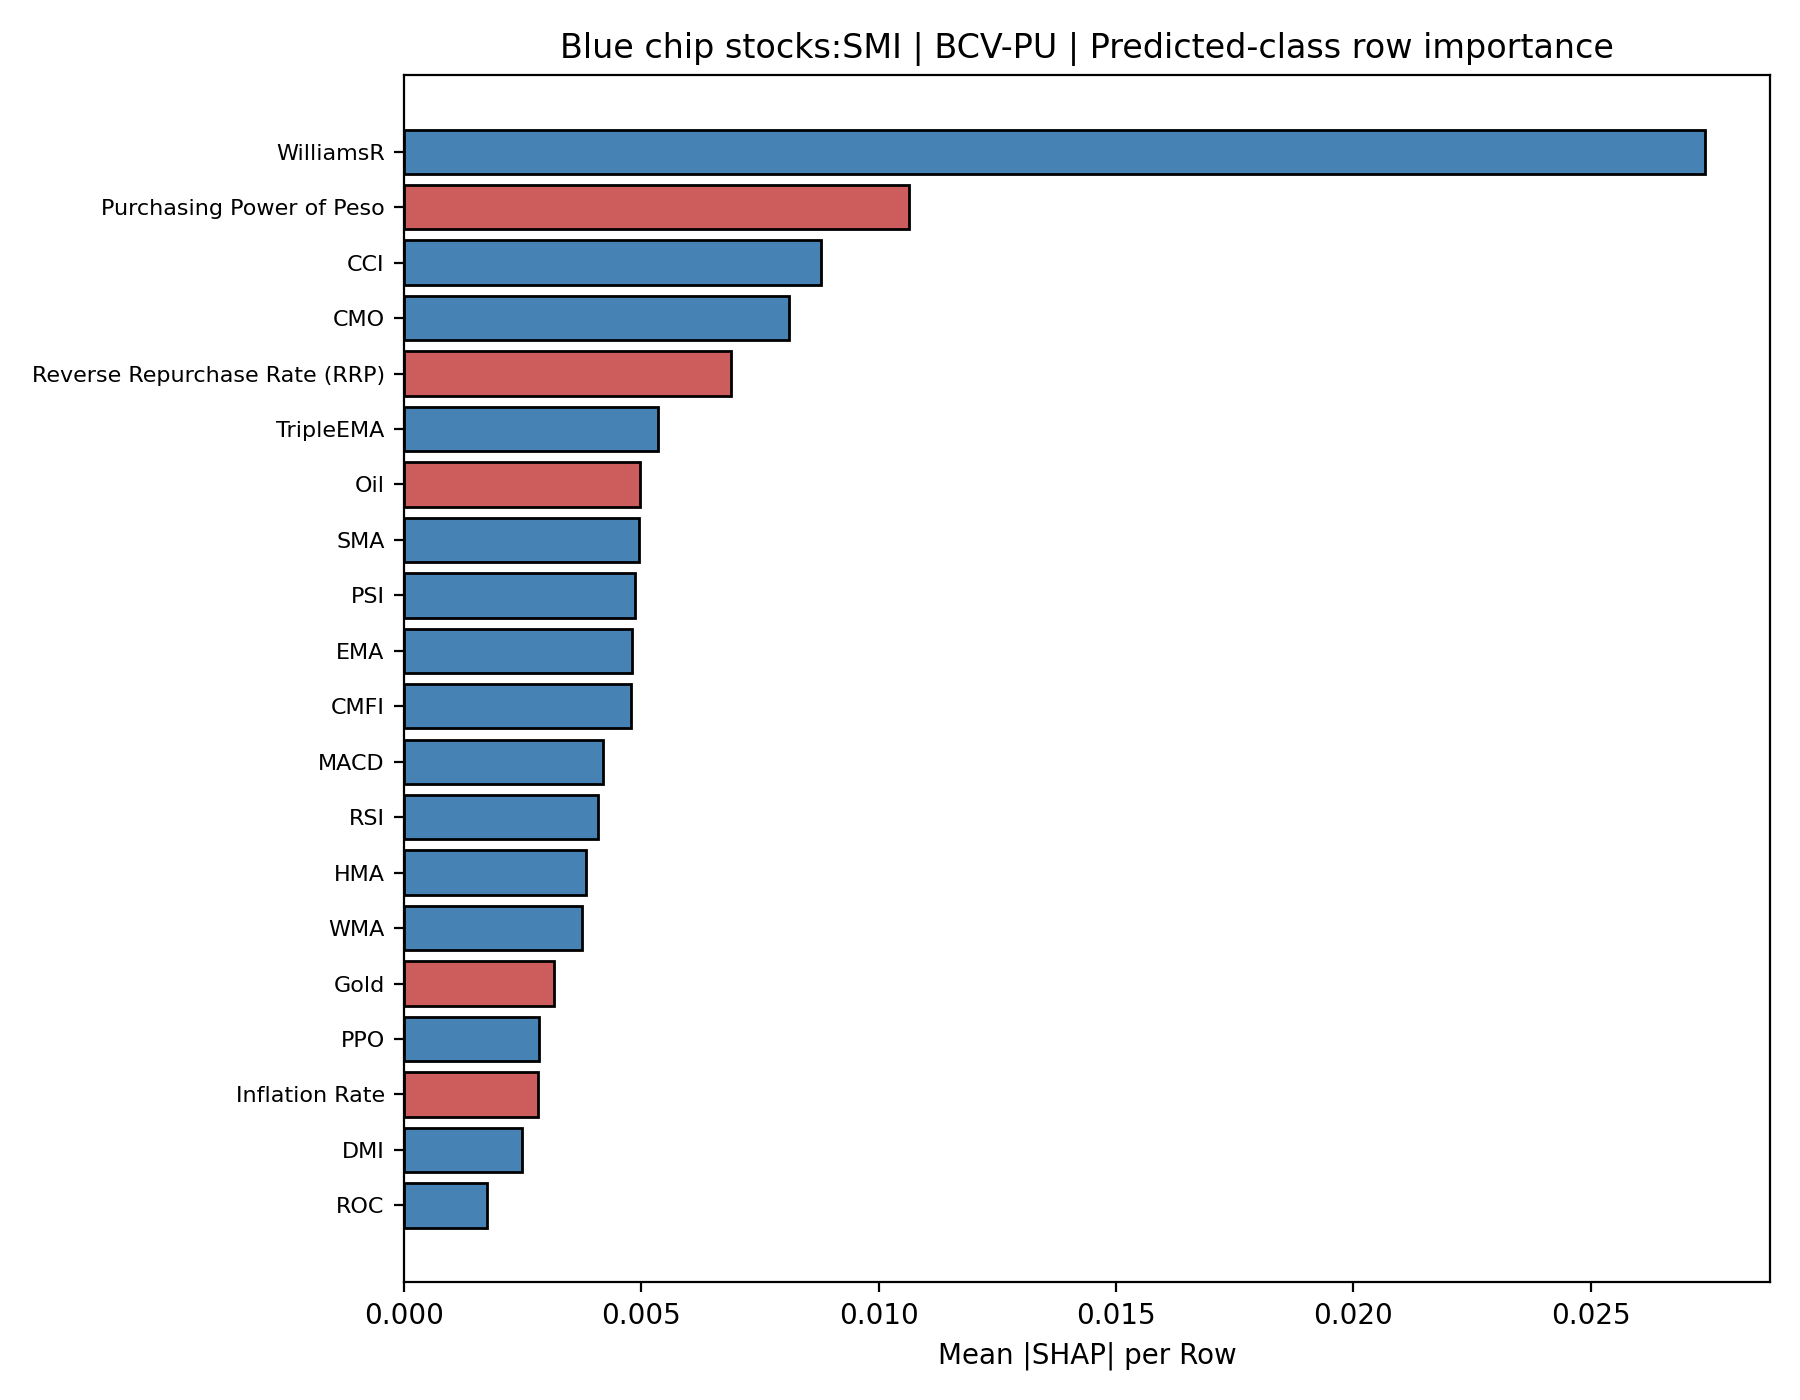
\includegraphics[width=0.32\textwidth]{../figures/SMI_PredictedClassRowImportance.png}
	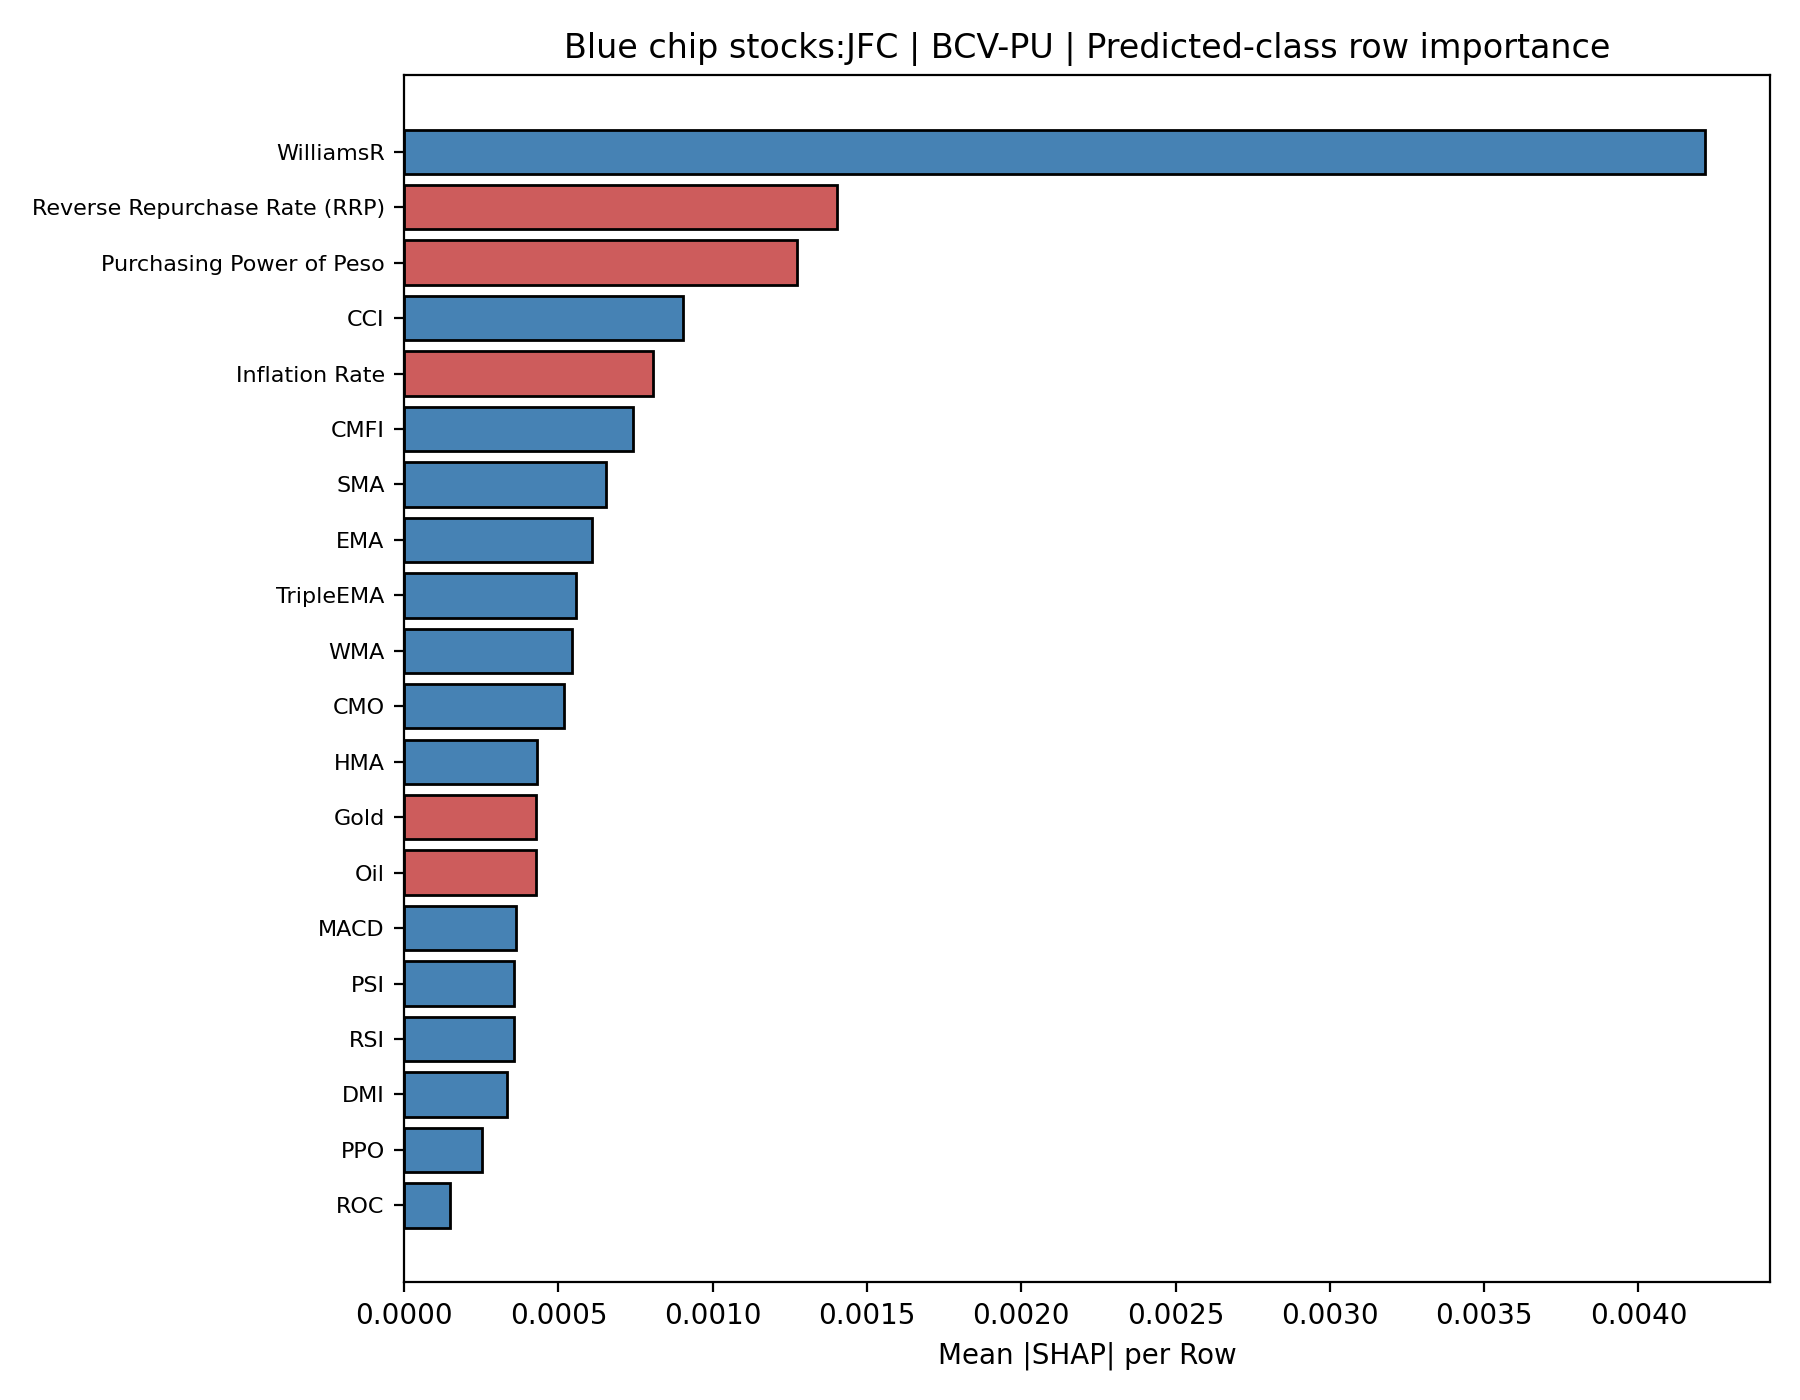
\includegraphics[width=0.32\textwidth]{../figures/JFC_PredictedClassRowImportance.png}
	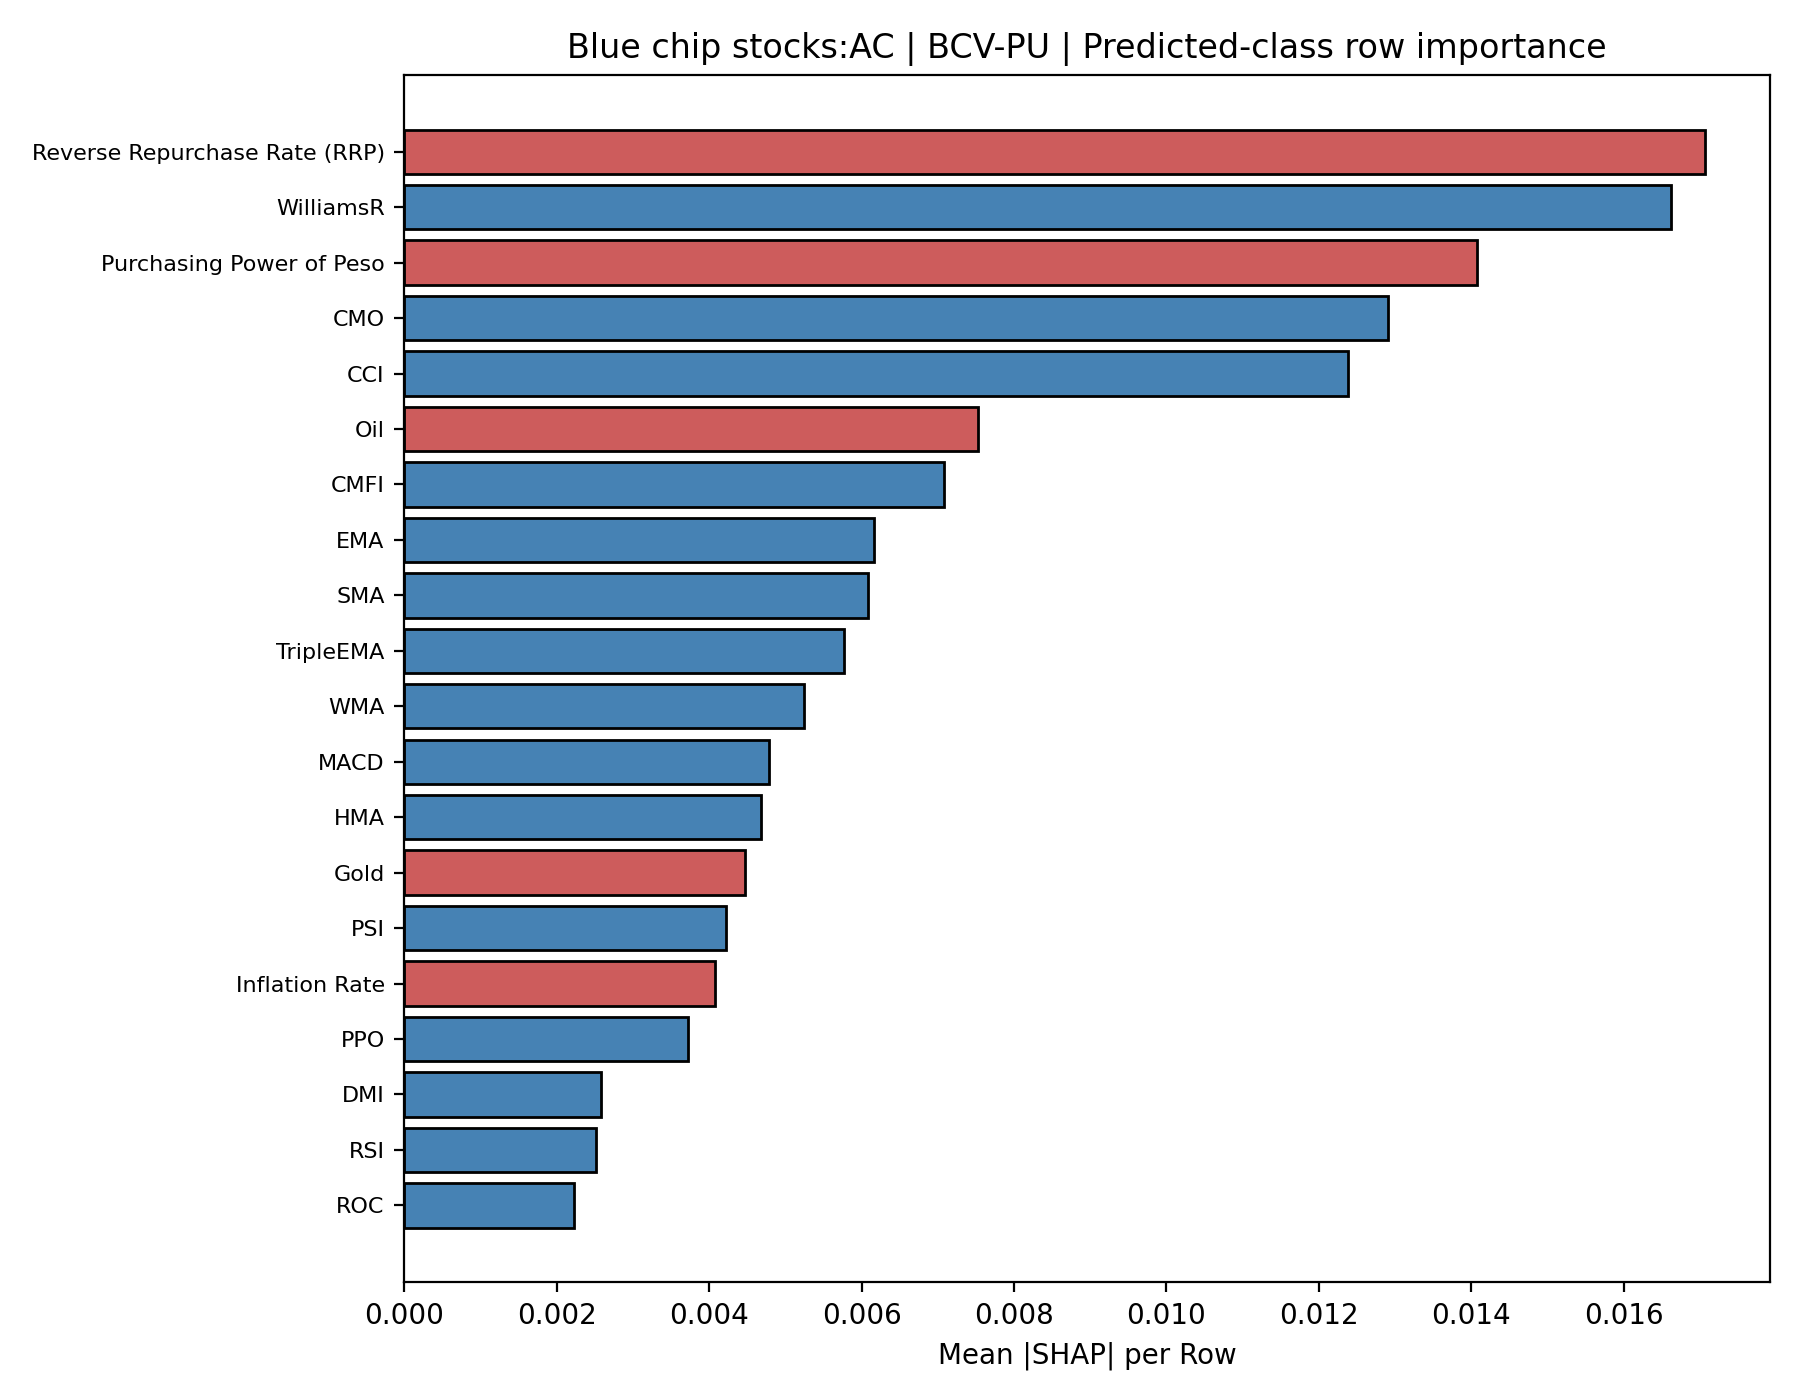
\includegraphics[width=0.32\textwidth]{../figures/AC_PredictedClassRowImportance.png}
	
	\captionof{figure}{Predicted-class SHAP row importance for selected blue-chip stocks under BCV-PU}
	\label{fig:app_shap_bluechip}
\end{center}

\begin{center}
	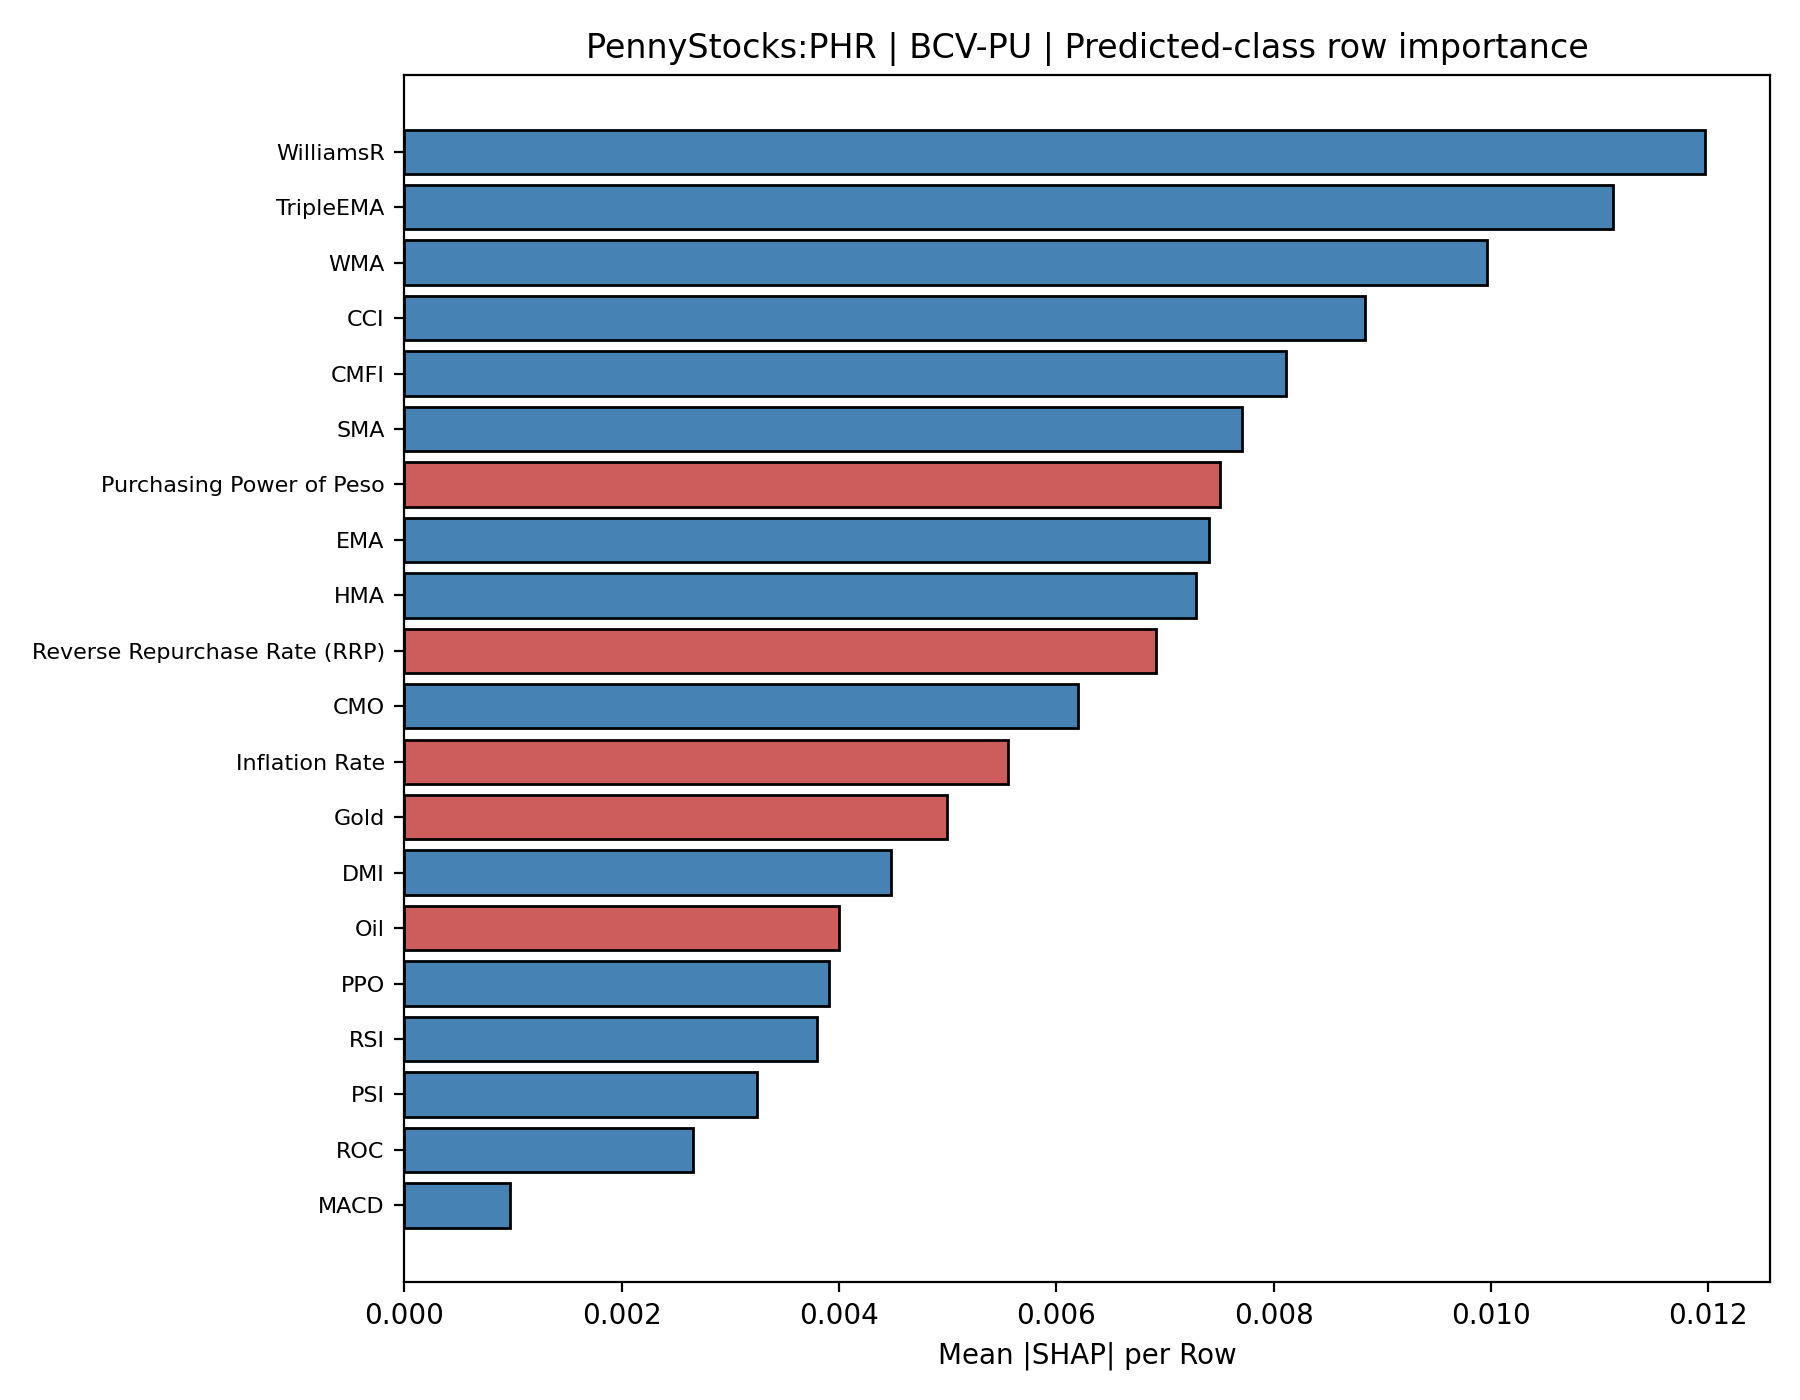
\includegraphics[width=0.32\textwidth]{../figures/PHR_PredictedClassRowImportance.png}
	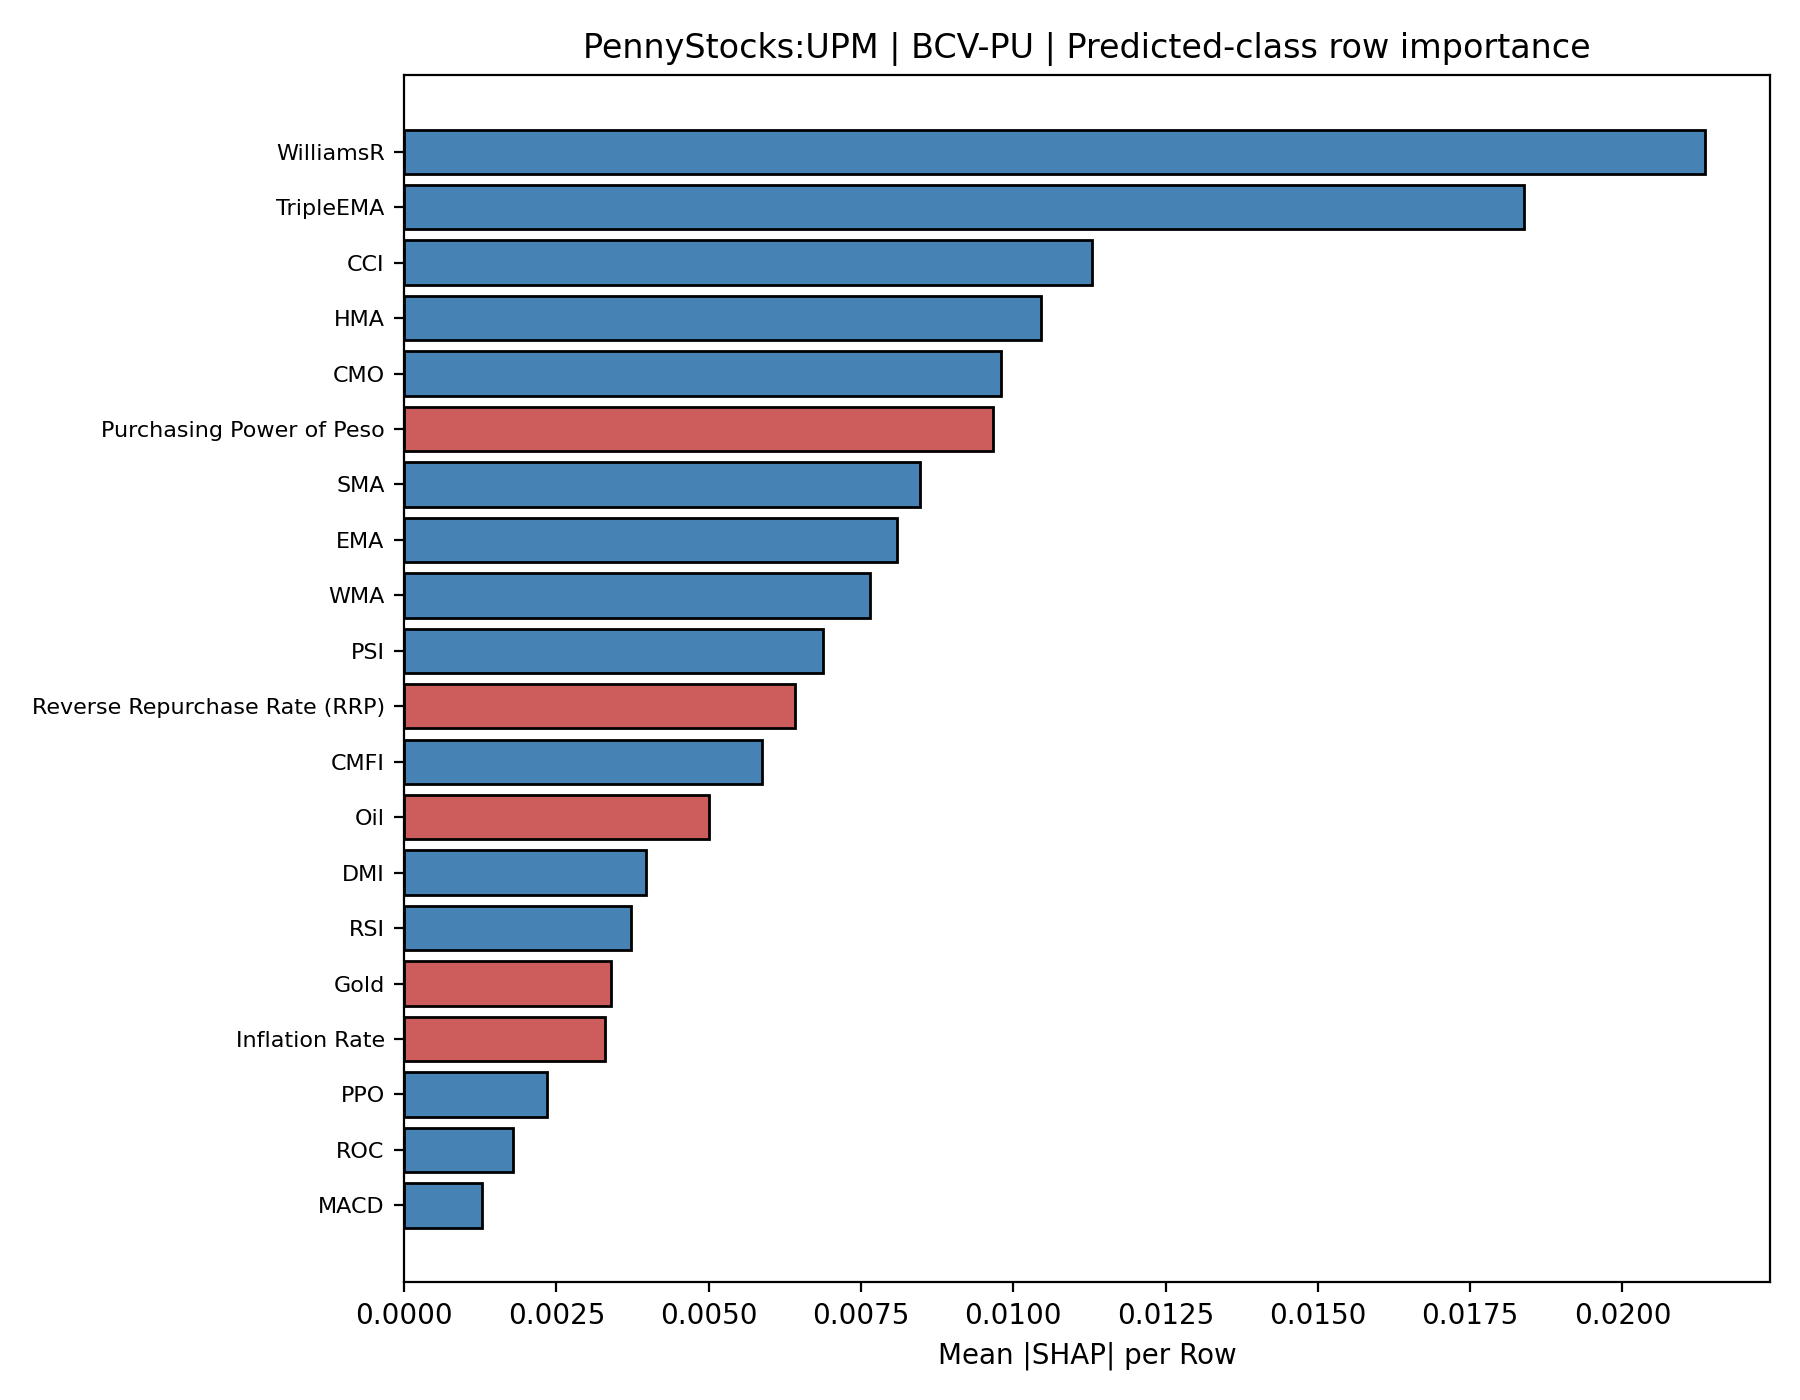
\includegraphics[width=0.32\textwidth]{../figures/UPM_PredictedClassRowImportance.png}
	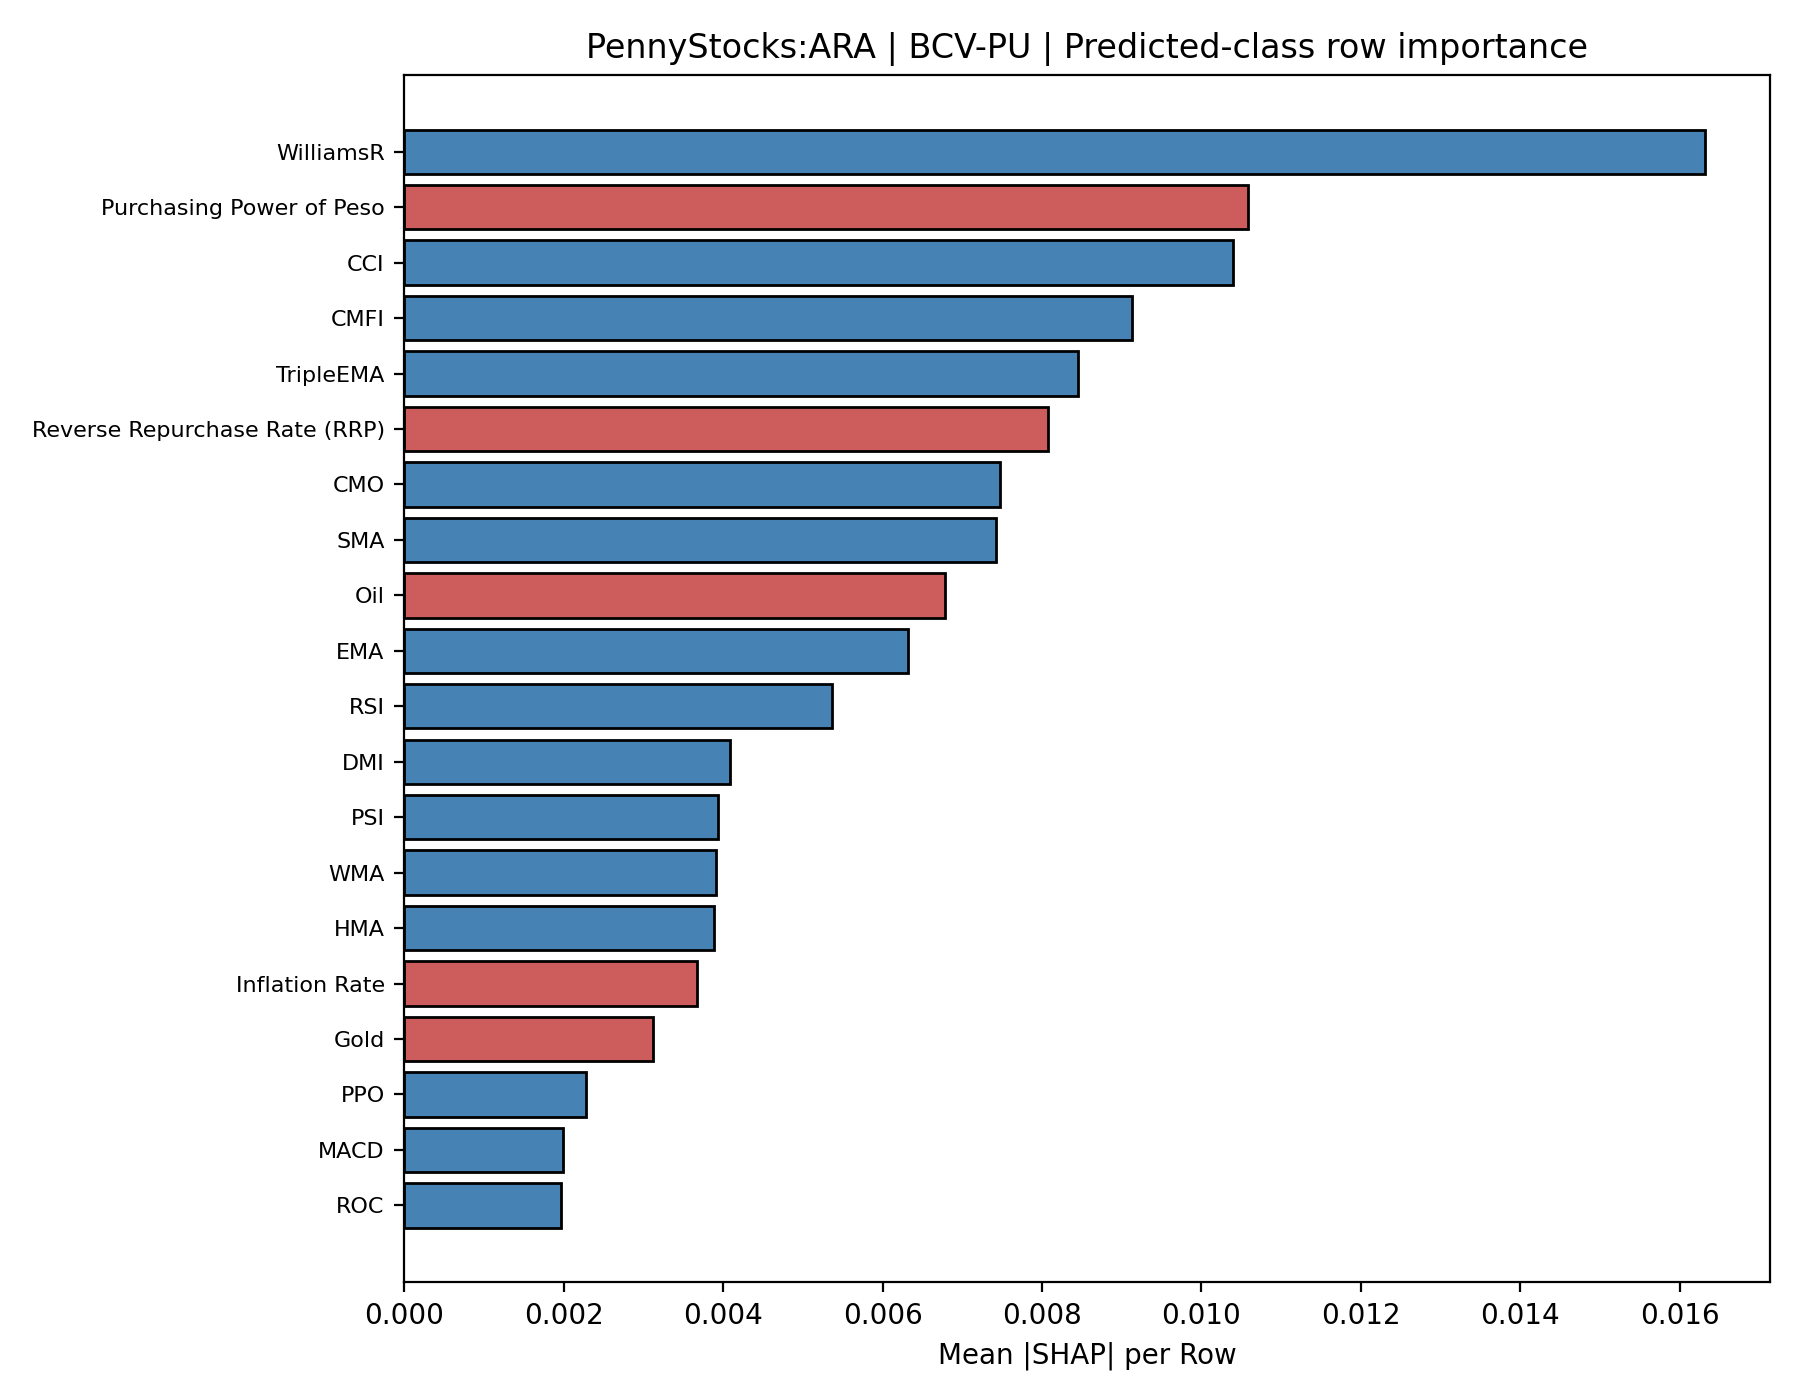
\includegraphics[width=0.32\textwidth]{../figures/ARA_PredictedClassRowImportance.png}
	
	\captionof{figure}{Predicted-class SHAP row importance for selected penny stocks under BCV-PU}
	\label{fig:app_shap_penny}
\end{center}

\begin{center}
	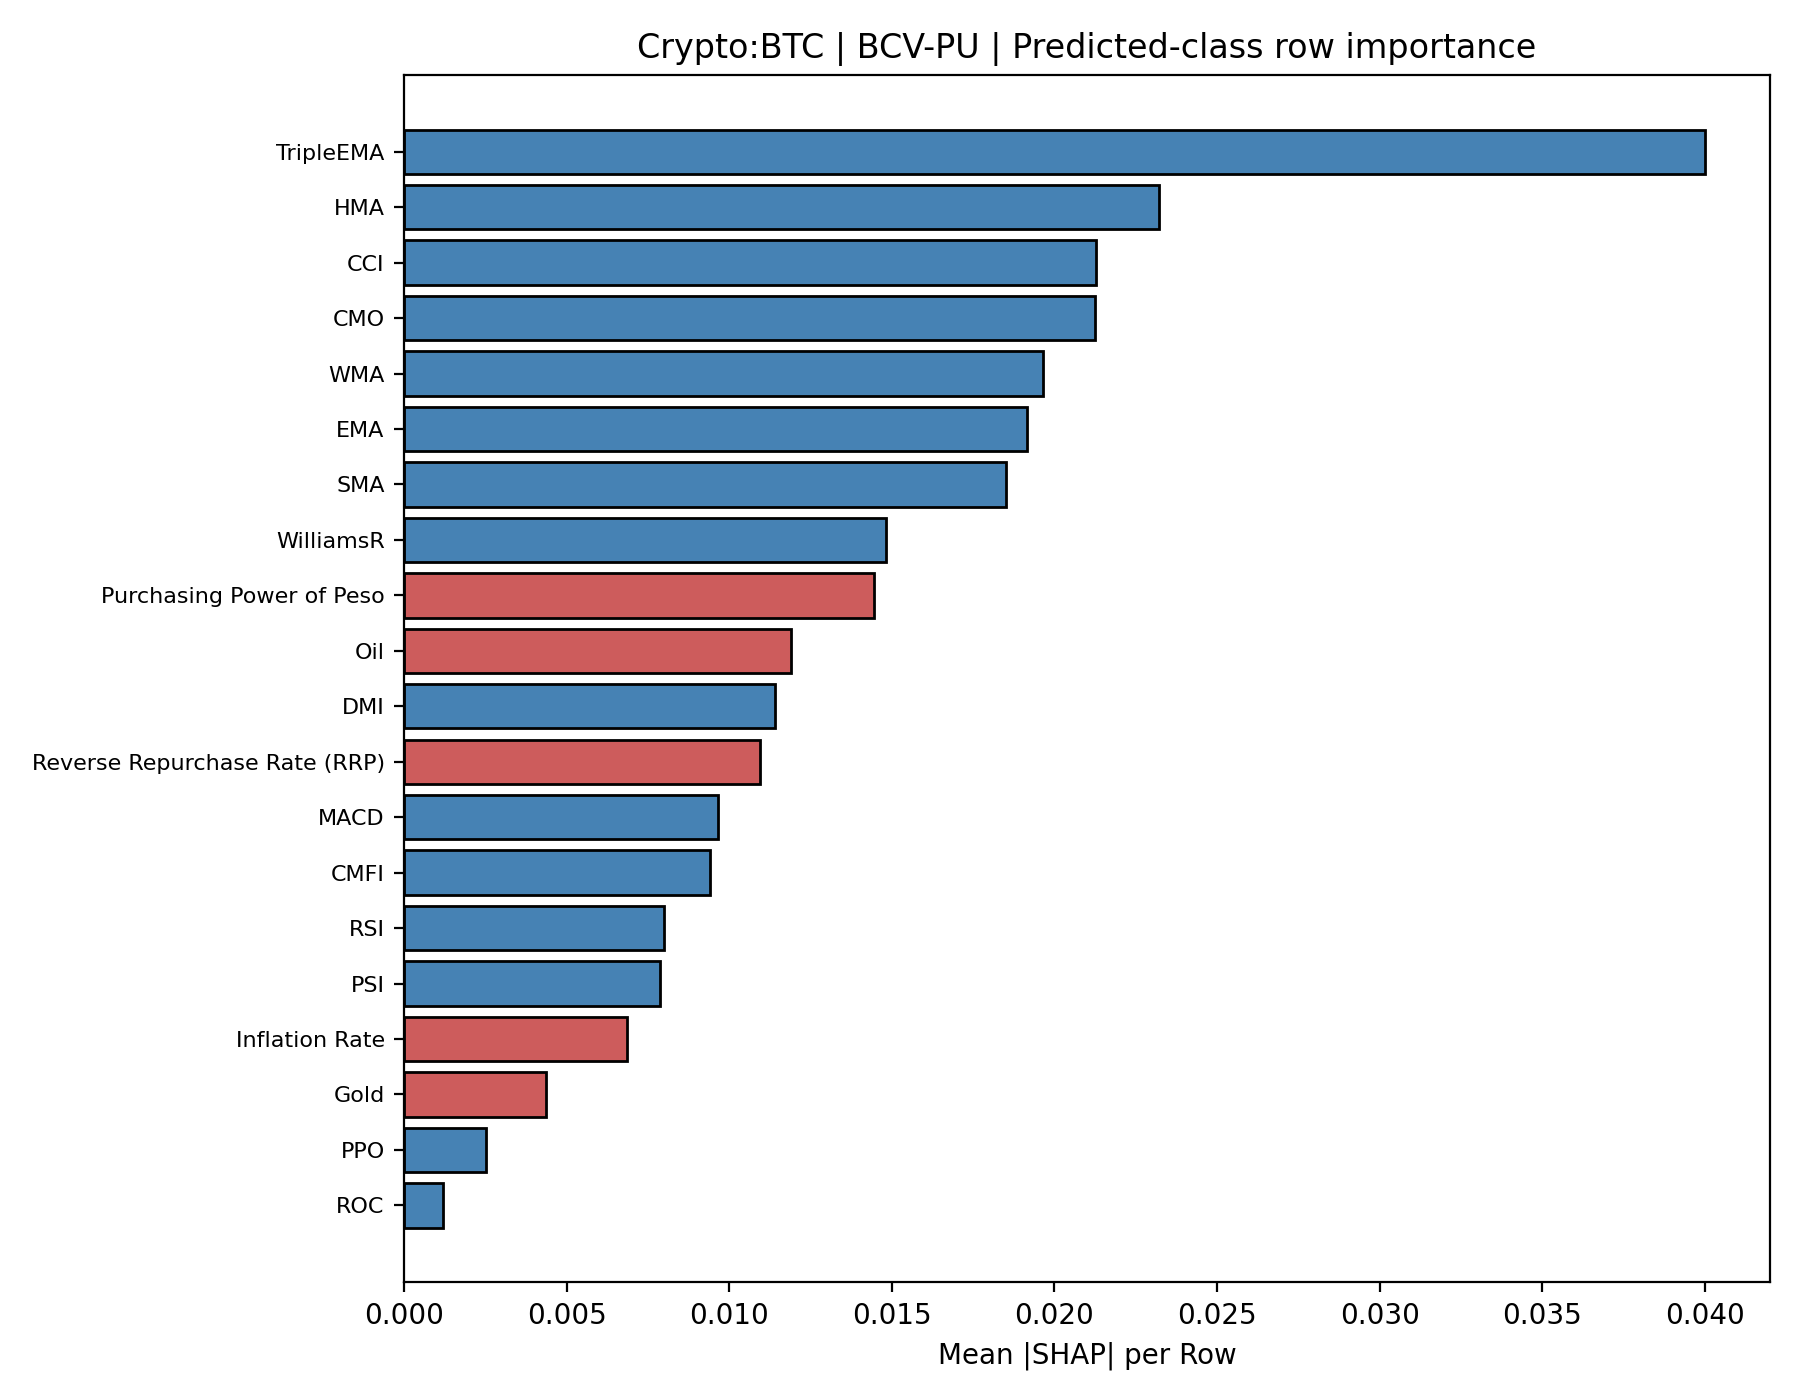
\includegraphics[width=0.32\textwidth]{../figures/BTC_PredictedClassRowImportance.png}
	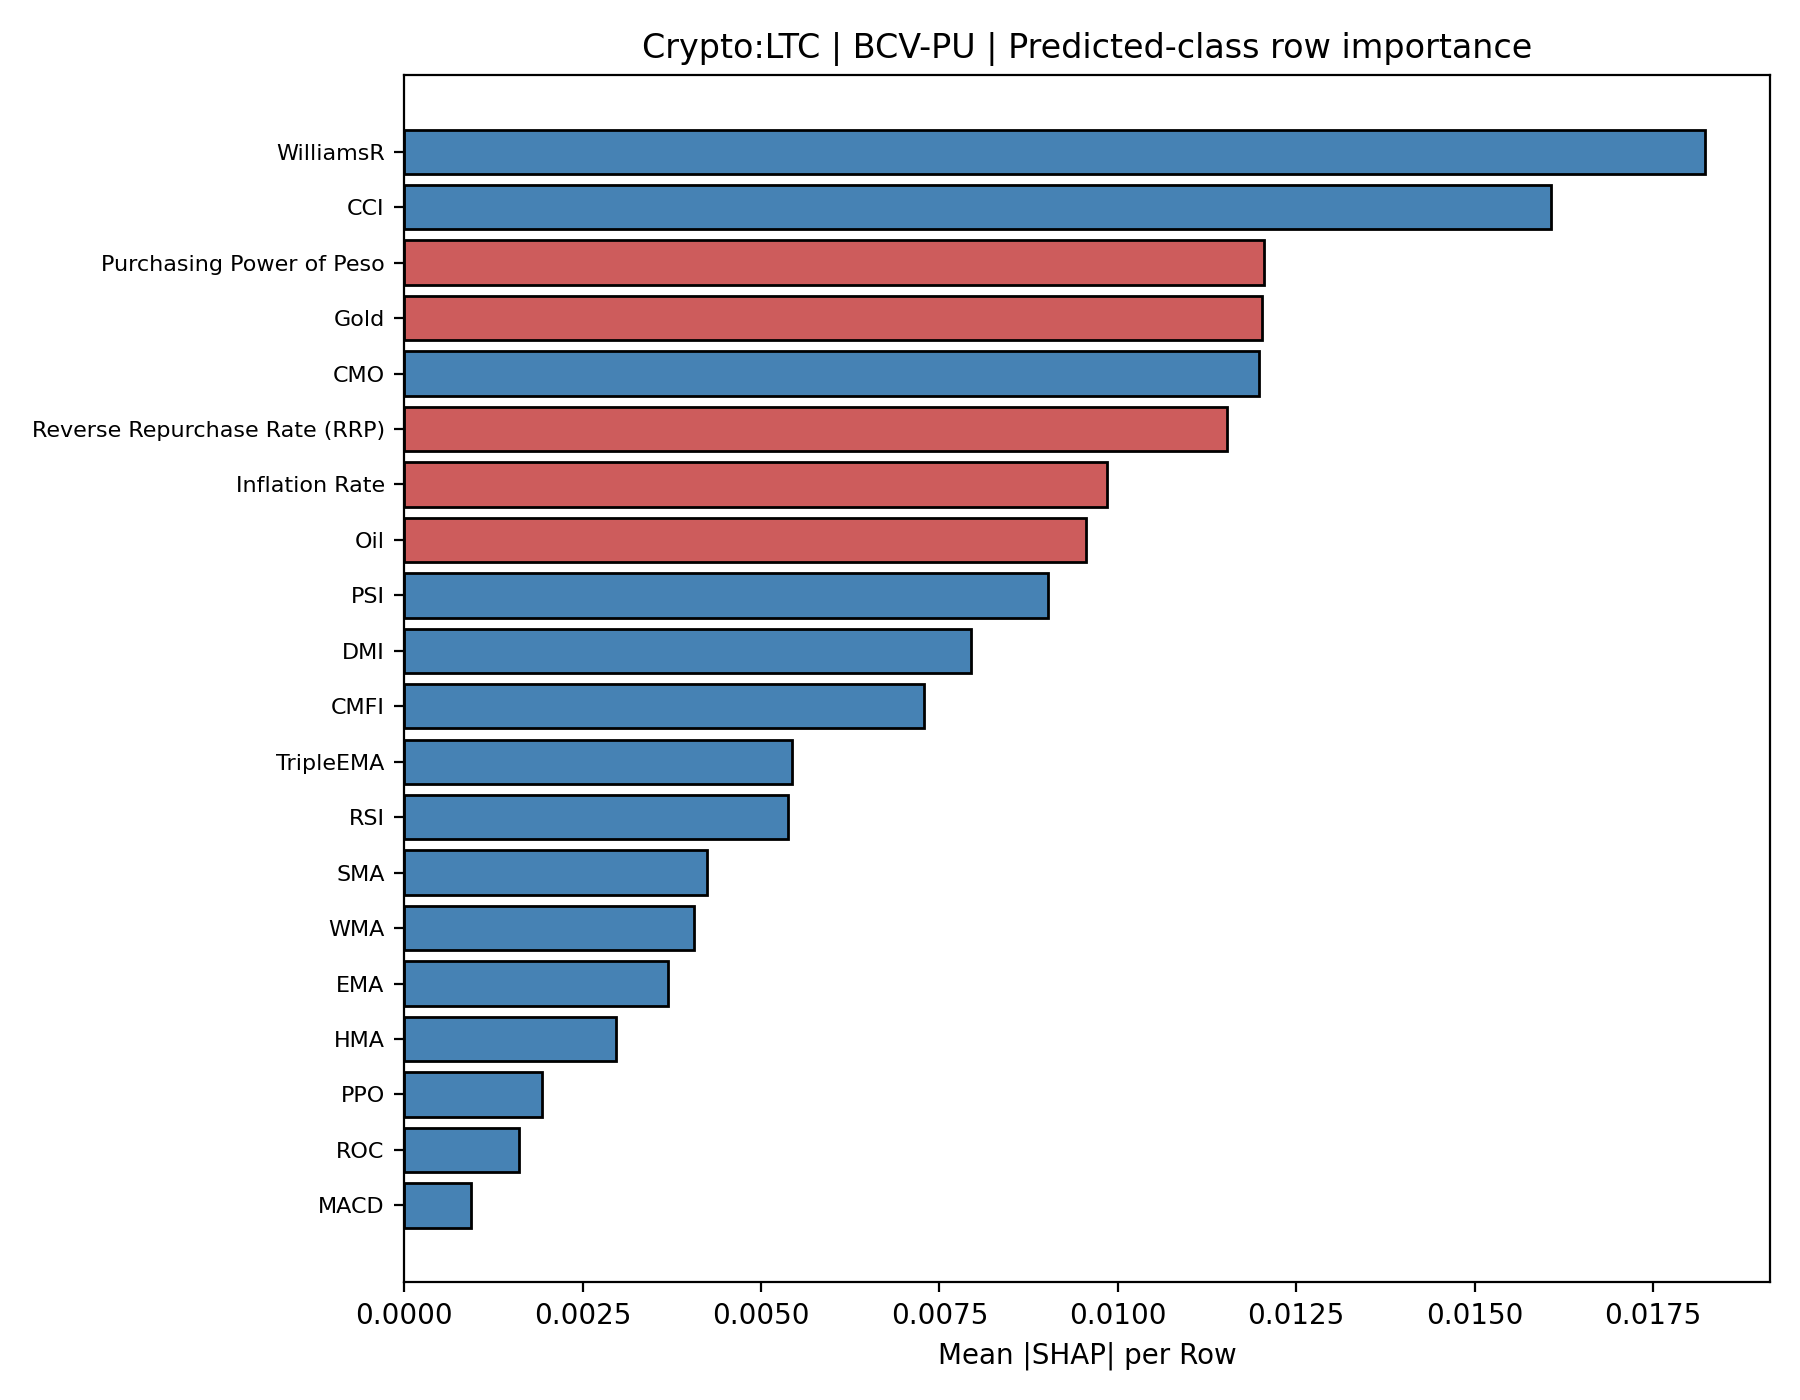
\includegraphics[width=0.32\textwidth]{../figures/LTC_PredictedClassRowImportance.png}
	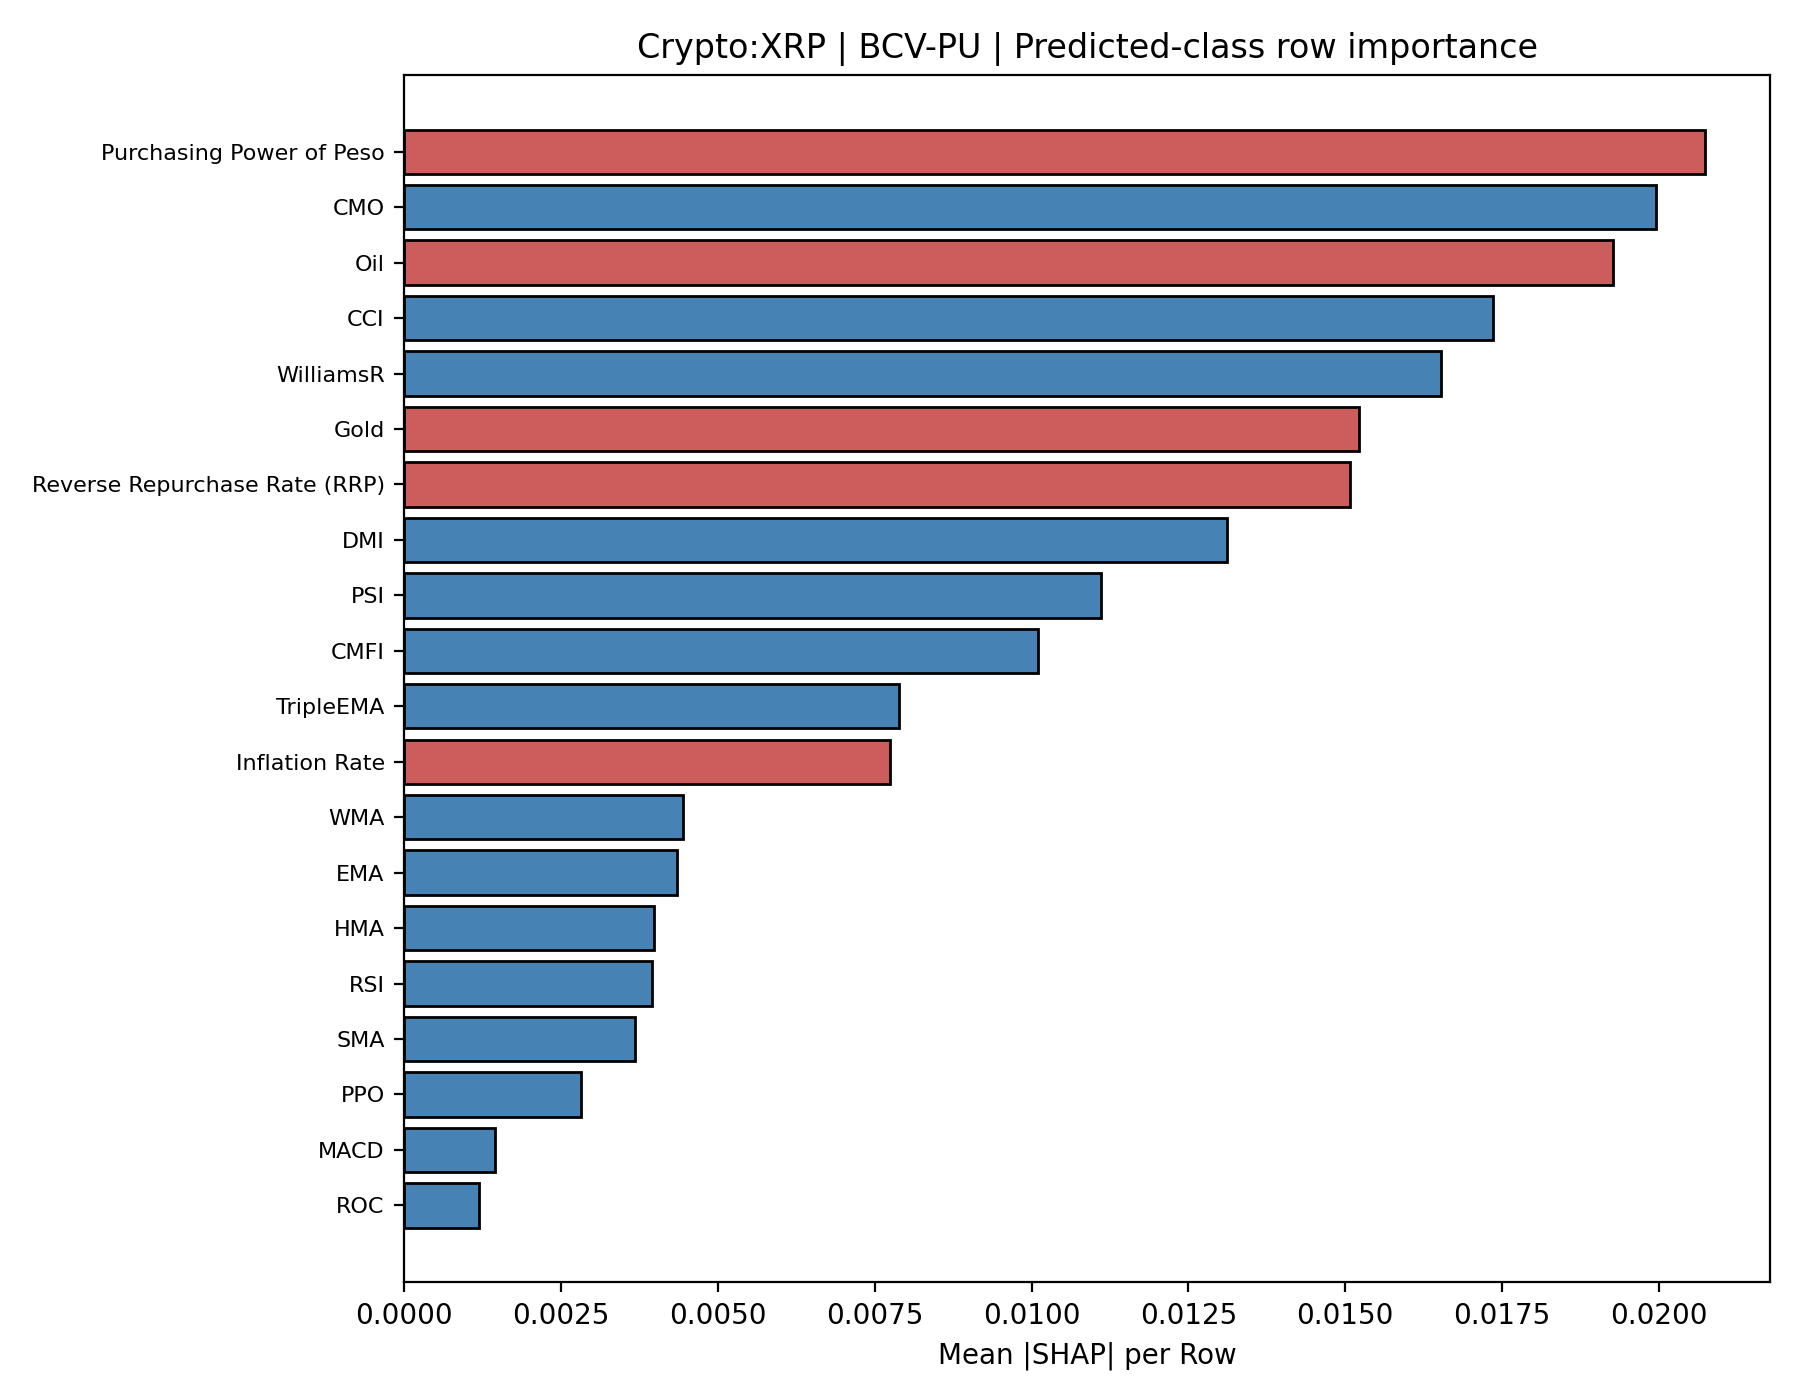
\includegraphics[width=0.32\textwidth]{../figures/XRP_PredictedClassRowImportance.png}
	
	\captionof{figure}{Predicted-class SHAP row importance for selected cryptocurrency assets under BCV-PU}
	\label{fig:app_shap_crypto}
\end{center}

\section{Confusion Matrices}
This section presents the confusion matrices for Blocked Cross-Validation with Partial Undersampling. 

\subsection{Ayala Corporation}

Table~\ref{tab:cm_ac} shows the CNN--TIC and CNN--MIC confusion matrix for Ayala Corporation under Blocked Cross-Validation with Partial Undersampling. Each row represents the true class, while each column represents the class predicted by the model.

\begin{center}
	\scriptsize
	\captionof{table}{Confusion matrix of Ayala Corporation in BCV-PU}
	\label{tab:cm_ac}
	\vspace{0.5em}
		{\renewcommand{\arraystretch}{1.2}
			\resizebox{\textwidth}{!}{%
			\begin{tabular}{llccc}
				\hline
				Model & True Class & Pred Sell & Pred Hold & Pred Buy \\
				\hline
				CNN--TIC & Sell & 26 & 21 & 0 \\
				& Hold & 75 & 361 & 112 \\
				& Buy & 0 & 12 & 37 \\
				\hline
				CNN--MIC & Sell & 30 & 17 & 0 \\
				& Hold & 83 & 377 & 88 \\
				& Buy & 0 & 14 & 35 \\
				\hline
			\end{tabular}
		}
	}
\end{center}

It can be seen that the number of correct CNN--MIC predicts the Hold class, while CNN--TIC does better in the Buy class. It is also noteworthy that there are more Hold to Buy misclassifications in CNN--TIC, which provides further explanation for the difference in their BCV-PU results.

\subsection{Jollibee Foods Corporation}
Table~\ref{tab:cm_jfc} shows the CNN--TIC and CNN--MIC confusion matrix for Jollibee Foods Corporation under Blocked Cross-Validation with Partial Undersampling. Each row represents the true class, while each column represents the class predicted by the model.

\begin{center}
	\centering
	\scriptsize
	\captionof{table}{Jollibee Foods Corporation's Confusion matrix in BCV-PU}
	\label{tab:cm_jfc}
	\renewcommand{\arraystretch}{1.2}
	\resizebox{\textwidth}{!}{%
		\begin{tabular}{llccc}
			\hline
			Model & True Class & Pred Sell & Pred Hold & Pred Buy \\
			\hline
			
			CNN--TIC & Sell & 25 & 23 & 0 \\
			& Hold & 69 & 390 & 93 \\
			& Buy & 0 & 6 & 37 \\
			\hline
			CNN--MIC & Sell & 30 & 18 & 0 \\
			& Hold & 85 & 418 & 49 \\
			& Buy & 0 & 23 & 20 \\
			\hline
		\end{tabular}%
	}
\end{center}

It can be seen that the number of correct CNN--MIC predicts the Hold class, while CNN--TIC performs better in the Buy class. It is also noteworthy that there are more Hold to Buy misclassifications in CNN--TIC, which provides further explanation for the difference in their BCV-PU results.
\subsection{SM Investments Corporation}

Table~\ref{tab:cm_smi} shows the CNN--TIC and CNN--MIC confusion matrix for SM Investments Corporation under Blocked Cross-Validation with Partial Undersampling. Each row represents the true class, while each column represents the class predicted by the model.

\begin{center}
	\centering
	\scriptsize
	\captionof{table}{Confusion matrix of SM Investments Corporation in BCV-PU}
	\label{tab:cm_smi}
	\renewcommand{\arraystretch}{1.2}
	\resizebox{\textwidth}{!}{%
		\begin{tabular}{llccc}
			\hline
			Model & True Class & Pred Sell & Pred Hold & Pred Buy \\
			\hline
			
			CNN--TIC & Sell & 12 & 28 & 0 \\
			& Hold & 17 & 504 & 40 \\
			& Buy & 0 & 21 & 21 \\
			\hline
			CNN--MIC & Sell & 22 & 18 & 0 \\
			& Hold & 50 & 459 & 52 \\
			& Buy & 0 & 15 & 27 \\
			\hline
		\end{tabular}%
	}
\end{center}
It can be seen that CNN--TIC has a higher number of correct predictions in the Hold class, and CNN--MIC has a clearer advantage in the Buy class. It is also noteworthy that CNN--MIC has a higher number of misclassifications from Hold to Buy, which provides further explanation for the difference in their BCV-PU results.



\subsection{Araneta Properties}

The confusion matrix of CNN--TIC and CNN--MIC for Araneta Properties under Blocked Cross-Validation with Partial Undersampling is shown in Table~\ref{tab:cm_ara}. Each row represents the true class, while each column represents the class predicted by the model.

\begin{center}
	\centering
	\scriptsize
	\captionof{table}{Confusion matrix of Araneta Properties in BCV-PU}
	\label{tab:cm_ara}
	\renewcommand{\arraystretch}{1.2}
	\resizebox{\textwidth}{!}{%
		\begin{tabular}{llccc}
			\hline
			Model & True Class & Pred Sell & Pred Hold & Pred Buy \\
			\hline
			
			CNN--TIC & Sell & 18 & 24 & 1 \\
			& Hold & 42 & 260 & 239 \\
			& Buy & 0 & 6 & 40 \\
			\hline
			CNN--MIC & Sell & 11 & 30 & 2 \\
			& Hold & 20 & 230 & 291 \\
			& Buy & 0 & 3 & 43 \\
			\hline
		\end{tabular}%
	}
\end{center}

It can be seen that the number of correct predictions is higher CNN--TIC in the Hold class, and CNN--MIC also has a clearer advantage in the Buy class. It is also noteworthy that there are more misclassifications from Hold to Buy in CNN--MIC, which provides further explanation for the difference in their BCV-PU results.

\subsection{PH Resorts Group}

The confusion matrix of CNN--TIC and CNN--MIC for PH Resorts Group under Blocked Cross-Validation with Partial Undersampling can be seen in Table~\ref{tab:cm_phr}. Each row refers to the true class, while each column refers to the class predicted by the model.

\begin{center}
	\centering
	\scriptsize
	\captionof{table}{Confusion matrix of PH Resorts Group in BCV-PU}
	\label{tab:cm_phr}
	\renewcommand{\arraystretch}{1.2}
	\resizebox{\textwidth}{!}{%
		\begin{tabular}{llccc}
			\hline
			Model & True Class & Pred Sell & Pred Hold & Pred Buy \\
			\hline
			
			CNN--TIC & Sell & 0 & 42 & 0 \\
			& Hold & 0 & 467 & 77 \\
			& Buy & 0 & 40 & 17 \\
			\hline
			CNN--MIC & Sell & 2 & 34 & 6 \\
			& Hold & 3 & 205 & 336 \\
			& Buy & 0 & 1 & 56 \\
			\hline
		\end{tabular}%
	}
\end{center}

It can be seen that the number of correct predictions is higher for CNN--TIC in the Hold class, and CNN--MIC also has a clearer advantage in the Buy class. It is also noteworthy that there are more misclassifications from Hold to Buy in CNN--MIC, which provides further explanation for the difference in their BCV-PU results.\subsection{United Paragon Mining Corporation}

Table~\ref{tab:cm_upm} shows the CNN--TIC and CNN--MIC confusion matrix for United Paragon Mining Corporation under Blocked Cross-Validation with Partial Undersampling. Each row represents the true class, while each column represents the class predicted by the model.

\begin{center}
	\centering
	\scriptsize
	\captionof{table}{Confusion matrix of United Paragon Mining Corporation in BCV-PU}
	\label{tab:cm_upm}
	\renewcommand{\arraystretch}{1.2}
	\resizebox{\textwidth}{!}{%
		\begin{tabular}{llccc}
			\hline
			Model & True Class & Pred Sell & Pred Hold & Pred Buy \\
			\hline
			
			CNN--TIC & Sell & 22 & 4 & 0 \\
			& Hold & 53 & 174 & 22 \\
			& Buy & 0 & 15 & 15 \\
			\hline
			CNN--MIC & Sell & 22 & 4 & 0 \\
			& Hold & 51 & 123 & 75 \\
			& Buy & 0 & 2 & 28 \\
			\hline
		\end{tabular}%
	}
\end{center}

It can be seen that the number of correct predictions is higher CNN--TIC in the Hold class, and CNN--MIC also has a clearer advantage in the Buy class. It is also noteworthy that there are more misclassifications from Hold to Buy in CNN--MIC, which provides further explanation for the difference in their BCV-PU results.

\subsection{Bitcoin}

The confusion matrix of CNN--TIC and CNN--MIC for Bitcoin under Blocked Cross-Validation with Partial Undersampling is shown in Table~\ref{tab:cm_btc}. Each row refers to the true class, while each column refers to the class predicted by the model.

\begin{center}
	\centering
	\scriptsize
	\captionof{table}{Confusion matrix of Bitcoin in BCV-PU}
	\label{tab:cm_btc}
	\renewcommand{\arraystretch}{1.2}
	\resizebox{\textwidth}{!}{%
		\begin{tabular}{llccc}
			\hline
			Model & True Class & Pred Sell & Pred Hold & Pred Buy \\
			\hline
			
			CNN--TIC & Sell & 26 & 38 & 0 \\
			& Hold & 125 & 702 & 12 \\
			& Buy & 11 & 45 & 3 \\
			\hline
			CNN--MIC & Sell & 33 & 31 & 0 \\
			& Hold & 195 & 640 & 4 \\
			& Buy & 23 & 30 & 6 \\
			\hline
		\end{tabular}%
	}
\end{center}

It can be seen that the number of correct predictions is higher CNN--TIC in the Hold class, and CNN--MIC also has a clearer advantage in the Buy class. It is also noteworthy that there are more misclassifications from Hold to Buy in CNN--TIC, which provides further explanation for the difference in their BCV-PU results.

\subsection{Litecoin}

The confusion matrix of CNN--TIC and CNN--MIC for Litecoin under Blocked Cross-Validation with Partial Undersampling is shown in Table~\ref{tab:cm_ltc}. Each row refers to the true class, while each column refers to the class predicted by the model.

\begin{center}
	\centering
	\scriptsize
	\captionof{table}{Confusion matrix of Litecoin in BCV-PU}
	\label{tab:cm_ltc}
	\renewcommand{\arraystretch}{1.2}
	\resizebox{\textwidth}{!}{%
		\begin{tabular}{llccc}
			\hline
			Model & True Class & Pred Sell & Pred Hold & Pred Buy \\
			\hline
			
			CNN--TIC & Sell & 29 & 37 & 0 \\
			& Hold & 58 & 652 & 125 \\
			& Buy & 0 & 12 & 49 \\
			\hline
			CNN--MIC & Sell & 20 & 46 & 0 \\
			& Hold & 45 & 694 & 96 \\
			& Buy & 0 & 17 & 44 \\
			\hline
		\end{tabular}%
	}
\end{center}
It can be seen that CNN--MIC has a higher number of correct predictions for the Hold class, while CNN--TIC has a better performance for the Buy class. It is also noteworthy that CNN--TIC has a higher number of misclassifications from Hold to Buy, which further explains the difference in their BCV-PU results.

\subsection{XRP}

The confusion matrix of CNN--TIC and CNN--MIC for XRP under Blocked Cross-Validation with Partial Undersampling is shown in Table~\ref{tab:cm_xrp}. Each row represents the true class, while each column represents the class predicted by the model.

\begin{center}
	\centering
	\scriptsize
	\captionof{table}{XRP Confusion matrix in BCV-PU}
	\label{tab:cm_xrp}
	\renewcommand{\arraystretch}{1.2}
	\resizebox{\textwidth}{!}{%
		\begin{tabular}{llccc}
			\hline
			Model & True Class & Pred Sell & Pred Hold & Pred Buy \\
			\hline
			
			CNN--TIC & Sell & 59 & 5 & 0 \\
			& Hold & 289 & 477 & 72 \\
			& Buy & 11 & 21 & 27 \\
			\hline
			CNN--MIC & Sell & 56 & 8 & 0 \\
			& Hold & 330 & 486 & 22 \\
			& Buy & 14 & 39 & 6 \\
			\hline
		\end{tabular}%
	}
\end{center}

It can be seen that the number of correct predictions is higher CNN--MIC performs better in the Hold class, while CNN--TIC performs better in the Buy class. It is also noteworthy that there are more misclassifications from Hold to Buy in CNN--TIC, which further explains the difference in their BCV-PU results.

% ------------------------------------------------------------------------

\setlinespacing{1.44}
%\bibliographystyle{amsplain}
\newpage
\printbibliography
\end{document}
% ------------------------------------------------------------------------